%
% This file is released under the Creative Commons CC-BY-SA
% 4.0 License; see: 
%
% https://creativecommons.org/licenses/by-sa/4.0/
%
% AUTHORS
%	Jérôme KUNEGIS <jerome.kunegis@unamur.be> 
%	Daniel DÜNKER <dduenker@uni-koblenz.de>
%

\documentclass{article}

\usepackage{hyperref}
\pdfoutput=1

\usepackage[utf8]{inputenc}
\usepackage{amsmath}
\usepackage{amssymb}
\usepackage{booktabs}
\usepackage{graphicx}
\usepackage{grffile}
\usepackage{subfigure}
\usepackage{marvosym} % for \Clocklogo
\usepackage{color}
\usepackage{marginnote}
\usepackage{textcomp} % for \textlangle, \textrangle 
\usepackage{array}
\usepackage{wasysym} % for \newmoon
\usepackage{tikz}
\usepackage{natbib}
\usepackage[nottoc]{tocbibind}
\usepackage{wrapfig}
\usepackage{longtable}

\newcommand{\wPlot}{0.45\textwidth}
\newcommand{\wFull}{0.95\textwidth}
\newcommand{\wOnePointFive}{0.8\textwidth}
\newcommand{\wTwo}{0.45\textwidth}
\newcommand{\wThree}{0.31\textwidth}
\newcommand{\wFour}{0.24\textwidth}

%auto-ignore
% Auto-generated by Stu on jeudi 19 octobre 2017, 11:19:34 (UTC+0200)
\definecolor{colorAffiliation}{rgb}{1, 0.4, 0.4}
\definecolor{colorAnimal}{rgb}{0.24, 0.84, 0.32}
\definecolor{colorAuthorship}{rgb}{0.8, 0, 1}
\definecolor{colorCitation}{rgb}{0.10, 0.16, 0.50}
\definecolor{colorCoauthorship}{rgb}{0.81, 0.90, 0.12}
\definecolor{colorCocitation}{rgb}{0.79, 0.58, 0.15}
\definecolor{colorCommunication}{rgb}{0, 0, 1}
\definecolor{colorComputer}{rgb}{0.56, 0.32, 0.69}
\definecolor{colorFeature}{rgb}{0.55, 0.55, 1}
\definecolor{colorFolksonomy}{rgb}{0.08, 0.83, 0.23}
\definecolor{colorHumanContact}{rgb}{0.86, 0.81, 0.59}
\definecolor{colorHumanSocial}{rgb}{0.42, 0.42, 0.37}
\definecolor{colorHyperlink}{rgb}{1, 0.62, 0}
\definecolor{colorInfrastructure}{rgb}{1.0, 0.2, 0.2}
\definecolor{colorInteraction}{rgb}{0.25, 0.75, 0.25}
\definecolor{colorLexical}{rgb}{0, 1, 0}
\definecolor{colorMetabolic}{rgb}{0.58, 0.70, 0.67}
\definecolor{colorMisc}{rgb}{0.85, 0.95, 0.59}
\definecolor{colorOnlineContact}{rgb}{0.27, 0.54, 0.95}
\definecolor{colorRating}{rgb}{0.70, 0.70, 0}
\definecolor{colorSocial}{rgb}{0.10, 0.10, 0.38}
\definecolor{colorSoftware}{rgb}{0.10, 0.37, 0.10}
\definecolor{colorText}{rgb}{0.43, 0.52, 0.82}
\definecolor{colorTrophic}{rgb}{0.40, 0.42, 0.61}


\begin{document}

\title{
  
\includegraphics[width=3cm]{konect-logo} \\
  \vspace{1cm}
         {\Huge Handbook of Network Analysis} \\
         KONECT project
}

\author{
  Jérôme Kunegis \\
  University of Namur, Belgium \\
  naXys -- Namur Center for Complex Systems \\
  {\small with web hosting provided by the Institute of Web Science and
    Technologies (WeST)} \\ 
  {\small at the University of Koblenz--Landau, Germany} \\
  {\small \href{http://konect.uni-koblenz.de/}{konect.uni-koblenz.de}}
}

\maketitle

\section*{Abstract}
This is the handbook for the KONECT project, a scientific project to
archive network datasets, compute systematic network theoretic
statistics about them, visualize their properties, and provide
corresponding data and Free Software tools to researchers in all related
fields of research related to network analysis and graph mining, by
Jérôme Kunegis at the Namur Center for Complex Systems (naXys) at the
University of Namur, Belgium.  The name \emph{KONECT} stands for
\emph{Koblenz Network Collection}, as large parts of the KONECT project
were initially initiated as part of the PhD thesis of Jérôme Kunegis at
the University of Koblenz--Landau in Germany in 2011.  This handbook
documents all methods, definitions and conventions used in the project,
and serves as a general handbook of network mining, with an emphasis on
spectral graph theoretical methods, i.e., such methods that are based on
the use of specific characteristic matrices of graphs. 

\thispagestyle{empty}
\newpage

\section{Introduction}
Everything is a network~-- whenever we look at the interactions between
things, a network is formed implicitly.  In the areas of data mining,
machine learning, information retrieval, etc., networks are modeled
as \emph{graphs}.  Many, if not most problem types can be applied to
graphs: clustering, classification, prediction, pattern recognition, and
others.  Networks arise in almost all areas of research, commerce and
daily life in the form of social networks, road networks, communication
networks, trust networks, hyperlink networks, chemical interaction
networks, neural networks, collaboration networks and lexical networks.
The content of text documents is routinely modeled as document--word
networks, taste as person--item networks and trust as person--person
networks.  In recent years, whole database systems have appeared
specializing in storing networks.  In fact, a majority of research
projects in the areas of web mining, web science and related areas uses
datasets that can be understood as networks.  Unfortunately, results
from the literature can often not be compared easily because
they use different datasets. What is more, different network datasets
have slightly different properties, such as allowing multiple or only
single edges between two nodes.  In order to provide a unified view on
such network datasets, and to allow the application of network analysis
methods across disciplines, the KONECT project defines a comprehensive
network taxonomy and provides a consistent access to network datasets.
To validate this approach on real-world data from the Web, KONECT
also provides a large number (210+) of network datasets of different
types and different application areas. 

KONECT, the \underline{Ko}blenz \underline{Ne}twork \underline
Collec\underline tion, contains 214 network datasets as of October 2014.
In addition to these datasets, KONECT consists of Matlab code to
generate statistics and plots about them, which are shown on the
KONECT
website\footnote{\href{http://konect.uni-koblenz.de/}{konect.uni-koblenz.de}}.
KONECT contains networks of all sizes, from small classical datasets
from the social sciences such as Kenneth Read's Highland Tribes network
with 16 vertices and 58 edges
(\href{http://konect.uni-koblenz.de/networks/ucidata-gama}{\textsf{HT}}),
to the Twitter social network with 52 million nodes and 1.9 billion
edges
(\href{http://konect.uni-koblenz.de/networks/twitter_mpi}{\textsf{TF}}).
Figure~\ref{fig:scatter.size.avgdegree} shows a scatter plot of all
networks by the number of nodes and the average degree in the network.
Each network in KONECT is represented by a unique two- or
three-character code which we write in a \textsf{sans-serif font}, and
is indicated in parentheses as used previously in this paragraph. The
full list of codes is given
online.\footnote{\href{http://konect.uni-koblenz.de/networks}{konect.uni-koblenz.de/networks}}

\begin{figure}
  \centering
  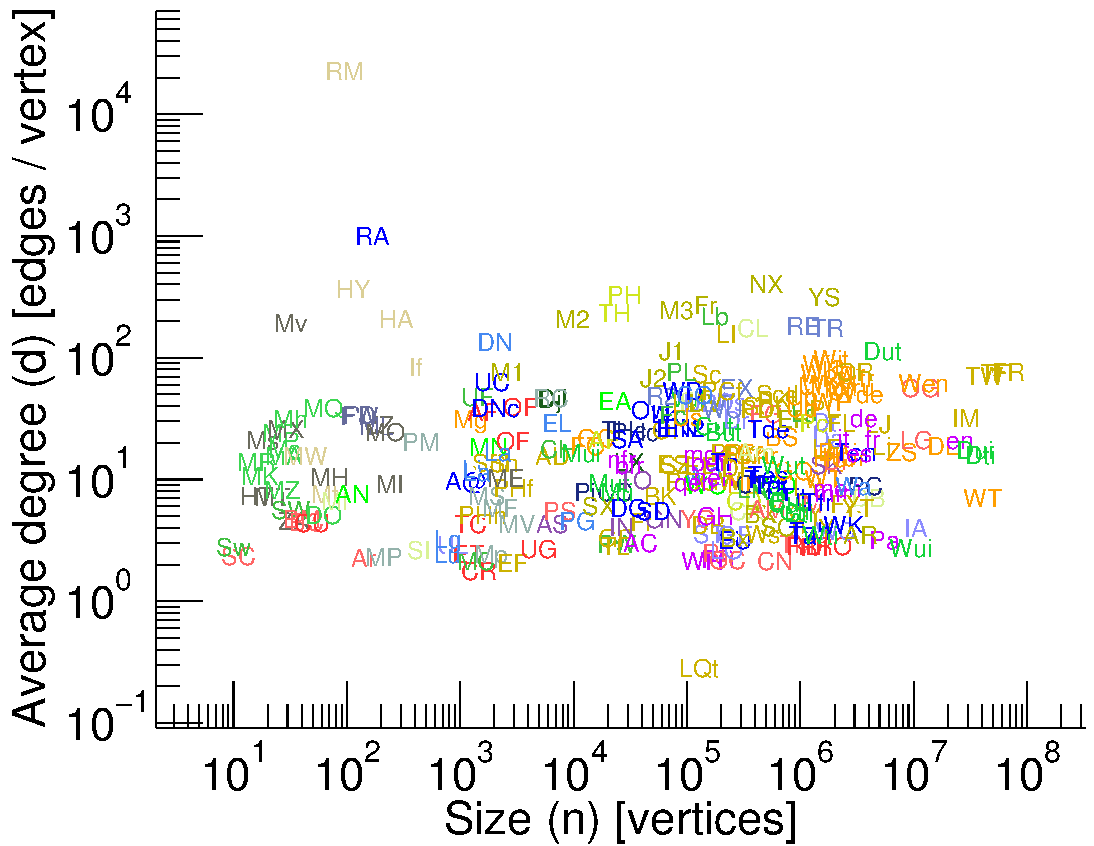
\includegraphics[width=0.8\textwidth]{plot/scatter.c.size.avgdegree.everything}
  \caption[*]{
    All networks in KONECT
    arranged by the size (the number of nodes) and the
    average number of neighbors of all nodes.  Each network is
    represented by a two- or three-character code. The color of each
    code corresponds to the network 
    category as given in Table~\ref{tab:categories}.  
  }
  \label{fig:scatter.size.avgdegree}
\end{figure}

\paragraph{Software and Software Packages}
The KONECT project consists of several components, whose interactions is
summarized in Figure~\ref{fig:organization}.  Various parts of the
KONECT project are available at Github, including this Handbook.\footnote{\href{https://github.com/kunegis/konect-analysis}{github.com/kunegis/konect-analysis}}\footnote{\href{https://github.com/kunegis/konect-toolbox}{github.com/kunegis/konect-toolbox}}\footnote{\href{https://github.com/kunegis/konect-handbook}{github.com/kunegis/konect-handbook}}\footnote{\href{https://github.com/kunegis/konect-extr}{github.com/kunegis/konect-extr}}

\begin{figure}
  \centering
  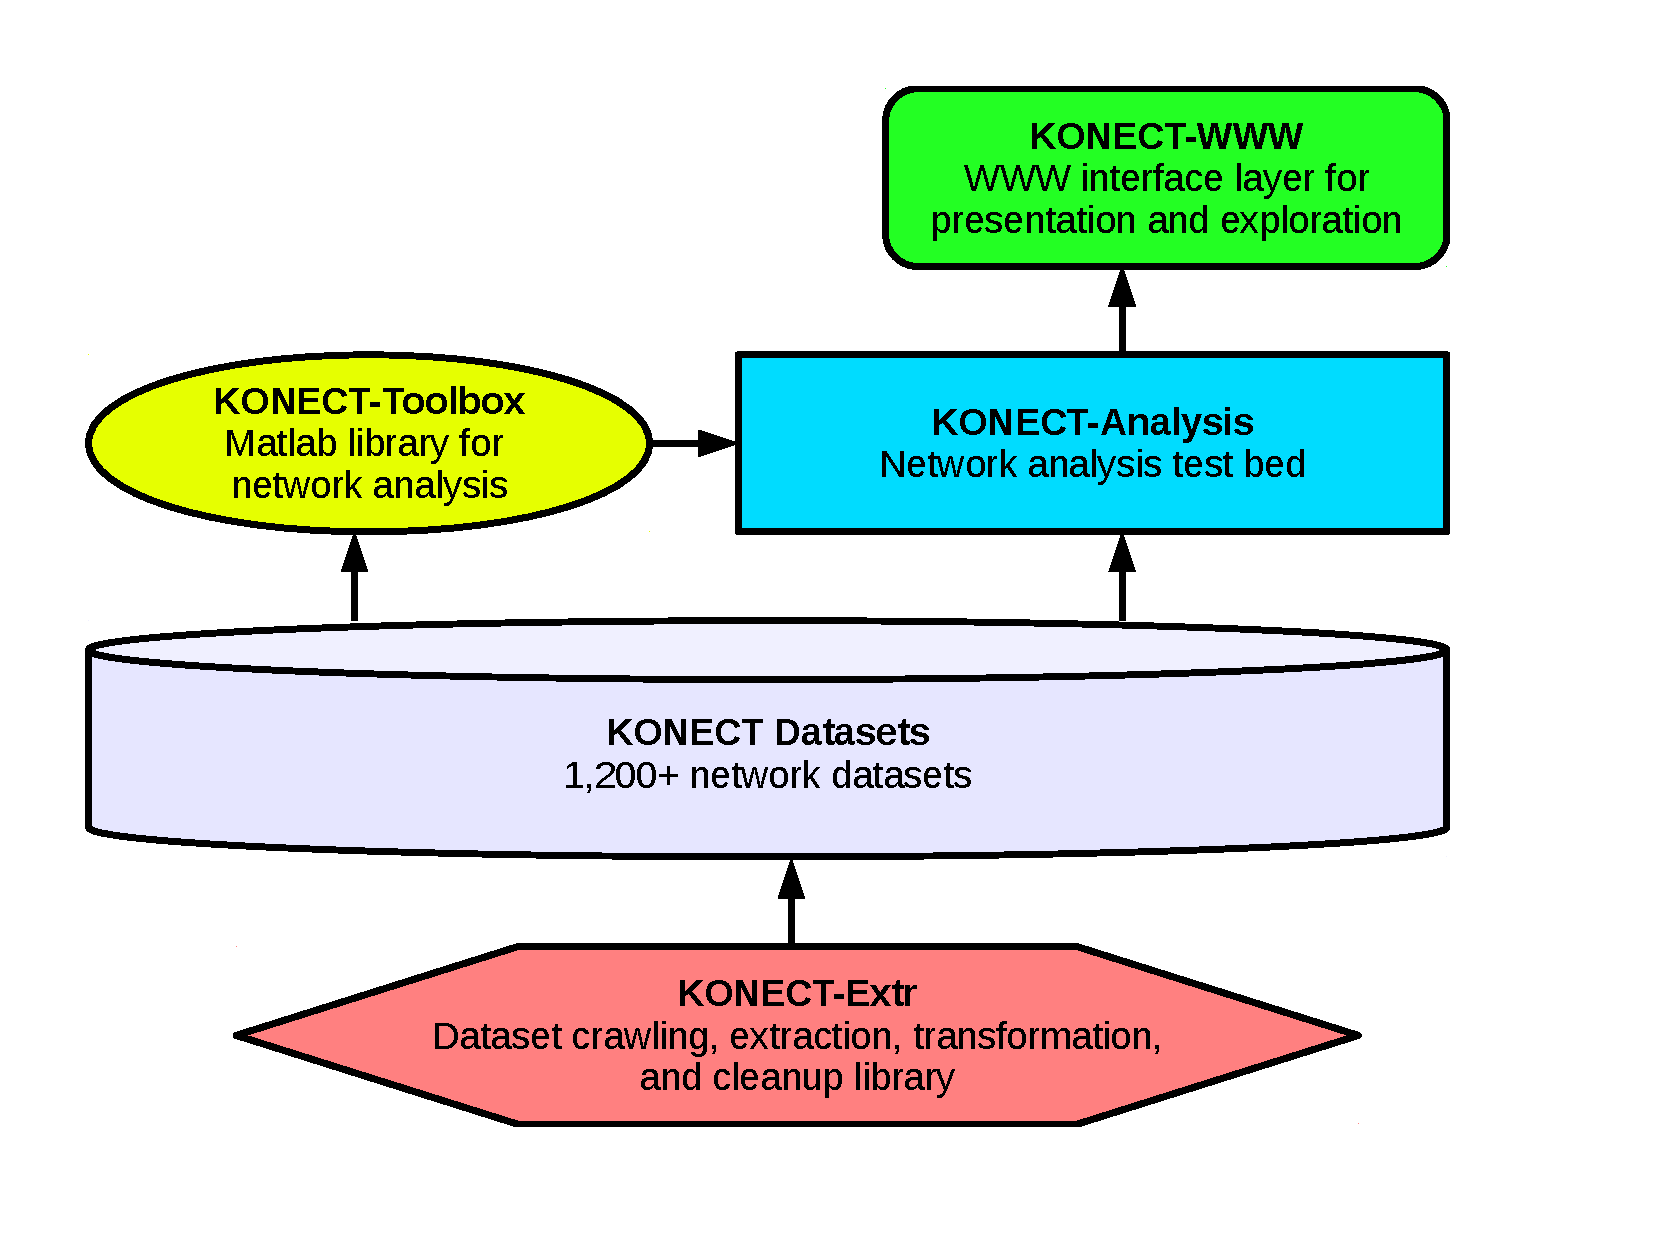
\includegraphics[width=\wOnePointFive]{organization.white}
  \caption{
    \label{fig:organization}
    Overview of KONECT's components. 
  }
\end{figure}

\paragraph{History of KONECT}
What later became known as the KONECT project started out in December 2008 at the Technical University of
Berlin's DAI Laboratory, as evaluation for Jérôme Kunegis' ICML 2009
paper \emph{Learning Spectral Graph Transformations for Link Prediction}
\citep{kunegis:spectral-transformation}, codenamed \emph{Spectral
  Transformation}.  It then consisted of a collection of network
datasets and spectral link prediction methods.  Later, more datasets
were added and the codebase was called the \emph{Graph Store}, and the
project was used for the experiments of several papers in the area of
collaborative filtering and recommender systems.  When Jérôme moved from
TU Berlin to the University of Koblenz--Landau in Koblenz (Germany) the
project was renamed \emph{Web Store}, in line with Koblenz' Institute
for Web Science and Technologies (WeST).  The name \emph{KONECT --
  Koblenz Network Collection} was adopted sometime in 2011.  The KONECT
website was created in 2011 under
\href{http://konect.uni-koblenz.de/}{\texttt{konect.uni-koblenz.de}}.
Code for dataset extraction and the Matlab Toolbox was first published
on the KONECT website.  A short overview paper of the KONECT system was
published in 2013 at the International World Wide Web Conference (WWW),
as part of the Web Observatory Workshop \citep{kunegis:konect}.  In 2015
and 2016, various parts of the KONECT project were placed on GitHub under the GNU
General Public License version 3, including this handbook.  From 2017
on, the KONECT project continued to be developed at the University of
Namur (Belgium), with web hosting provided by the Institute for Web
Science and Technologies (WeST) at the University of
Koblenz--Landau.

\paragraph{Structure of this Handbook}
This handbook serves both as a compendium of mathematical definitions
used in the KONECT project, as well as documentation of the software
used in KONECT. 
\begin{itemize}
\item Section \ref{sec:taxonomy} ``Networks'' gives the basic
  definition of a network as used in KONECT -- as networks exists in
  many different variants such as directed, bipartite, signed, etc., the
  exact definitions are often overlooked, but can be crucial for
  understanding individual relations. The taxonomy of networks given in
  this section serves for the rest of the project. 
\item Section \ref{sec:definitions} ``Graph Theory'' gives the
  graph-theoretical definitions underlying all topics of network analysis.  Again,
  the devil is in the details and the graph theory literature is often
  split between multiple incompatible definitions for commonly used
  terms.  This sections presents the terminology and definitions as used
  in KONECT, which represents a compromise that has been proven useful
  in practice. 
\item Section \ref{sec:statistics} ``Network Statistics'' is devoted to
  network statistics, i.e., numerical measures that characterize a
  network as a whole.  These are central to network analysis, and most
  common network statistics are covered. 
\item Section \ref{sec:features} ``Node Features'' covers node features,
  i.e., numerical measures that characterize individual nodes in a
  network.  These are often used as measures of centrality or
  importance, etc. 
\item Section \ref{sec:matrix} ``Graph Matrices and Decompositions'' reviews
  characteristic matrices used to analyse graphs, with a focus on their
  decompositions.  These are crucial in various types of analyses,
  include pairwise node measures such as distances and similarities, as
  well as node-based measures such as centralities. 
\item Section \ref{sec:plots} ``Network Plots'' reviews common ways to
  visualize properties of a network.  Some of those, such as the degree
  distribution, are ubiquitous in the literature. 
\item Section \ref{sec:toolbox} ``The KONECT Toolbox'' describes the GNU
  Octave and Matlab toolbox that is part of the KONECT project. 
\item Section \ref{sec:format} ``File Formats'' finally documents the
  file formats used by KONECT. 
\end{itemize}
\marginnote{
  \textlangle{}\texttt{name}\textrangle
}
Throughout the handbook, we will use margin notes to give the internal
names of various parameters. 

\section{Networks}
\label{sec:taxonomy}
Datasets in KONECT represent networks, i.e., a set of nodes connected by
links. Networks can be classified by their format
(directed/undirected/bipartite), by their edge weight types and
multiplicities, by the 
presence of metadata such as timestamps and node labels, and by
the types of objects represented by nodes and links. 
The full list of networks is given online.\footnote{\href{http://konect.uni-koblenz.de/networks/}{konect.uni-koblenz.de/networks}}

The format of a network is always one of the following.  The network
formats are summarized in Table~\ref{tab:format}. 
\begin{itemize}
\item 
  In \textbf{undirected networks} (U), 
  \marginnote{\texttt{sym}}
  edges are undirected.  That is,
  there is no difference between the edge from $u$ to $v$ and the edge
  from $v$ to $u$; both are the edge $\{u,v\}$. 
  An example of an undirected network is the social network of
  Facebook
  (\href{http://konect.uni-koblenz.de/networks/facebook-wosn-wall}{\textsf{Ow}}),
  in which there is no difference between the statements ``A 
  is a friend of B'' and ``B is a friend of A.''
\item In a \textbf{directed network} (D), 
  \marginnote{\texttt{asym}}
  the links are directed. That is, there is a
  difference between the edge $(u,v)$ and the edge $(u,v)$. 
  Directed networks are sometimes also called \emph{digraphs} (for \emph{directed
    graphs}), and their edges \emph{arcs}. 
  An example of a directed social network is the follower network of
  Twitter
  (\href{http://konect.uni-koblenz.de/networks/twitter_mpi}{\textsf{TF}}),
  in which the fact that user A follows user B does not imply 
  that user B follows user A. 
\item \textbf{Bipartite networks} (B) 
  \marginnote{\texttt{bip}}
  include two types of nodes, and all edges
  connect one node type with the other. An example of a bipartite
  network is a rating graph, consisting of the node types \emph{user}
  and \emph{movie}, and each rating connects a user and a movie
  (\href{http://konect.uni-koblenz.de/networks/movielens-10m_rating}{\textsf{M3}}).  
  Bipartite networks are always undirected in KONECT. 
\end{itemize}

\begin{table}
  \caption{
    The network formats allowed in KONECT.
    Each network dataset is exactly of one type.  
    \label{tab:format}
  }
  \centering
\makebox[\textwidth]{
  \begin{tabular}{ c l llll }
    \toprule
    \textbf{\#} & \textbf{Symbol} & \textbf{Type} & \textbf{Edge partition} & \textbf{Edge types} & \textbf{Internal name} \\
    \midrule
    1 & U & Undirected	& Unipartite	& Undirected	& \texttt{sym}  \\
    2 & D & Directed	& Unipartite	& Directed	& \texttt{asym} \\
    3 & B & Bipartite	& Bipartite	& Undirected	& \texttt{bip}  \\
    \bottomrule
  \end{tabular}
}
\end{table}

The edge weight and multiplicity types of networks are represented by
one of the following eight types. 
The types of edge weights and multiplicities are summarized in
Table~\ref{tab:weights}. 
\begin{itemize}
\item An \textbf{unweighted network} ($-$) 
  \marginnote{\texttt{unweighted}}
  has edges that are
  unweighted, and only a 
  single edge is allowed between any two nodes.  
\item In a \textbf{network with multiple edges} ($=$), 
  \marginnote{\texttt{positive}}
  two nodes can be
  connected by any number of edges, and all edges are unweighted. This
  type of network is also called a multigraph.  
\item In a \textbf{positive network} ($+$), 
  \marginnote{\texttt{posweighted}}
  edges are annotated
  with positive weights, and only a single edge is allowed between
  any node pair.  The weight zero identified with the lack of an edge
  and thus, we require that each edge has a weight strictly larger than
  zero. 
\item In a \textbf{signed network} ($\pm$), 
  \marginnote{\texttt{signed}}
  both positive and negative
  edges are 
  allowed. Positive and negative edges are represented by positive and
  negative edge weights. Many networks of this type have only the
  weights $\pm 1$, but in the general case we allow any nonzero weight.
\item \textbf{Networks with multiple signed edges} ($\stackrel{+}{=}$) 
  \marginnote{\texttt{multisigned}}
  allow multiple edges between two nodes, which may have the same values
  as edges in a signed network.
\item \textbf{Rating networks} ($*$) 
  \marginnote{\texttt{weighted}}
  have arbitrary real edge weights.  They
  differ from positive and signed networks in that the edge weights are
  interpreted as an interval scale, and thus the value zero has no
  special meaning.  Adding a constant to all edge weights does not
  change the semantics of a rating network. 
  Ratings can be discrete, such as the one-to-five star ratings, or
  continuous, such as a rating given in percent. 
  This type of network allows only a single edge between two nodes. 
\item \textbf{Networks with multiple ratings} ($_*{}^*$) 
  \marginnote{\texttt{multiweighted}}
  have edges annotated
  with rating values, and allow multiple edges between two nodes.
\item \textbf{Dynamic networks} ($\rightleftarrows$) are networks in
  \marginnote{\texttt{dynamic}}
  which edges can appear and disappear.  They are always
  temporal. Individual edges are not weighted. 
\end{itemize}

Metadata of networks are further properties that go beyond the formats
and weights listed above. 
\begin{itemize}
\item \textbf{Temporal networks} (\Clocklogo) include a timestamp for each
  edge, and thus the network can be reconstructed for any moment in the
  past. 
\item \textbf{Networks with loops} ($\circlearrowright$) are unipartite networks in
  which edges of the form $\{u,u\}$ are allowed, i.e., edges connecting
  a node with itself. 
\end{itemize}

\begin{table}
  \caption{
    The edge weight and multiplicity types allowed in KONECT. Each
    network dataset is exactly of one type. 
    Note that due to historical reasons, networks with multiple
    unweighted edges have the internal name \texttt{positive}, while
    positively weighted networks have the internal
    \texttt{posweighted}. 
    For signed networks and positive edge weights, weights of zero are
    only allowed when the tag \texttt{\#zeroweight} is set. 
    \label{tab:weights}
  }
  \centering
\makebox[\textwidth]{
  \begin{tabular}{cllllll}
    \toprule
    \textbf{\#} & \textbf{Symbol} &\textbf{Type} & \textbf{Multiple} & \textbf{Edge weight} &
    \textbf{Edge weight} &
    \textbf{Internal name} \\ 
    & & & \textbf{edges} & \textbf{range} & \textbf{scale}  \\
    \midrule
    1 & $-$   & Unweighted          & No  & $\{1\}$        & --    & \texttt{unweighted} \\
    2 & $=$   & Multiple unweighted & Yes & $\{1\}$         &  --  & \texttt{positive}   \\
    3 & $+$   & Positive weights    & No  & $(0, \infty)$      & Ratio scale     & \texttt{posweighted}\\
    4 & $\pm$ & Signed              & No  & $(-\infty,+\infty)$ & Ratio scale    & \texttt{signed}     \\
    5 & $\stackrel{+}{=}$ & Multiple signed  & Yes & $(-\infty,+\infty)$ & Ratio scale    & \texttt{multisigned} \\
    6 & $*$   & Rating              & No  & $(-\infty,+\infty)$ &Interval scale  & \texttt{weighted}   \\
    7 & $_*{}^*$ & Multiple ratings & Yes & $(-\infty,+\infty)$ & Interval scale  & \texttt{multiweighted}\\
    8 & $\rightleftarrows$ & Dynamic & Yes & $\{1\}$            & --	     & \texttt{dynamic}      \\
    9 &  & Multiple positive weights & Yes & $(0, \infty)$      & Ratio scale & \texttt{multiposweighted} \\
    \bottomrule
  \end{tabular}
  }
\end{table}

Finally, the network categories classify networks by the type of data they
represent.  
An overview of the categories is given in Table~\ref{tab:categories}. 

\begin{table*}
  \caption{
    The network categories in KONECT.  
    Each category is assigned a color, which is used in plots, for
    instance in Figure~\ref{fig:scatter.size.avgdegree}. The property
    symbols are defined in Table \ref{tab:weights}.  U: Undirected
    network, D: Directed network, B: Bipartite network. 
    \label{tab:categories}
  }
  \centering
\makebox[\textwidth]{
  \begin{tabular}{lllllr}
\toprule
& \textbf{Internal name} & \textbf{Vertices} & \textbf{Edges} & \textbf{Properties} & \textbf{Count} \\
\midrule
\textcolor{colorAffiliation}{$\newmoon$} &\texttt{Affiliation} & Actors, groups & Membership & \phantom{U} \phantom{D} B $-$ $=$ \phantom{$+$} \phantom{$\pm$} \phantom{$\stackrel{+}{=}$} \phantom{$*$} \phantom{$_*{}^*$} \phantom{$\rightleftharpoons$} \phantom{$++$}  &  16\\
\textcolor{colorAnimal}{$\newmoon$} &\texttt{Animal} & Animals & Tie & U D \phantom{B} $-$ \phantom{$=$} $+$ \phantom{$\pm$} \phantom{$\stackrel{+}{=}$} \phantom{$*$} \phantom{$_*{}^*$} \phantom{$\rightleftharpoons$} \phantom{$++$}  &  9\\
\textcolor{colorAuthorship}{$\newmoon$} &\texttt{Authorship} & Authors, works & Authorship & \phantom{U} \phantom{D} B $-$ $=$ \phantom{$+$} \phantom{$\pm$} \phantom{$\stackrel{+}{=}$} \phantom{$*$} \phantom{$_*{}^*$} \phantom{$\rightleftharpoons$} \phantom{$++$}  &  808\\
\textcolor{colorCitation}{$\newmoon$} &\texttt{Citation} & Documents & Citation & \phantom{U} D \phantom{B} $-$ \phantom{$=$} \phantom{$+$} \phantom{$\pm$} \phantom{$\stackrel{+}{=}$} \phantom{$*$} \phantom{$_*{}^*$} \phantom{$\rightleftharpoons$} \phantom{$++$}  &  7\\
\textcolor{colorCoauthorship}{$\newmoon$} &\texttt{Coauthorship} & Authors & Coauthorship & U \phantom{D} \phantom{B} $-$ $=$ \phantom{$+$} \phantom{$\pm$} \phantom{$\stackrel{+}{=}$} \phantom{$*$} \phantom{$_*{}^*$} \phantom{$\rightleftharpoons$} \phantom{$++$}  &  3\\
\textcolor{colorCocitation}{$\newmoon$} &\texttt{Cocitation} & Authors & Cocitation & U \phantom{D} \phantom{B} \phantom{$-$} $=$ \phantom{$+$} \phantom{$\pm$} \phantom{$\stackrel{+}{=}$} \phantom{$*$} \phantom{$_*{}^*$} \phantom{$\rightleftharpoons$} \phantom{$++$}  &  2\\
\textcolor{colorCommunication}{$\newmoon$} &\texttt{Communication} & Persons & Message & U D \phantom{B} $-$ $=$ \phantom{$+$} \phantom{$\pm$} \phantom{$\stackrel{+}{=}$} \phantom{$*$} \phantom{$_*{}^*$} \phantom{$\rightleftharpoons$} \phantom{$++$}  &  42\\
\textcolor{colorComputer}{$\newmoon$} &\texttt{Computer} & Computers & Connection & U D \phantom{B} $-$ $=$ \phantom{$+$} \phantom{$\pm$} \phantom{$\stackrel{+}{=}$} \phantom{$*$} \phantom{$_*{}^*$} \phantom{$\rightleftharpoons$} \phantom{$++$}  &  13\\
\textcolor{colorFeature}{$\newmoon$} &\texttt{Feature} & Items, features & Property & \phantom{U} \phantom{D} B $-$ $=$ $+$ \phantom{$\pm$} \phantom{$\stackrel{+}{=}$} \phantom{$*$} \phantom{$_*{}^*$} \phantom{$\rightleftharpoons$} \phantom{$++$}  &  17\\
\textcolor{colorHumanContact}{$\newmoon$} &\texttt{HumanContact} & Persons & Real-life contact & U \phantom{D} \phantom{B} \phantom{$-$} $=$ $+$ \phantom{$\pm$} \phantom{$\stackrel{+}{=}$} \phantom{$*$} \phantom{$_*{}^*$} \phantom{$\rightleftharpoons$} \phantom{$++$}  &  5\\
\textcolor{colorHumanSocial}{$\newmoon$} &\texttt{HumanSocial} & Persons & Real-life tie & U D \phantom{B} $-$ \phantom{$=$} $+$ $\pm$ $\stackrel{+}{=}$ \phantom{$*$} \phantom{$_*{}^*$} \phantom{$\rightleftharpoons$} \phantom{$++$}  &  12\\
\textcolor{colorHyperlink}{$\newmoon$} &\texttt{Hyperlink} & Web page & Hyperlink & \phantom{U} D B $-$ $=$ \phantom{$+$} \phantom{$\pm$} \phantom{$\stackrel{+}{=}$} \phantom{$*$} \phantom{$_*{}^*$} $\rightleftharpoons$ \phantom{$++$}  &  191\\
\textcolor{colorInfrastructure}{$\newmoon$} &\texttt{Infrastructure} & Location & Connection & U D \phantom{B} $-$ $=$ $+$ \phantom{$\pm$} \phantom{$\stackrel{+}{=}$} \phantom{$*$} \phantom{$_*{}^*$} \phantom{$\rightleftharpoons$} \phantom{$++$}  &  23\\
\textcolor{colorInteraction}{$\newmoon$} &\texttt{Interaction} & Persons, items & Interaction & \phantom{U} D B $-$ $=$ \phantom{$+$} \phantom{$\pm$} $\stackrel{+}{=}$ \phantom{$*$} \phantom{$_*{}^*$} \phantom{$\rightleftharpoons$} \phantom{$++$}  &  25\\
\textcolor{colorLexical}{$\newmoon$} &\texttt{Lexical} & Words & Lexical relationship & U D \phantom{B} $-$ $=$ \phantom{$+$} \phantom{$\pm$} \phantom{$\stackrel{+}{=}$} \phantom{$*$} \phantom{$_*{}^*$} \phantom{$\rightleftharpoons$} \phantom{$++$}  &  5\\
\textcolor{colorMetabolic}{$\newmoon$} &\texttt{Metabolic} & Metabolites & Interaction & U D \phantom{B} $-$ $=$ \phantom{$+$} \phantom{$\pm$} \phantom{$\stackrel{+}{=}$} \phantom{$*$} \phantom{$_*{}^*$} \phantom{$\rightleftharpoons$} \phantom{$++$}  &  7\\
\textcolor{colorMisc}{$\newmoon$} &\texttt{Misc} & Various & Various & U D \phantom{B} $-$ $=$ $+$ \phantom{$\pm$} \phantom{$\stackrel{+}{=}$} \phantom{$*$} \phantom{$_*{}^*$} \phantom{$\rightleftharpoons$} \phantom{$++$}  &  11\\
\textcolor{colorOnlineContact}{$\newmoon$} &\texttt{OnlineContact} & Users & Online interaction & U D \phantom{B} $-$ $=$ \phantom{$+$} $\pm$ $\stackrel{+}{=}$ \phantom{$*$} \phantom{$_*{}^*$} $\rightleftharpoons$ \phantom{$++$}  &  15\\
\textcolor{colorRating}{$\newmoon$} &\texttt{Rating} & Users, items & Rating & \phantom{U} \phantom{D} B $-$ $=$ \phantom{$+$} \phantom{$\pm$} \phantom{$\stackrel{+}{=}$} $*$ $_*{}^*$ \phantom{$\rightleftharpoons$} \phantom{$++$}  &  15\\
\textcolor{colorSocial}{$\newmoon$} &\texttt{Social} & Persons & Online tie & U D \phantom{B} $-$ \phantom{$=$} $+$ $\pm$ \phantom{$\stackrel{+}{=}$} $*$ \phantom{$_*{}^*$} $\rightleftharpoons$ \phantom{$++$}  &  46\\
\textcolor{colorSoftware}{$\newmoon$} &\texttt{Software} & Software Component & Dependency & \phantom{U} D \phantom{B} $-$ $=$ \phantom{$+$} \phantom{$\pm$} \phantom{$\stackrel{+}{=}$} \phantom{$*$} \phantom{$_*{}^*$} \phantom{$\rightleftharpoons$} \phantom{$++$}  &  3\\
\textcolor{colorText}{$\newmoon$} &\texttt{Text} & Documents, words & Occurrence & \phantom{U} \phantom{D} B \phantom{$-$} $=$ \phantom{$+$} \phantom{$\pm$} \phantom{$\stackrel{+}{=}$} \phantom{$*$} \phantom{$_*{}^*$} \phantom{$\rightleftharpoons$} \phantom{$++$}  &  10\\
\textcolor{colorTrophic}{$\newmoon$} &\texttt{Trophic} & Species & Carbon exchange & \phantom{U} D \phantom{B} $-$ \phantom{$=$} $+$ \phantom{$\pm$} \phantom{$\stackrel{+}{=}$} \phantom{$*$} \phantom{$_*{}^*$} \phantom{$\rightleftharpoons$} \phantom{$++$}  &  3\\
\midrule
& \textbf{Total} &&&& \textbf{1288}\\
\bottomrule
\end{tabular}

}
\end{table*}

\begin{description}
\item[Affiliation networks] are bipartite networks denoting the
  \marginnote{\texttt{Affiliation}}
  membership of actors in groups.  Groups can be defined as narrowly as
  individual online communities in which users have been active
  (\href{http://konect.uni-koblenz.de/networks/flickr-groupmemberships}{\textsf{FG}})
  or as broadly as countries
  (\href{http://konect.uni-koblenz.de/networks/dbpedia-country}{\textsf{CN}}). The
  actors are mainly persons, but can also be other actors such as musical
  groups. Note that in all affiliation networks we consider, each actor
  can be in more than one group, as otherwise the network cannot be
  connected.

\item[Animal networks] are networks of contacts between animals.  
  \marginnote{\texttt{Animal}}
  They are the animal equivalent to human social networks.  Note that
  datasets of websites such as Dogster
  (\href{http://konect.uni-koblenz.de/networks/petster-friendships-dog}{\textsf{Sd}})
  are \emph{not} included here but in the \texttt{Social} (online social
  network) category, since the networks are generated by humans. 

\item[Authorship networks] are unweighted bipartite networks consisting
  \marginnote{\texttt{Authorship}}
  of links between authors and their works.  In some authorship networks
  such as that of scientific literature
  (\href{http://konect.uni-koblenz.de/networks/dblp-author}{\textsf{Pa}}),
  works have typically only few authors, whereas works in other
  authorship networks may have many authors, as in Wikipedia articles
    (\href{http://konect.uni-koblenz.de/networks/edit-enwiki}{\textsf{en}}).

\item[Citation networks] consist of documents that reference each
  \marginnote{\texttt{Citation}}
  other.  The primary example are scientific publications, but the
  category also allow patents and other types of documents that
  reference each other. 

\item[Coauthorship networks] are unipartite network connecting authors
  \marginnote[\texttt{Coauthorship}]
  who have written works together, for instance academic literature, but
  also other types of works such as music or movies. 

\item[Communication networks] contain edges that represent
  \marginnote{\texttt{Communication}}
  individual messages between persons.  Communication networks are directed
  and allow multiple edges.  
  Examples of communication networks are those of
  emails (\href{http://konect.uni-koblenz.de/networks/enron}{\textsf{EN}})
  and those of
  Facebook messages
  (\href{http://konect.uni-koblenz.de/networks/facebook-wosn-wall}{\textsf{Ow}}). Note
  that in some instances, edge directions are not 
  known and KONECT can only provide an undirected network. 

\item[Computer networks] are networks of connected computers. 
  \marginnote{\texttt{Computer}}
  Nodes in them are computers, and edges are connections. 
  When speaking about \emph{networks} in a computer science context, one
  often means only computer networks.  An example is the internet
  topology network (\href{http://konect.uni-koblenz.de/networks/topology}{\textsf{TO}}).

\item[Feature networks] are bipartite, and denote any kind of feature
  \marginnote{\texttt{Feature}}
  assigned to entities. Feature networks are unweighted and have
  edges that are not annotated with edge creation times.  Examples are
  songs and their genres
  (\href{http://konect.uni-koblenz.de/networks/dbpedia-genre}{\textsf{GE}}).   

\item[Folksonomies] consist of tag assignments connecting a user, an
  \marginnote{\texttt{Folksonomy}}
  item and a tag.  For folksonomies, we follow the 3-bipartite
  projection approach and consider the three possible bipartite
  networks, i.e., the user--item, user--tag and item--tag networks.
  This allows us to apply methods for bipartite graphs to hypergraphs,
  which is not possible otherwise.  Items that are tagged in
  folksonomies include bookmarks
  (\href{http://konect.uni-koblenz.de/networks/delicious-ui}{\textsf{Dui}}),
  scientific publications
  (\href{http://konect.uni-koblenz.de/networks/citeulike-ui}{\textsf{Cui}})
  and movies
  (\href{http://konect.uni-koblenz.de/networks/movielens-10m_ui}{\textsf{Mui}}).

\item[Human contact networks] are unipartite networks of actual contact
  \marginnote{\texttt{HumanContact}}
  between persons, i.e., talking with each other, spending time
  together, or at least being physically close.  Usually, these datasets
  are collected by giving out RFID tags to people with chips that record
  which other people are in the vicinity.  Determining when an actual
  contact has happened (as opposed to for instance to persons standing
  back to back) is a nontrivial research problem. 
  An example is the Reality Mining dataset
  (\href{http://konect.uni-koblenz.de/networks/mit}{\textsf{RM}}). 

\item[Human social networks] are real-world social networks between
  humans.  
  \marginnote{\texttt{HumanSocial}}
  The ties must be offline, and not from an online social network.
  Also, the ties represent a state, as opposed to human contact
  networks, in which each edge represents an event. 

\item[Hyperlink networks] are the networks of web pages connected by
  hyperlinks.  

\item[Infrastructure networks] are networks of physical infrastructure.  
  \marginnote{\texttt{Infrastructure}}
  Examples are road networks
  (\href{http://konect.uni-koblenz.de/networks/roadNet-CA}{RO}), airline
  connection networks
  (\href{http://konect.uni-koblenz.de/networks/opsahl-openflights}{OF}), 
  and power grids
  (\href{http://konect.uni-koblenz.de/networks/opsahl-powergrid}{UG}).  
  
\item[Interaction networks] are bipartite networks consisting of people
  \marginnote{\texttt{Interaction}}
  and items, where each edge represents an interaction. 
  In interaction networks, we always allow multiple edges between the
  same person--item pair.
  Examples are
  people writing in forums
  (\href{http://konect.uni-koblenz.de/networks/opsahl-ucforum}{\textsf{UF}}),
  commenting on movies
  (\href{http://konect.uni-koblenz.de/networks/filmtipset_comment}{\textsf{Fc}}),
  listening to songs
  (\href{http://konect.uni-koblenz.de/networks/lastfm_song}{\textsf{Ls}})
  and sports results. 

\item[Lexical networks] consist of words from natural 
  \marginnote{\texttt{Lexical}}
  languages and the
  relationships between them. 
  Relationships can be semantic (i.e, related to the
  meaning of words) such as the
  synonym
    relationship (\href{http://konect.uni-koblenz.de/networks/wordnet-words}{\textsf{WO}}), associative such
  as when two words are associated with each other by people in
  experiments (\href{http://konect.uni-koblenz.de/networks/eat}{\textsf{EA}}), or denote 
  cooccurrence, i.e., the fact that two words co-occur in text (\href{http://konect.uni-koblenz.de/networks/lasagne-spanishbook}{\textsf{SB}}).  Note
  that lexical cooccurrence networks are explicitly not included in the
  broader Cooccurrence category. 

\item[Metabolic networks] model metabolic pathways. 
  \marginnote{\texttt{Metabolic}}

\item[Miscellaneous networks] are any networks that do not fit into one
  \marginnote{\texttt{Misc}}
  of the other categories. 
  
\item[Online Contact networks] consist of people and interactions between
  \marginnote{\texttt{OnlineContact}}
  them. 
  Contact networks are unipartite and allow multiple edges, i.e., there
  can always be multiple interactions between the same two persons.
  They can be both directed or undirected.
  Examples are people that meet each other
  (\href{http://konect.uni-koblenz.de/networks/mit}{\textsf{RM}}), or
  scientists that write a paper together
  (\href{http://konect.uni-koblenz.de/networks/dblp_coauthor}{\textsf{Pc}}).

\item[Physical networks] represent physically existing network
  \marginnote{\texttt{Physical}}
  structures in the broadest sense.  This category covers such diverse data as
  physical computer networks
  (\href{http://konect.uni-koblenz.de/networks/topology}{\textsf{TO}}),
  transport networks
  (\href{http://konect.uni-koblenz.de/networks/opsahl-openflights}{\textsf{OF}})
  and biological food networks
  (\href{http://konect.uni-koblenz.de/networks/foodweb-baydry}{\textsf{FD}}).   

\item[Rating networks] consist of assessments given to items by users,
  \marginnote{\texttt{Rating}}
  weighted by a rating value.  Rating networks are bipartite.  
  Networks in which users can rate other users are not included here,
  but in the Social category instead.  If only a single type of rating
  is possible, for instance the ``favorite'' relationship, then rating
  networks are unweighted.  Examples of items that are rated are movies
  (\href{http://konect.uni-koblenz.de/networks/movielens-10m_rating}{\textsf{M3}}), 
  songs
  (\href{http://konect.uni-koblenz.de/networks/yahoo-song}{\textsf{YS}}),
  jokes
  (\href{http://konect.uni-koblenz.de/networks/jester}{\textsf{JE}}),
  and even sexual escorts
  (\href{http://konect.uni-koblenz.de/networks/escorts}{\textsf{SX}}).   

\item[Online social networks] represent ties between
  \marginnote{\texttt{Social}}
  persons in online social networking platforms.  Certain social
  networks allow negative edges, which denote 
  enmity, distrust or dislike.
  Examples are Facebook friendships
  (\href{http://konect.uni-koblenz.de/networks/facebook-sg}{\textsf{FSG}}),
  the Twitter follower relationship
  (\href{http://konect.uni-koblenz.de/networks/twitter_mpi}{\textsf{TF}}), 
  and friends and foes on Slashdot
  (\href{http://konect.uni-koblenz.de/networks/slashdot-zoo}{\textsf{SZ}}).  
  Note that some social networks can be argued to be rating networks,
  for instance the 
  user--user rating network of a dating site
  (\href{http://konect.uni-koblenz.de/networks/libimseti}{\textsf{LI}}). 
  These networks are all included in the Social category. 

\item[Software networks] are networks of interacting software
  \marginnote{\texttt{Software}}
  component.  Node can be software packages connected by their
  dependencies, source files connected by includes, and classes
  connected by imports. 

\item[Text networks] consist of text documents containing words.  They
  \marginnote{\texttt{Text}}
  are bipartite and their nodes are documents and words.  Each edge
  represents the occurrence of a word in a document. Document types are
  for instance
  newspaper articles
  (\href{http://konect.uni-koblenz.de/networks/gottron-trec}{\textsf{TR}})
  and Wikipedia articles
  (\href{http://konect.uni-koblenz.de/networks/gottron-excellent}{\textsf{EX}}). 

\item[Trophic networks] consist of biological species connected by edges denotes
  \marginnote{\texttt{Trophic}}
  which pairs of species are subject to carbon exchange, i.e., which
  species eats which.  The term \emph{food chain} describes such
  relation ships, but note that in the general case, a trophic network
  is not a chain, i.e., it is not linear.  Trophic networks are
  directed. 

\end{description}

Note that the category system of KONECT is in flux.  As networks are
added to the collection, large categories are split into smaller ones. 

We do not include certain kinds of networks that lack a complex
structure. This includes networks without a giant connected component,
in which most nodes are not reachable from each other, and trees, in
which there is only a single path between any two nodes.  Note that
bipartite relationships extracted from n-to-1 relationships are
therefore excluded, as they lead to a disjoint network. For instance, a
bipartite person--city network containing \emph{was-born-in} edges would
not be included, as each city would form its own component disconnected
from the rest of the network.  On the other hand, a band--country
network where edges denote the country of origin of individual band
members is included, as members of a single band can have different
countries of origin. In fact the Countries network
(\href{http://konect.uni-koblenz.de/networks/dbpedia-country}{\textsf{CN}})
is of this form.  Another example is a bipartite song--genre network,
which would only be included in KONECT when songs can have multiple
genres.  As an example of the lack of complex structure when only a
single genre is allowed, the degree distribution in such a song--genre
network is skewed because all song nodes have degree one, the diameter
cannot be computed since the network is disconnected, and each connected
component trivially has a diameter of two or less.

\subsection{Tags}
\label{sec:tags}
The following tags can be given to networks.  They are declared in the
\texttt{tags} field in the \texttt{meta.*} file for each network. 
\begin{itemize}
\item \texttt{\#acyclic}:  The network is acyclic.  Can only be
  set for directed networks.  If this is not set, a directed
  network must contain at least two pairs of reciprocal edges of
  the form $(u,v)$ and $(v,u)$.  If the network does not contain
  reciprocal edges, but has cycles, the tag
  \texttt{\#nonreciprocal} is used.
\item \texttt{\#aggregatetime}:  The small value of timestamps
  stand for any earlier time; these timestamps should not be
  considered when performing time-based methods and plots. 
\item \texttt{\#incomplete}: The network is incomplete, i.e.,
  not all edges or nodes are included.  This implies that
  strictly speaking, certain statistics or plots like 
  the degree distribution are not meaningful, since they may
  depend on which parts are missing.  In practice, many datasets
  fall into this category, and they are not always excluded. 
\item \texttt{\#join}:  The network is actually the join of more
  fundamental networks.  For instance, a co-authorship network
  is a join of the authorship network with itself.  Networks
  that have this tag may have skewed properties, such as skewed
  degree distributions.
\item \texttt{\#kcore}: The network contains only nodes with a
  certain minimal degree $k$. In other words, the nodes with
  degree less than a certain number $k$ were removed from the
  dataset.  This changes a network drastically, and is called
  the ``$k$-core'' of a network. This is sometimes done to get
  a less sparse network in applications that do not perform well
  on sparse networks. This tag implies the
  \texttt{\#incomplete} tag.
\item \texttt{\#lowmultiplicity}:  Set in networks with multiple
  edges in which the actual maximal edge multiplicity is very
  low.  Used to be able to use the maximal multiplicity as a
  sanity check.  Indicates a dataset error, as edge
  multiplicities usually have a power law-like distribution, and
  thus very high edge multiplicities are usually present. 
\item \texttt{\#missingmultiplicity}:  This tag is used when the
  underlying network had inherent multiple edges, but these are
  not present in the dataset.  For instance, any email network
  that does not contain multiple edges is tagged with this. 
\item \texttt{\#missingorientation}: This tag is used for
  undirected networks which are based on an underlying
  directed network.  For instance, in a citation network, we
  may only know that the documents A and B are linked, but not
  which one cites the other.  In such a case, the network in
  KONECT is undirected, although the underlying network is
  actually directed.
\item \texttt{\#lcc}:  The dataset actually contains only the
  largest connected component of the actual network.  Implies
  \texttt{\#incomplete}.  This tag is not used when the network
  is connected for other reasons. 
\item \texttt{\#loop}: The network may contain loops, i.e.,
  egdes connecting a vertex to itself.  This tag is only
  allowed for unipartite networks.  When this tag is not
  present, loops are not allowed, and the presence of loops
  will be considered an error by analysis code.
\item \texttt{\#nonreciprocal}:  For directed networks only.
  The network does not contain reciprocal edges.  This is only
  used when the network is non-reciprocal, but does contain
  directed cycles.  If the network is acyclic,
  \texttt{\#acyclic} is used. 
\item \texttt{\#regenerate}: The network can be regenerated
  periodically and may be updated when a more recent dataset
  becomes available.
\item \texttt{\#tournament}:  The graph is directed and for each
  pair of nodes $\{u,v\}$, either the directed edge $u \rightarrow v$ or
  the directed edge $v \rightarrow u$ exists, but not both.  It
  is an error for a non-directed graph to have this tag.  If
  \texttt{\#tournament} is defined, then
  \texttt{\#nonreciprocal} must also be defined.  Also, the graph must
  not contain loops, and thus
  \texttt{\#loop} must not be defined. 
\item \texttt{\#zeroweight}:  Must be set if it is allowed for edge
  weights to be zero. Only used for networks with positive edge
  weights and signed/multisigned networks. 
\end{itemize}

\section{Graph Theory}
\label{sec:definitions}
The areas of graph theory and network analysis are young, and
many concepts within them notoriously lack a single established notation.  The
notation chosen in KONECT represents a compromise between familiarity
with the most common conventions, and the need to use an unambigous
choice of letters and symbols.  This section gives an overview of the
basic definitions used within KONECT, including in the rest of this handbook. 

\subsection{Graphs}
Graphs will be denoted as $G=(V,E)$, in which $V$ is the set of
vertices, and $E$ is the set of edges \citep{b116}. Without loss of
generality, we assume that the vertices $V$ are consecutive natural
numbers starting at one, i.e.,
\begin{align}
  V &= \{ 1, 2, 3, \dotsc, |V| \}.
\end{align}
Edges $e\in E$ will be denoted as sets of two vertices, i.e.,
$e=\{u,v\}$.  We say that two vertices are adjacent if they are
connected by an edge; this will be written as $u \leftrightarrow v$, and is equivalent to $\{u,v\}\in E$. 
For directed networks, $u \rightarrow v$ will denote the existence of a
directed edge from $u$ to $v$, and $u \rightleftarrows v$ will denote
that two directed edges of opposite orientation exist between $u$ and $v$.
We say that an
edge is incident to a vertex if the edge touches the vertex. Strictly
speaking, an edge $e$ is incident to node $u$ when $u\in e$, but this
notation may confusing and we avoid it. 

We also allow loops, i.e., edges of the form $\{u,u\}=\{u\}$.  Loops
appear for instance in email networks, where it is possible to send an
email to oneself, and therefore an edge may connect a vertex with
itself.  Most networks however do not contain loops, and therefore
networks that allow loops are annotated in KONECT with the 
\texttt{\#loop} tag, as described in Section~\ref{sec:format}. 

Most of the time, we work with only one given graph, and therefore it is
unambigous with node and edge set are meant by $V$ and $E$.  When
ambiguity is possible, we will use the notation
$V[G]$ and $E[G]$ to denote the vertex and edge sets of a graph $G$.
This notation using brackets may occasionally be extended to other graph
characteristics. 

In directed networks, edges are pairs instead of sets, i.e.,
$e=(u,v)$.  In this case, we have $(u,v)\neq(v,u)$ whenever $u \neq v$, 
as both edges connecting two nodes can exist independently of each
other. 
In directed networks, edges are sometimes called
\emph{arcs}, in which case the term \emph{edge} os often reserved for
undirected edges; in KONECT, we use the term \emph{edge} or \emph{directed
  edge} for them, and the term \emph{edge} does not imply
undirectedness.  Note that the term \emph{directed} may apply to both an
individual edge as well as to a whole graph, but in KONECT, graphs never
contain both directed and undirected edges. 

In bipartite graphs, we can partition the set of nodes $V$ into two
disjoint sets $V_1$ and $V_2$, which we will call the left and right
set respectively.  Although the assignment of a bipartite network's two
node types to left and right sides is mathematically arbitrary, it is
chosen in KONECT such that the left nodes are \emph{active} and the
right nodes are \emph{passive}, as such a distinction can often be made,
and may provide useful hints to the users of a dataset.  For instance, a rating graph with users
and items will always have users on the left since they are active in
the sense that it is they who give the ratings. 
Such a distinction is sensible in most networks \citep{b732}, as certain
patterns can be observed.  The degree distribution, for instance, is
usually more regular for the \emph{passive} than for the \emph{active} nodes.
The number of left and
right nodes are denoted $n_1 = |V_1|$ and $n_2 = |V_2|$.  As a general
rule, a certain number of quantities used in graph theory can be applied
to the left and to the right node left separately, in which case we will
use the indexes of one and two consistently. 

Networks with multiple edges are written as $G=(V,E)$ just as other networks, with $E$ being
a multiset.  The degree of nodes in such networks takes into account
multiple edges.  Thus, the degree does not equal the number of adjacent
nodes but the number of incident edges.  When $E$ is a multiset, it can
contain the edge $\{u,v\}$ multiple times.  Mathematically, we 
may write $\{u,v\}_1$, $\{u,v\}_2$, etc.\ to distinguish multiple such
edges.   Note however that we will be lax with
this notation.  In expressions valid for all types of networks, we will
use sums such as $\sum_{\{u,v\}\in E}$ and understand that the sum
is over all edges, taking into account multiplicities. 

In positively weighted networks, we define $w$ as the
weight function, returning the edge weight when given an edge. In such
networks, the weights are not taken into account when computing the
degree. 

In a signed network, each edge is assigned a signed weight such as $+1$
or $-1$ \citep{b647}.  In such networks, we define $w$ to be the signed weight
function.  In the general case, we allow arbitrary nonzero real numbers,
representing degrees of positive and negative edges.  Signed
relationships have been considered in both phychology \citep{b862} and
anthropology \citep{b323}.  

In rating networks, we define $r$ to be
the rating function, returning the rating value when given an edge.  Note
that rating values are interpreted to be invariant under shifts, i.e.,
adding a real constant to all ratings in the network must not
change the semantics of the network.  Thus, we will often make use of
the mean rating defined as
\begin{align}
  \mu &= \frac 1 {|E|} \sum_{e\in E} r(e). 
\end{align}

For consistency, we also
define the edge weight function $w$ for unweighted and rating networks: 
\begin{align}
  w(e) &= \left\{ \begin{array}{ll} 
    1 & \text{when $G$ is unweighted} \\
    r(e)-\mu & \text{when $G$ is a rating network} \\
    \end{array} \right. 
\end{align}

We also define a weighting function for node pairs, also denoted
$w$. This function takes into account both the weight of edges and edge
multiplicities. It is defined as $w(u,v)=0$ when the nodes $u$ and $v$ are
not connected and if they are connected as
\begin{align}
  w(u,v) &= \left\{ \begin{array}{ll}
    1 & \text{when $G$ is $-$} \\
    |\{k \mid \{u,v\}_k \in E\}| & \text{when $G$ is $=$} \\
    w(\{u,v\}) & \text{when $G$ is $+$}
    \\
    w(\{u,v\}) & \text{when $G$ is $\pm$} \\
    r(\{u,v\}) - \mu & \text{when $G$ is $*$} \\
    \sum_{\{u,v\}_{k\in E}} [r(\{u,v\}_k) - \mu] & \text{when $G$
      is $_*{}^*$}
    \end{array} \right. 
\end{align}

Dynamic networks are special in that they have a set of events (edge
addition and removal) instead of a set of edges.  In most cases, we will
model dynamic networks as unweighted networks $G=(V,E)$ representing
their state at the latest known timepoint.  For analyses that are
performed over time, we consider the graph at different time points,
with the graph always being an unweighted graph. 

In an unweighted graph $G=(V,E)$, the degree of a vertex is the number
of neighbors of that node
\begin{align}
  d(u) &= \{ v \in V \mid \{u,v\} \in E \}. 
\end{align}
In networks with multiple edges, the degree takes into account multiple
edges, and thus to be precise, it equals the number of incident edges
and not the number of adjacent vertices. 
\begin{align}
  d(u) &= \{ \{u,v\}_k \in E \mid v \in V \}
\end{align}
In directed graphs, the sum is over all of $u$'s neighbors, regardless
of the edge orientation. 
Note that the sum of the degrees of all nodes always equals twice the
number of edges, i.e.,
\begin{align}
  \sum_{v\in V} d(u) &= 2|E|. 
\end{align}

In a directed graph we define the outdegree $d_1$ of a node as the number of
outgoing edges, and the indegree $d_2$ as the number of ingoing edges.
\begin{align}
  d_1(u) &= \{ v \in V \mid (u,v) \in E \} \\
  d_2(u) &= \{ v \in V \mid (v,u) \in E \}
\end{align}
The outdegree and indegree are often also denoted $d^+(u)$ and
$d^-(u)$, respectively. 

The sum of all outdegrees, and likewise the sum of all indegrees always
equals the number of nodes in the network.  
\begin{align}
  \sum_{u\in V} d_1(u) = \sum_{u \in V} d_2(u) = |E|
\end{align}
Thus, the sum of all outdegrees always equals the sum of all indegrees,
and therefore the average outdegree always equals the average indegree.  

We also define the weight of a node, also denoted by the symbol $w$, as
the sum of the absolute weights of incident edges
\begin{align}
  w(u) &= \sum_{ \{u,v\} \in E} |w(\{u,v\})|. 
\end{align}
The weight of a node coincides with the degree of a node in unweighted
networks and networks with multiple edges. 
The weight of a node may also be called its strength \citep{b792}. 

For directed graphs, we can distinguish the outdegree weight and the
indegree weight:
\begin{align}
  w_{\mathrm O}(u) &= \sum_{(u,v)\in E} |w((u,v))| \\
  w_{\mathrm I}(u) &= \sum_{(v,u)\in E} |w((v,u))| 
\end{align}

\subsection{Graph Transformations}
Sometimes, it is necessary to construct a graph out of another graph.
In the following, we briefly review such constructions.  

Let $G=(V,E,w)$ be any weighted, signed or rating graph, regardless of
edge multiplicities.  Then, $\bar G$ will denote the corresponding
unweighted graph, i.e.,
\begin{align}
  \bar G &= (V,E).
\end{align}
Note that the graph $\bar G$ may still contain multiple edges. 

Let $G=(V,E,w)$ be any graph with multiple edges.  We define the
corresponding unweighted simple graphs as
\begin{align}
  \bar{\bar{G}} = (V, \bar{\bar E}),
\end{align}
where $\bar{\bar E}$ is the set underlying the multiset $E$. For simple
graphs, we define $\bar{\bar G} = G$. 

Let $G=(V,E,w)$ be a signed or rating network.  Then, $|G|$ will denote
the corresponding unsigned graph defined by
\begin{align}
  |G| &= (V,E, w') \\
  w'(e) &= |w(e)|. \nonumber
\end{align}

Let $G=(V,E,w)$ be any network with weight function $w$.  The negative
network to $G$ is then defined as
\begin{align}
  -G &= (V, E, w') \\
  w'(e) &= -w(e). \nonumber
\end{align}
This construction is possible for all types of networks. For unweighted
and positively weighted networks, it leads to signed networks. 

\subsection{Algebraic Graph Theory}
A very useful representation of graph is using matrices. In fact, a
subfield of graph theory, algebraic graph theory, is devoted to
this representation \citep{b118}.  When a graph is represented as a
matrix, operations on graphs can often be expressed as simple algebraic
expressions.  For instance, the number of common friends of
two people in a social network can be expressed as the square of a
matrix. 
This section gives brief definition of the most important graph
matrices.  More properties of these matrices, as well as other such
matrices are given in Section~\ref{sec:matrix}. 

An unweighted graph $G=(V,E)$ can be represented by a $|V|$-by-$|V|$
matrix containing the values 0 and 1, denoting whether a certain edges
between two nodes is present.  This matrix is called the adjacency
matrix of $G$ and will be denoted $\mathbf A$.  Remember that we assume
that the vertices are the natural numbers $1, 2, \dotsc, |V|$.  Then the
entry $\mathbf A_{uv}$ is one when $\{u,v\} \in E$ and zero when not.
This makes $\mathbf A$ square and symmetric for undirected graphs, generally
asymmetric (but still square) for directed graphs.  

For a bipartite graph $G=(V_1 \cup V_2, E)$, the adjacency matrix has
the form 
\begin{align}
  \mathbf A &= \left[ \begin{array}{cc} & \mathbf B \\
      \mathbf B^{\mathrm T} & \end{array} \right].
\end{align}
The matrix $\mathbf B$ is a $|V_1|$-by-$|V_2|$ matrix, and thus
generally rectangular. $\mathbf B$ will be called the biadjacency
matrix. 

In weighted networks, the adjacency matrix takes into account edge
weights.  In networks with multiple edges, the adjacency matrix takes
into account edge multiplicities. Thus, the general definition of the
adjacency matrix is given by
\begin{align}
  \mathbf A_{uv} &= w(u, v). 
\end{align}

The degree matrix $\mathbf D$ is a diagonal $|V|$-by-$|V|$ matrix containing
the absolute weights of all nodes, i.e.,
\begin{align}
  \mathbf D_{uu} &= |w(u)|. 
\end{align}
Note that we define the degree matrix explicitly to contain node weights
instead of degrees, to be consistent with the definition of $\mathbf
A$. 

For directed graphs, we can define the diagonal degree matrix
specifically for outdegrees and indegrees as follows:
\begin{align}
  [\mathbf D_{\mathrm O}]_{uu} &= |w_{\mathrm O}(u)| \\
  [\mathbf D_{\mathrm I}]_{uu} &= |w_{\mathrm I}(u)| 
\end{align}

The normalized adjacency matrix $\mathbf N$ is a $|V|$-by-$|V|$ matrix
given by
\begin{align}
  \mathbf N &= \mathbf D^{-1/2} \mathbf A \mathbf D^{-1/2}. 
\end{align}

Finally the Laplacian matrix $\mathbf L$ is an $|V|$-by-$|V|$ matrix
defined as
\begin{align}
  \mathbf L = \mathbf D - \mathbf A. 
\end{align}

%% TODO:  merge the rest of this section into the Graph Matrix chapter.  

The normalized Laplacian $\mathbf Z$ is a normalized version of the Laplacian matrix
$\mathbf L$.  Just as the ordinary Laplacian, $\mathbf Z$ capture
aspects of the graph that are useful for clustering. 
\begin{align}
  \mathbf Z = \mathbf I - \mathbf N = \mathbf D^{-1/2} \mathbf L \mathbf
  D^{-1/2}
\end{align}
The equation $\mathbf Z = \mathbf I - \mathbf N$ shows that $\mathbf Z$
has the same eigenvectors as $\mathbf N$, and its eigenvalues are those
of $\mathbf N$, but shifted and inverted. 

The consideration of random walks on a graph leads to the definition of
the stochastic adjacency matrix $\mathbf P$.  Imagine a random walker on
the nodes of a graph, who can walk from node to node by following
edges.  If, at each edge, the probability that the random walker will go
to each neighboring node with equal probability, then the random walk
can be described be the transition probability matrix defined as
\begin{align}
  \mathbf P = \mathbf D^{-1} \mathbf A = \mathbf D^{-1/2} \mathbf N
  \mathbf D^{1/2}.
\end{align}
The matrix $\mathbf P$ is right stochastic, since its row sums are one. 

A further variant of Laplacian matrix is the signless Laplacian $\mathbf
K$. 
\begin{align}
  \mathbf K = \mathbf D + \mathbf A. 
\end{align}
The signless Laplacian is also denoted $\mathbf Q$. 
The signless Laplacian $\mathbf K$ corresponds to the ordinary Laplacian
$\mathbf L$ of the graph with inverted edge weights, i.e., $\mathbf K[G] =
\mathbf L[-G]$. 

Note that in most cases, we work on just a single graph, and it is
implicit that the characteristic matrices apply to this graph.  In a few
cases, we may need to consider the characteristic matrices of multiple
graphs.  In these cases, we will write
\begin{align*}
  \mathbf A[G], \mathbf D[G], \mathbf L[G], \dotsc
\end{align*}
to denote the characteristic matrices of the graph $G$. 

\section{Network Statistics}
\label{sec:statistics}
A network statistic is a numerical value that characterizes a network.
Examples of network statistics are the number of nodes and the number of
edges in a network, but also more complex measures such as the diameter and the
clustering coefficient.  
Statistics are the basis of most network analysis methods; they can be
used to compare networks, classify networks, detect anomalies in
networks and for many other tasks.  Network statistics are also used to map a network's structure
to a simple numerical space, in which many standard statistical
methods can be applied.  Thus, network statistics are essential for the
analysis of almost all network types. 
All statistics described in KONECT are real numbers.  

This section gives the definitions for the statistics supported by
KONECT, and briefly reviews their uses.  
All network statistics can be computed using the KONECT Toolbox using
the function \texttt{konect\_statistic()}. Each statistic has an
internal name that must be passed as the first argument to
\texttt{konect\_statistic()}.  The internal names are given in the
margin in this section. 
Additionally, the KONECT Toolbox includes functions named
\texttt{konect\_statistic\_<NAME>()} which compute a single statistic
\texttt{<NAME>}. 

The values of selected statistics are
shown for the KONECT networks on the
website\footnote{\href{http://konect.uni-koblenz.de/statistics/}{konect.uni-koblenz.de/statistics}}.  

\subsection{Basic Network Statistics}
Some statistics are simple to define, trivial to compute, and 
are reported universally in studies about networks.  These include the
number of nodes, the number of edges, and statistics derived from them
such as the average number of neighbors a node has.  

The size of a network is the number of nodes it contains, and
is almost universally denoted $n$.  The size of a graph is sometimes also
called the order of the graph. 
\begin{align}
  \marginnote{\texttt{size}}
  n &= |V|
\end{align}
In a bipartite graph, the size can be decomposed as $n = n_1 + n_2$ with
$n_1 = |V_1|$ and $n_2=|V_2|$.  The size of a network is not necessarily
a very meaningful number.  For instance, adding a node without edges to
a network will increase the size of the network, but will not change
anything in the network. In the case of an online social
network, this would correspond to creating a user account and not
connecting it to any other users -- this adds an inactive user, which
are often not taken into account.  Therefore, a more representative
measure of the \emph{size} of a network is actually given by the number
of edges, giving the volume of a network.

The volume of a network equals the number of edges and is defined as 
\begin{align}
  \marginnote{\texttt{volume}}
  m &= |E|. 
\end{align}
Note that in mathematical contexts, the number of edges may be called
the \emph{size} of the graph, in which case the number of nodes is
called the \emph{order}.  In this text, we will consistently use
\emph{size} for the number of nodes and \emph{volume} for the number of
edges. 

The volume can be expressed in terms of
the adjacency or biadjacency matrix of the underlying unweighted graph as
\begin{align}
  m &= \left\{ \begin{array}{ll}
    \frac 1 2 \| \mathbf A[\bar G] \|_{\mathrm F} ^2 &
    \text{when $G$ is undirected} \\
    \| \mathbf A[\bar G] \| _{\mathrm F} ^2 &
    \text{when $G$ is directed} \\
    \| \mathbf B[\bar G] \| _{\mathrm F} ^2 &    
    \text{when $G$ is bipartite}
    \end{array} \right.
\end{align}
The number of edges in network is often considered a better measure of
the \emph{size} of a network than the number vertices, since a vertex
unconnected to any other vertices may often be ignored.  On the
practical side, the volume is also a much better indicator of the amount
of memory needed to represent a network.

We will also make use of the number of edges without counting multiple
edges.  We will call this the unique volume of the graph. 
\begin{align}
  \marginnote{\texttt{uniquevolume}}
  \bar{\bar m} &= m[\bar{\bar{G}}]
\end{align}

The weight $w$ of a network is defined as the sum of absolute edge weights.  For
unweighted networks, the weight equals the volume. For rating networks,
remember that the weight is defined as the sum over ratings from which the overall
mean rating has been subtracted, in accordance with the definition of
the adjacency matrix for these networks. 
\begin{align}
  \marginnote{\texttt{weight}}
  w &= \sum_{e \in E} |w(e)|
\end{align}

The average degree is defined as
\begin{align}
  \marginnote{\texttt{avgdegree}}
  d &= \frac 1 {|V|} \sum_{u\in V} d(u) = \frac {2m} n . 
\end{align}
The average degree is sometimes called the density.  We avoid the term
\emph{density} in KONECT as it is sometimes used for the fill, which
denotes the probability that an edge exists.  In bipartite networks, we
additionally define the left and right average degree
\begin{align}
  d_1 &= \frac 1 {|V_1|} \sum_{u \in V_1} d(u) = \frac m {n_1} \\
  d_2 &= \frac 1 {|V_2|} \sum_{u \in V_2} d(u) = \frac m {n_2} 
\end{align}
Note that in directed networks, the average outdegree equals the average
indegree, and both are equal to $m/n$. 

The fill of a network is the proportion of edges to the total
number of possible edges. 
The fill is used as a basic parameter in the Erdős--Rényi random graph
model \citep{b569}, where it denotes the probability that an edge is present between
two randomly chosen nodes, and is usually called $p$, which is the
notation we also use in KONECT. 
\begin{align}
  \marginnote{\texttt{fill}}
  p &= \left\{ \begin{array}{ll}
    2m / [n(n-1)] & \text{when $G$ is undirected without loop} \\
    2m / [n(n+1)] & \text{when $G$ is undirected with loops} \\
    m / [n(n-1)] & \text{when $G$ is directed without loops} \\
    m / n^2 & \text{when $G$ is directed with loops} \\
    m / (n_1 n_2) & \text{when $G$ is bipartite} 
  \end{array}\right. 
\end{align}
In the undirected case, the expression is explained by the fact that the
total number of possible edges is $n(n-1)/2$ excluding loops.  
The fill is sometimes also called the density of the network, in
particular in a mathematical context, or the connectance of the
network\footnote{Used for instance in this blog entry:  \href{https://proopnarine.wordpress.com/2010/02/11/graphs-and-food-webs/}{proopnarine.wordpress.com/2010/02/11/graphs-and-food-webs}}. 

The maximum degree equals the highest degree value attained
by any node.
\begin{align}
  \marginnote{\texttt{maxdegree}}
  d_{\max} &= \max_{u\in V} d(u)
\end{align}

The maximum degree can be divided by the average degree to normalize it.
\begin{align}
  \marginnote{\texttt{relmaxdegree}}
  d_{\mathrm{MR}} &= \frac {d_{\max}} {d}
\end{align}

In a directed network, the reciprocity equals the proportion of edges
for which an edge in the opposite direction exists, i.e., that are
reciprocated \citep{b866}.  
\begin{align}
  \marginnote{\texttt{reciprocity}}
  y = \frac 1 m  | \{ (u,v) \in E \mid (v,u) \in E \} | 
\end{align}
The reciprocity has also been noted $r$ \citep[e.g.][]{b867}. 
The reciprocity can give an idea of the type of network.  For instance,
citation networks only contain only few pairs of papers that mutually
cite each other.  On the other hand, an email network will contain many
pairs of people who have sent emails to each other.  Thus, citation
networks typically have low reciprocity, and communnication networks
have high reciprocity. 

\subsection{Connectivity Statistics}
Connectivity statistics measure to what extent a network is
connected. 
Two nodes are said to be connected when they are either directly
connected through an edge, or indirectly through a path of several
edges. 
A connected component is a set of vertices all of which are connected,
and unconnected to the other nodes in the network.  
The largest connected component in a network is usually very large and
called the giant connected component. When it contains all nodes, the
network is connected. 

The size of the largest connected component is denoted 
$N$.  
\begin{align}
  \marginnote{\texttt{coco}}
  N &= \max_{F \subseteq \mathcal C} |F|  \\
  \mathcal C &= \{ C \subseteq V \mid \forall u, v \in C:  \exists w_1,
  w_2, \ldots \in V:  u \leftrightarrow w_1 \leftrightarrow w_2 \leftrightarrow \cdots \leftrightarrow v \} \nonumber
\end{align}

In bipartite networks, the number of left and right nodes in the largest
connected components are denoted $N_1$ and $N_2$,
with $N_1 + N_2 = N$. 

The relative size of the largest connected component equals the
size of the largest connected component divided by the size of the
network
\begin{align}
  \marginnote{\texttt{cocorel}}
  N_{\mathrm{rel}} &= \frac N n. 
\end{align}

We also use an inverted variant of the relative size of the largest
connected component, which makes it easier to plot the values on a
logarithmic scale.
\begin{align}
  \marginnote{\texttt{cocorelinv}}
  N_{\mathrm{inv}} &= 1 - \frac N n 
\end{align}

In directed networks, we additionally define the size of the largest
\marginnote{\texttt{cocos}}
strongly connected component $N_{\mathrm s}$.  A strongly
connected component is a 
set of vertices in a directed graph such that any node is reachable from
any other node using a path following only directed edges in the forward
direction.   We always have $N_{\mathrm s} \leq N$. 

\subsection{Subgraph Count Statistics}
\label{sec:count-statistics}
\begin{wrapfigure}{r}{0.40\textwidth}
  \centering
  
\includegraphics[width=0.20\textwidth]{img/Cherry_Stella444.jpg}
  \caption{
    A 2-star is a graph consisting of three nodes, two of which are
    connected.  2-stars are occasionally called \emph{cherries} due to
    their resemblance to the fruit.
    \label{fig:cherries}
  }
\end{wrapfigure}
The fundamental building block of a network are the edges.  Thus, the
number of edges is a basic statistic of any network.  To understand the
structure of a network, it is however not enough to analyse edges
individually.  Instead, larger patterns such as triangles must be
considered.  These patterns can be counted, and give rise to count
statistics, i.e., statistics that count the number of ocurrences of
specific patterns. 

Table~\ref{tab:patterns} gives a list of fundamental patterns in
networks, and their corresponding count statistics.

\begin{table}
  \caption{
    \label{tab:patterns}
    Subgraph patterns that occur in networks.  Each pattern can be counted,
    giving rise to a count statistic. 
  }
  \centering
  \makebox[\textwidth]{
  \begin{tabular}{ c l l l }
    \toprule
    \textbf{Pattern} & \textbf{Name(s)} & \textbf{Statistic} &
    \textbf{Internal name} \\
    \midrule

    
\begin{tikzpicture}
      [scale=.4,every node/.style={circle,fill=blue!40}]
      \node (n1) at (1,1) {};
    \end{tikzpicture}      
    & Node, 0-star, 0-path, 1-clique
    & $n$ & \texttt{size} \\

    \vspace{0.25cm} \\

    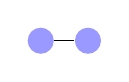
\begin{tikzpicture}
      [scale=.3,every node/.style={circle,fill=blue!40}]
      \node (n1) at (1,1) {};
      \node (n2) at (3,1) {};
      \draw (n1)--(n2);
    \end{tikzpicture}      
    & Edge, 1-star, 1-path, 2-clique
    & $m$ & \texttt{volume} \\

    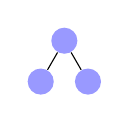
\begin{tikzpicture}
      [scale=.3,every node/.style={circle,fill=blue!40}]
      \node (n1) at (2,2.73) {};
      \node (n2) at (1,1) {};
      \node (n3) at (3,1) {};
      \draw (n1)--(n2);
      \draw (n1)--(n3);
    \end{tikzpicture}
    & Wedge, 2-star, 2-path
    & $s$ & \texttt{twostars} \\

    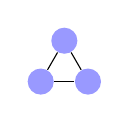
\begin{tikzpicture}
      [scale=.3,every node/.style={circle,fill=blue!40}]
      \node (n1) at (2,2.73) {};
      \node (n2) at (1,1) {};
      \node (n3) at (3,1) {};
      \draw (n1)--(n2);
      \draw (n1)--(n3);
      \draw (n2)--(n3); 
    \end{tikzpicture}
    & Triangle, 3-cycle, 3-clique 
    & $t$ & \texttt{triangles} \\

    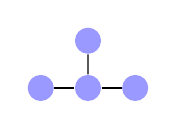
\begin{tikzpicture}
      [scale=.3,every node/.style={circle,fill=blue!40}]
      \node (n1) at (1,1) {};
      \node (n2) at (3,1) {};
      \node (n3) at (5,1) {};
      \node (n4) at (3,3) {};
      \draw (n1)--(n2);
      \draw (n2)--(n3);
      \draw (n2)--(n4);
    \end{tikzpicture}
    & Claw, 3-star 
    & $z$ & \texttt{threestars} \\

    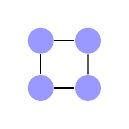
\begin{tikzpicture}
      [scale=.3,every node/.style={circle,fill=blue!40}]
      \node (n1) at (1,1) {};
      \node (n2) at (1,3) {};
      \node (n3) at (3,3) {};
      \node (n4) at (3,1) {};
      \draw (n1)--(n2);
      \draw (n2)--(n3);
      \draw (n3)--(n4);
      \draw (n4)--(n1); 
    \end{tikzpicture}
    & Square, 4-cycle 
    & $q$ & \texttt{squares} \\

    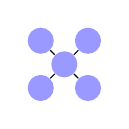
\begin{tikzpicture}
      [scale=.3,every node/.style={circle,fill=blue!40}]
      \node (n1) at (2,2) {};
      \node (n2) at (1,1) {};
      \node (n3) at (1,3) {};
      \node (n4) at (3,3) {};
      \node (n5) at (3,1) {};
      \draw (n1)--(n2);
      \draw (n1)--(n3);
      \draw (n1)--(n4);
      \draw (n1)--(n5);
    \end{tikzpicture}
    & Cross, 4-star 
    & $x$ & \texttt{fourstars} \\

    \midrule

    & $k$-Star
    & $S_k$ & \\

    & $k$-Path
    & $P_k$ & \\

    & $k$-Cycle
    & $C_k$ & \\

    & $k$-Clique 
    & $K_k$ & \\
    
    \bottomrule
  \end{tabular}
  }
\end{table}

A star is defined as a graph in which a central node is connected to all
other nodes, and no other edges are present. 
Specifically, a $k$-star is defined as a star in which the central node is
connected to $k$ other nodes.  Thus, a 2-star consists of a node
connected to two other nodes, or equivalently two incident edges, or a
path of length 2.  The specific name for 2-stars is \emph{wedges}.  The number of
wedges can be defined as 
\begin{align}
  \marginnote{\texttt{twostars}}
  s = \sum_{u \in V} {d(u) \choose 2} = \sum_{u \in V} \frac 1 2 d(u) (d(u) - 1),
\end{align}
where $d(u)$ is the degree of node $u$. 
Wedges have many different names:  2-stars, 2-paths,
hairpins \citep[e.g.][]{b853} and cherries.   

Three-stars are defined analogously to two-stars, and their count
denoted $z$.  Three-stars are also called \emph{claws} and
\emph{tripins} \citep[e.g.][]{b853}.   
\begin{align}
  \marginnote{\texttt{threestars}}
  z = \sum_{u \in V} {d(u) \choose 3} = \sum_{u \in V} \frac 1 6 d(u)
  (d(u) - 1) (d(u) - 2)
\end{align}

In the general case, the number of $k$-stars is defined as
\begin{align}
  S_k &= \sum_{u \in V} {d(u) \choose k}
\end{align}

The number of
triangles defined in the following way is independent of the orientation
of edges when the graph is directed.  Loops in the graph, as well as
edge multiplicities, are ignored.
\begin{align}
  \marginnote{\texttt{triangles}}
  t = | \{ \{u, v, w\} \mid u \leftrightarrow v \leftrightarrow w \leftrightarrow u \} | \;/\; 6
\end{align}

A square is a cycle of length four, and the number of squares in a graph
is denoted $q$.
\begin{align}
  \marginnote{\texttt{squares}}
  q = | \{ u, v, w, x \mid u \leftrightarrow v \leftrightarrow w \leftrightarrow x \leftrightarrow u \} | \;/\; 8
\end{align}
The factor 8 ensures that squares are counted regardless of their edge
labeling.  

Multiple edges are ignored in these count statistics, and edges in
patterns are not allowed to overlap. 

Triangles and squares are both cycles~-- which we can generalize to
$k$-cycles, sequences of $k$ distinct vertices that are cyclically
linked by edges.  We denote the number of $k$-cycles by $C_k$. 
For small $k$, we note the following equivalences: 
\begin{align*}
  C_1 &= 0 \\
  C_2 &= m \\
  C_3 &= t \\
  C_4 &= q
\end{align*}
for graphs without loops.  Cycles of length three and four have special
notation:  $C_3 = t$ and $C_4 = q$ and are called triangles and
squares. 

A cycle cannot the same node twice.  Due to this combinatorial
restriction, $C_k$ is quite complex to compute for large $k$.
Therefore, we may use \emph{tours} instead, defined as cyclical lists of
connected vertices in which we allow several vertices to overlap.  The
number of $k$-tours will be denoted $T_k$.  For computational
conveniance, we will define labeled tours, where two tours are not equal
when they are identical up to shifts or inversions.  
We note the following equalities: 
\begin{align}
  T_1 &= 0 \nonumber \\
  T_2 &= 2m \nonumber \\
  T_3 &= 6t \nonumber \\
  \marginnote{\texttt{tour4}}
  T_4 &= 8q + 4s + 2m 
\end{align}
Again, these are true when the graph is loopless.  The last equality
shows that trying to divide the tour count by $2k$ to count them up to
shifts and inversions is a bad idea, since it cannot be implemented by
dividing the present definition by $2k$. 

As mentioned before, counting cycles is a complex problem.  Counting
tours is however much easier.  The number of tours of length $k$ can be
expressed as the trace of a power of the graph's adjacency matrix, and
thus also as a moment of the adjacency matrix's spectrum when $k > 2$.  
\begin{align*}
  T_k &= \mathrm{Tr}(\mathbf A^k) = \sum_i \lambda_i[\mathbf A]^k
\end{align*}
This remains true when the graph includes loops.  

\subsection{Degree Distribution Statistics}
The distribution of degree values $d(u)$ over all nodes $u$ is often
taken to characterize a network.  Thus, a certain number of network
statistics are based solely on this distribution, regardless of overall
network structure.  
The simplest network statistics that depend only on the degree
distribution are the number of nodes $n$, the number of edges $m$ and
the average degree $d=2m/n$, as described previously.  More elaborative
statistics however reveal information about the detailed shape of the
degree distribution. 

The power law exponent is a number that characterizes the degrees of the
nodes in the network.  In many circumstances, networks are modeled to
follow a degree distribution power law, i.e., the number of nodes with
degree $n$ is taken to be proportional to the power $n^{-\gamma}$, for a
constant $\gamma$ larger than one \citep{b439}.  This constant $\gamma$
is called the power law exponent.  Given a network, its degree
distribution can be used to estimate a value $\gamma$.  There are
multiple ways of estimating $\gamma$, and thus a network does not have a
single definite value of it. In KONECT, we estimate $\gamma$ using the
robust method given in \citep[Eq.~5]{b408}
\begin{align}
  \marginnote{\texttt{power}} \gamma &= 1 + n \left( \sum_{u\in V} \ln
  \frac {d(u)} {d_{\min}} \right) ^{-1},
\end{align}
in which $d_{\min}$ is the minimal degree.

The Gini coefficient is a measure of inequality from economics,
typically applied to distributions of wealth or income.  In KONECT, we
apply it to the degree distribution, as described in
\citep{kunegis:power-law}.  The Gini coefficient can either be defined in
terms of the Lorenz curve, a type of plot that visualizes the inequality
of a distribution, or using the following expression.  Let $d_1 \leq d_2
\leq \dotsb \leq d_{n}$ be the sorted list of degrees in the
network. Then, the Gini coefficient is defined as
\begin{align}
  \marginnote{\texttt{gini}} G &= \frac {2 \sum_{i=1}^{n} i d_i} {n
    \sum_{i-1}^{n} d_i} - \frac {n+1} {n}.
\end{align}
The Gini coefficient takes values between zero and one, with zero
denoting total equality between degrees, and one denoting the dominance
of a single node.

The relative edge distribution entropy is a measure of the equality of
the degree distribution, and equals one when all degrees are equal, and
attains the limit value of zero when all edges attach to a single node
\citep{kunegis:power-law}.  It is defined as
\begin{align}
  \marginnote{\texttt{dentropyn}} H_{\mathrm{er}} &= \frac 1 {\ln n}
  \sum_{u \in V} - \frac{d(u)}{2m} \ln \frac{d(u)}{2m}.
\end{align}

Another statistic for \marginnote{\texttt{own}} measuring the inequality
in the degree distribution is associated with the Lorenz curve (see
Section~\ref{sec:plot:degree}), and is given by the intersection point
of the Lorenz curve with the antidiagonal given by $y = 1 - x$
\citep{kunegis:power-law}.  By construction, this point equals $(1-P, P)$
for some $0<P<1$, where the value $P$ corresponds exactly to the number
``25\%'' in the statement ``25\% of all users account for 75\% of all
friendship links on Facebook''.  By construction, we can expect $P$ to
be smaller when $G$ is large.

Another statistic, which has been called the ``hubiness'' is given by
the variance of the degree distribution \cite[e.g. by][]{b883,b884}.

Statistics such as the power law exponent $\gamma$, the Gini coefficient
$G$, the relative edge distribution entropy $H_{\mathrm{er}}$, as well
as the ratio $P$ all correlate with each other, as they measure the
inequality, skewness or ``hubiness'' of the degree distribution. 

The analysis of degrees can be generalized to pairs of nodes:  What is
the distribution of degrees for pairs of connected edges?  In some
networks, high-degree nodes are connected to other high-degree nodes,
while low-degree nodes are connected to low-degree nodes.  This property
is called assortativity \citep{b854}, or more precisely, the degree
assortativity.  Inversely, in a network with dissortativity,  
high-degree nodes are typically connected to low-degree and vice versa.
The amount of assortativity can be measured by the Pearson correlation
$\rho$ between the degree of connected nodes.  
\begin{align}
  \marginnote{\texttt{\small assortativity}} \rho &= \frac
  {\sum_{\{u,v\} \in E} (d(u) - d)(d(v) - d)}
  {\sum_{\{u,v\} \in E} (d(u) - d)^2}
\end{align}

The assortativity is
undefined whenever the Pearson correlation is undefined, for instance,
if all nodes have the same degree (i.e., when the graph is regular), and
when the graph does not contain any edges. 

\subsection{Clustering Statistics}
\label{sec:statistic:clustering}

The term \emph{clustering} refers to the observation that in almost all
networks, nodes tend to form small groups within which many edges are
present, and such that only few edges connected different clusters with
each other.  In a social network for instance, people form groups in
which almost every member known the other members.  Clustering thus
forms one of the primary characteristics of real-world networks, and
thus many statistics for measuring it have been defined.  The main
method for measuring clustering numerically is the clustering
coefficient, of which there exist several variants. As a general rule,
the clustering coefficient measures to what extent edges in a network
tend to form triangles. Since it is based on triangles, it can only be
applied to unipartite networks, because bipartite networks do not
contain triangles.

The number of triangles $t$ itself as defined in
Section~\ref{sec:count-statistics} is however not a statistic that can
be used to measure the clustering in a network, since it correlates with
the size and volume of the network.  Instead, the clustering
coefficients in all its variants can be understood as a count of
triangles, normalized in different ways in order to compare several
networks with it.

The local clustering coefficient $c(u)$ of a node $u$ is defined as the
probability that two randomly chosen (but distinct) neighbors of $u$ are
connected \citep{b228}.
\begin{align}
  c(u) &= \left\{ \begin{array}{ll} \frac { \{ v, w \in V \mid u \leftrightarrow v
      \leftrightarrow w \leftrightarrow u \} } { \{ v, w \in V \mid u \leftrightarrow v \neq w \leftrightarrow u \}
    } & \text{when } d(u) > 1 \\ 0 & \text{when } d(u) \leq 1
          \end{array} \right. 
\end{align}

The global clustering of a network can be computed in two ways.  The
first way defines it as the probability that two incident edges are
completed by a third edge to form a triangle \citep{b736}. This is also
called the transitivity ratio, or simply the transitivity.
\begin{align}
  \marginnote{\texttt{clusco}} c &= 
  \frac {|\{ u, v, w \in V \mid u \leftrightarrow v \leftrightarrow w \leftrightarrow u \}|} 
        {|\{ u, v, w \in V \mid u \leftrightarrow v \neq w \leftrightarrow u \}|} 
        = \frac {3t} s
\end{align}
This variant of the global clustering coefficient has values between
zero and one, with a value of one denoting that all possible triangles
are formed (i.e., the network consists of disconnected cliques), and
zero when it is triangle free.  Note that the clustering coefficient is
trivially zero for bipartite graphs.  This clustering coefficient is
however not defined when each node has degree zero or one, i.e., when
the graph is a disjoint union of edges and unconnected nodes.  This is
however not a problem in practice.

The second variant variant of the clustering coefficient uses the
average of the local clustering coefficients. This second variant was
historically the first to be defined.  In was defined in
1998 \citep{b228} and precedes the first variant by four years.
\begin{align}
  \marginnote{\texttt{clusco2}} c_2 &= \frac 1 {|V|} \sum_{u \in V} c(u)
\end{align}
This second variant of the global clustering coefficient is zero when a
graph is triangle-free, and one when the graph is a disjoint union of
cliques of size at least three.  This variant of the global clustering
coefficient is defined for all graphs, except for the empty graph, i.e.,
the graph with zero nodes.  A slightly different definition of the
second variant computes the average only over nodes with a degree of at
least two, as seen for instance in \citep{b845}.

Because of the arbitrary decision to define $c(u)$ as zero when the
degree of $c$ is zero or one, we recommend to use the first variant of
the clustering coefficient.  In the following, the extensions to the
clustering coefficient we present are all based on the first variant,
$c$.

For signed graphs, we may define the clustering coefficient to take into
account the sign of edges.  The signed clustering coefficient is based
on balance theory \citep{kunegis:slashdot-zoo}.  In a signed network,
edges can be positive or negative.  For instance in a signed social
network, positive edges represent friendship, while negative edges
represent enmity.  In such networks, balance theory stipulates than
triangles tend to be balanced, i.e., that three people are either all
friends, or two of them are friends with each other, and enemies with
the third.  On the other hand, a triangle with two positive and one
negative edge, or a triangle with three negative edges is unbalanced.
In other words, we can define the sign of a triangle as the product of
the three edge signs, which then leads to the stipulation that triangles
tend to have positive weight.  To extend the clustering coefficient to
signed networks, we thus distinguis between balanced and unbalanced
triangles, in a way that positive triangles contribute positively to the
signed clustering coefficient, and negative triangles contribute
negatively to it.  For a triangle $\{u,v,w\}$, let
$\sigma(u,v,w)=w(u,v)w(v,w)w(w,u)$ be the sign of the triangle, then the
following definition captures the idea:
\begin{align}
  c_{\mathrm s} &= \frac {\sum_{u,v,w\in V} \sigma(u,v,w)} {|\{ u, v, w
    \in V \mid u \leftrightarrow v \neq w \leftrightarrow u \}|}
\end{align}
Here, the sum is over all triangles $\{u,v,w\}$, but can also be taken
over all triples of vertices, since $w(u,v)=0$ when $\{u,v\}$ is not an
edge.

The signed clustering coefficient is bounded by the clustering
coefficient:
\begin{align}
  | c_{\mathrm s} | \leq c
\end{align}

The relative signed clustering coefficient can then be defined as
\begin{align}
  c_{\mathrm r} = \frac {c_{\mathrm s}} c = \frac {\sum_{u,v,w\in V}
    \sigma(u,v,w)} {|\{ u, v, w \in V \mid u \leftrightarrow v \leftrightarrow w \leftrightarrow u \}|}
\end{align}
which also equals the proportion of all triangles that are balanced,
minus the proportion of edges that are unbalanced.

\subsection{Distance Statistics}
\label{sec:distance-statistics}
The distance between two nodes in a network is defined as the number of
edges needed to reach one node from another, and serves as the basis for
a class of network statistics.

A path in a network is a sequence of incident edges, or equivalently, a
sequence of nodes $P = (u_0, u_2, \dotsc, u_k)$, such that $(u_i,
u_{i+1})\in E$ for all $i \in \{0, \dotsc, k-1\}$.  The number $k$ is
called the length of the path, and will also be denoted $l(P)$.  A
further restriction can be set on the visited nodes, definining that
each node can only be visited at most once. If the distinction is made,
the term \emph{path} is usually reserved for sequences of non-repeating
nodes, and general sequence of adjacent nodes are then called
\emph{walks}.  We will not make this distinction here.

Paths in networks can be used to model browsing behavior of people in
hyperlink networks, navigation in transport networks, and other types of
movement-like activities in a network.  When considering navigation and
browsing, an important problem is the search for shortest paths.  Since
the length of a path determines the number of steps needed to reach one
node from another, it can be used as a measure of distance between nodes
of a network.  The distance defined in this way may also be called the
shortest-path distance to distinguish it from other distance measures
between nodes of a network.
\begin{align}
  d(u, v) &= \left\{ \begin{array} {ll} \min_{P=(u, \dotsc, v)} l(P) &
    \text{when $u$ and $v$ are connected} \\ \infty & \text{when $u$ and
      $v$ are not connected}
  \end{array} \right. 
\end{align}
In the case that a network is not connected, the distance is defined as
infinite.  In practice, only the largest connected component of a
network may be used, making it unnecessary to deal with infinite values.
The distribution of all $|V|^2$ values $d(u,v)$ for all $u,v\in V$ is
called the distance distribution, and it too characterizes the network.

The eccentricity of a node can then be defined as the maximal distance
from that node to any other node, defining a measure of
\emph{non-centrality}:
\begin{align}
  \epsilon(u) &= \max_{v\in V} d(u,v)
\end{align}

The diameter $\delta$ of a graph equals the longest shortest path in the
network \citep{b779}.  It can be equivalently defined as the largest eccentricity of
all nodes.
\begin{align}
  \marginnote{\texttt{diam}} \delta &= \max_{u \in V} \epsilon(u) =
  \max_{u,v \in V} d(u,v)
\end{align}

Note that the diameter is undefined (or infinite) in unconnected
networks, and thus in numbers reported for actual networks in KONECT we
consider always the diameter of the network's largest connected
component.  Du to the high runtime complexity of computing the diameter,
it may be estimated by various methods, in which case it is noted noted
$\tilde \delta$.

A statistic related to the diameter is the radius, defined as the
smallest eccentricity
\begin{align}
  \marginnote{\texttt{radius}} r &= \min_{u \in V} \epsilon(u) = \min_{u
    \in V} \max_{v \in V} d(u,v)
\end{align}

The diameter is bounded from below by the radius, and from above by
twice the radius.  
\begin{align*}
  r \leq \delta \leq 2r
\end{align*}
The first inequality follows directly from the definitions of $r$ and
$\delta$ as the minimal and maximal eccentricity.  The second inequality
follows from the fact that between any two nodes, the path joining them
cannot be longer that the path joining them going through a node with
minimal eccentricity, which has length of at most $2r$. 

The radius and the diameter are not very expressive statistics: Adding
or removing an edge will, in many cases, not change their values.  Thus,
a better statistic that reflects the typical distances in a network in
given by the mean and average distance.

The mean path length $\delta_{\mathrm m}$ in a network is defined as as
the mean distance over all node pairs, including the distance between a
node and itself \citep{b779}:
\begin{align}
  \marginnote{\texttt{meandist}} \delta_{\mathrm m} &= \frac 1 {n^2}
  \sum_{u \in V} \sum_{v\in V} d(u,v)
\end{align}
The mean path length defined in this way is undefined when a graph is
disconnected.  Also, the average inverse distance has been used, or
equivalently, the inverse of the harmonic mean of distances \citep{b877}. 

\marginnote{\texttt{mediandist}}
Likewise, the median path length $\delta_{\mathrm M}$ is the median
length of shortest paths in the network.  In KONECT, both the median and
mean path lengths are computed taking into account node pairs of the
form $(u,u)$.

Both the mean and median path length can be called the
\emph{characteristic path length} of the network.

A related statistic is the 90-percentile effective diameter
$\delta_{0.9}$, which equals the number of edges needed on average to
reach 90\% of all other nodes.

\subsection{Algebraic Statistics}

Algebraic statistics are based on a network's characteristic matrices.
They are motivated by the broader field of spectral graph theory, which
characterizes graphs using the spectra of these matrices \citep{b285}.

In the following we will denote by $\lambda_k[\mathbf X]$ the
$k$\textsuperscript{th} dominant eigenvalue of the matrix $\mathbf X$.
For the adjacency matrix $\mathbf A$, the dominant eigenvalues are the
largest absolute ones; for the Laplacian $\mathbf L$ they are the
smallest ones.

Also, the matrix $\mathbf L$ will only be considered for the network's
largest connected component.

The spectral norm of a network equals the spectral norm (i.e., the
largest absolute eigenvalue) of the network's adjacency matrix
\begin{align}
  \marginnote{\texttt{snorm}} 
  \left\| \mathbf A \right\|_2
  &= 
  | \lambda_1[\mathbf A] | .
\end{align}
The spectral norm can be understood as an alternative measure of the
size of a network.

The algebraic connectivity equals the second smallest nonzero eigenvalue
of $\mathbf L$ \citep{b652}
\begin{align}
  \marginnote{\texttt{alcon}} a &= \lambda_2[\mathbf L].
\end{align}
The algebraic connectivity is zero when the network is disconnected~--
this is one reason why we restrict the matrix $\mathbf L$ to each
network's giant connected component.  The algebraic connectivity is
larger the better the network's largest connected component is
connected.

In signed and ratings networks, i.e., networks in which the weights of
node pairs can be negative, the smallest eigenvalue of $\mathbf L$ can
be larger than zero.  (In other networks, it is always zero.) The
algebraic conflict equals this smallest eigenvalue
\begin{align}
  \marginnote{\texttt{conflict}} \xi &= \lambda_1[\mathbf L].
\end{align}
The algebraic conflict measures the amount of conflict in the network,
i.e., the tendency of the network to contain cycles with an odd number
of negatively weighted edges.

\subsection{Bipartivity Statistics}
Some unipartite networks are almost bipartite.  Almost-bipartite
networks include networks of sexual contact \citep{b719} and ratings in
online dating sites \citep{b311,kunegis:split-complex-dating}.  Other,
more subtle cases, involve online social networks.  For instance, the
follower graph of the microblogging service Twitter is by construction
unipartite, but has been observed to reflect, to a large extent, the
usage of Twitter as a news service \citep{b545}. This is reflected in the
fact that it is possible to indentify two kinds of users: Those who
primarily get followed and those who primarily follow.  Thus, the
Twitter follower graph is almost bipartite.  Other social networks do
not necessarily have a near-bipartite structure, but the question might
be interesting to ask to what extent a network is bipartite.  To answer
this question, measures of bipartivity have been developed.

Instead of defining measures of bipartivity, we will instead consider
measures of non-bipartivity, as these can be defined in a way that they
equal zero when the graph is bipartite.  Given an (a priori) unipartite
graph, a measure of non-bipartivity characterizes the extent to which it
fails to be bipartite.  These measures are defined for all networks, but
are trivially zero for bipartite networks.  For non-bipartite networks,
they are larger than zero.

A first measure of bipartivity consists in counting the minimum number
of \emph{frustrated edges} \citep{b531}. Given a bipartition of vertices
$V=V_1\cup V_2$, a frustrated edge is an edge connecting two nodes in
$V_1$ or two nodes in $V_2$.  Let $f$ be the minimal number of
frustrated edges in any bipartition of $V$, or, put differently, the
minimum number of edges that have to be removed from the graph to make
it bipartite.  Then, a measure of non-bipartivity is given by
\begin{align}
  \marginnote{\texttt{frustration}} F &= \frac f {|E|}.
\end{align}
This statistic is always in the range $[0, 1/2]$.  It attains the value
zero if and only if $G$ is bipartite.

The minimal number of frustrated edges $f$ can be approximated by
algebraic graph theory.  First, we represent a bipartition $V = V_1 \cup
V_2$ by its characteristic vector $\mathbf x \in \mathbb R^{|V|}$
defined as
\begin{align*}
  \mathbf x_u &= \left\{ \begin{array}{ll} +1/2 & \text{when $u \in
      V_1$} \\ -1/2 & \text{when $u \in V_2$}
    \end{array} \right. 
\end{align*}
Note that the number of edges connecting the sets $V_1$ and $V_2$ is
then given by
\begin{align*}
\left\{ \{u,v\} \mid u \in V_1, v \in V_2 \right\} = \frac 12 \mathbf
x^{\mathrm T} \mathbf K[\bar G] \mathbf x &= \frac 12 \sum_{(u,v) \in E}
(\mathbf x_u + \mathbf x_v)^2,
\end{align*}
where $\mathbf K[\bar G] = \mathbf D[\bar G] + \mathbf A[\bar G]$ is the
signless Laplacian matrix of the underlying unweighted graph.  Thus, the
minimal number of frustrated edges $f$ is given by
\begin{align*}
  f &= \min_{\mathbf x \in \{\pm 1/2\}^{|V|}} \frac 12 \mathbf
  x^{\mathrm T} \mathbf K[\bar G] \mathbf x.
\end{align*}
By relaxing the condition $\mathbf x \in \{\pm 1/2\}^{|V|}$, we can
express $f$ in function of $\mathbf K[\bar G]$'s minimal eigenvalue,
using the fact that the norm of all vectors $\mathbf x \in \{\pm
1/2\}^{|V|}$ equals $\sqrt{|V|/4}$, and the property that the minimal
eigenvalue of a matrix equals its minimal Rayleigh quotient.
\begin{align*}
  \frac {2f} {|V|/4} &\approx \min_{\mathbf x \neq \mathbf 0} \frac
        {\mathbf x^{\mathrm T} \mathbf K[\bar G] \mathbf x} {\left\|
          \mathbf x \right\|^2} = \lambda_{\min}[\mathbf K[\bar G]]
\end{align*}
We can thus approximate the previous measure of non-bipartivity by
\begin{align}
  \marginnote{\texttt{anticonflict}} \tilde F &= \frac {|V|} {8 |E[\bar
      G]|} \lambda_{\min}[\mathbf K[\bar G]]
\end{align}
The eigenvalue $\lambda_{\min}[\mathbf K[\bar G]]$ can also be
interpreted as the algebraic conflict in $G$ interpreted as a signed
graph in which all edges have negative weight.

A further measure of bipartivity exploits the fact that the adjacency
matrix $\mathbf A$ of a bipartite graph has eigenvalues symmetric around
zero, i.e., all eigenvalues of a bipartite graph come in pairs $\pm
\lambda$. Thus, the ratio of the smallest and largest eigenvalues can be
used as a measure of non-bipartivity
\begin{align}
  \marginnote{\texttt{nonbip}} b_{\mathrm A} &= 1 - \left| \frac
             {\lambda_{\min}[\mathbf A[\bar G]]} {\lambda_{\max}[\mathbf
                 A[\bar G]]} \right|,
\end{align}
where $\lambda_{\min}$ and $\lambda_{\max}$ are the smallest and largest
eigenvalue of the given matrix, and $\bar G$ is the unweighted graph
underlying $G$.  Since the largest eigenvalue always has a larger
absolute value than the smallest eigenvalue (due to the
Perron--Frobenius theorem, and from the nonnegativity of $\mathbf A[\bar
  G]$), it follows that this measure of non-bipartivity is always in the
interval $[0,1)$, with zero denoting a bipartite network.  The value one
is excluded in non-empty loopless graphs.  This can be seen by
considering the trace of the graph's adjacency matrix, which equals the
sum of its diagonal values (and therefore equals the number of loops),
and at the same time equals the sum of eigenvalues of the adjacency
matrix. 

Another spectral measure of non-bipartivity is based on considering the
smallest eigenvalue of the matrix $\mathbf N[\bar G]$.  This eigenvalue
is $-1$ exactly when $G$ is bipartite.  Thus, this value minus one is a
measure of non-bipartivity. Equivalently, it equals two minus the
largest eigenvalue of the normalized Laplacian matrix $\mathbf Z$.
\begin{align}
  \marginnote{\texttt{nonbipn}} b_{\mathrm N} &= \lambda_{\min}[\mathbf
    N[\bar G]] + 1 = 2 - \lambda_{\max}[\mathbf Z[\bar G]]
\end{align}

\subsection{Signed Network Statistics}
In networks that allow negative edges such as signed networks and rating
networks, we may be interested in the proportion of edges that are
actually negative.  We call this the \emph{negativity} of the network. 
\begin{align}
  \marginnote{\texttt{negativity}}
  \zeta &= \frac { | \{ e \in E \mid w(e) < 0 \} | } {m}
\end{align}
The negativity is denoted $q$ in \citep{b868}. 

In directed signed networks, we can additionally compute the dyadic
conflict, i.e., the propostion of node pairs connected by two oppositely
oriented edges of different, compared to the total number of pairs of
nodes connected by two edges of opposite orientation. 
\begin{align}
  \marginnote{\texttt{dconflict}}
  \eta &= \frac 
       {|\{ u,v \mid u \rightleftarrows v, w(u,v) = - w(v,u) \}|} 
       {|\{ u, v \mid u \rightleftarrows v \}|}
\end{align}

Furthermore, the triadic conflict can be defined as the proportion of
triangles that are in conflict, i.e., that are unbalanced. 
\begin{align}
  \marginnote{\texttt{tconflict}}  
  T &= \frac 
  {\{ u, v, w \mid w(u, v) w(v, w) w(w, u) < 0\}}
  {\{ u, v, w \mid u \sim v \sim w \sim u \}}
\end{align}
This is also known as the triangle index.
It is also related to the relative signed clustering coefficient by
\begin{align*}
T &= 2 c_{\mathrm r} - 1.
\end{align*}

\subsection{Preferential Attachment Statistics}
The term \emph{preferential attachment} refers to the observation that
in networks that grow over time, the probability that an edge is added
to a node with $d$ neighbors is proportional to $d$.  This linear
relationship lies at the heart of Barabási and Albert's
\emph{scale-free} network model \citep{b439}, and has been used in a vast
number of subsequent work to model networks, online and offline. The
scale-free network model results in a distribution of degrees, i.e.,
number of neighbors of individual nodes, that follows a power law with
negative exponent. In other words, the number of nodes with degree $d$ is
proportional to $d^{-\gamma}$ in these networks, for a constant
$\gamma>1$.

In basic preferential attachment, the probability that an edge
attached to a vertex $u$ is propertional to its degree $d(u)$.  An
extension of this basic model uses a probability that is a power of the
degree, i.e., $d(u)^\beta$.  The exponent $\beta$ is a positive number,
and can be measured empirically from a dataset
\citep{kunegis:preferential-attachment}.  The value of $\beta$ then
determines the type of preferential attachment:
\begin{enumerate}
\item \textbf{Constant case $\beta=0$}.  
This case is equivalent to a constant probability of attachment, 
and thus this graph growth model results in networks in which each edge
is equally likely and independent from other edges.  This is the
Erdős--Rényi model of random graphs \citep{b569}. 

\item \textbf{Sublinear case $0 < \beta < 1$}. 
In this case, the preferential attachment function is sublinear.  This
model gives rise to a stretched exponential degree distribution
\citep{b764}, whose exact 
expression is complex and given in \citep[Eq. 94]{b773}. 

\item \textbf{Linear case $\beta=1$}.
This is the scale-free network model of Barabási and Albert
\citep{b439}, in which attachment is proportional to the degree. This gives a
power law degree distribution.  

\item \textbf{Superlinear case $\beta > 1$}.
In this case, a single node will acquire 100\% of all edges
asymptotically \citep{b765}. Networks with this behavior will however display
power law degree distributions in the pre-asymptotic regime
\citep{b769}. 
\end{enumerate}

The following minimization problem gives an estimate for the exponent
$\beta$ \citep{kunegis:preferential-attachment}.
\begin{align}
  \marginnote{\texttt{prefatt}}
  \min_{\alpha,\beta} \sum_{u\in V} \left( \alpha + \beta \ln[1 + d_1(u)]
  - \ln[\lambda + d_2(u)]  \right)^2
  \label{eq:min}
\end{align}
The resulting value of $\beta$ is the estimated preferential attachment
exponent. 

To measure the error of the fit, the root-mean-square
logarithmic error $\epsilon$ can be defined in the following way: 
\begin{align*}
    \epsilon &= \exp\left\{ \sqrt{ \frac 1 {|V|} \sum_{u \in V}
      \left(\alpha + \beta \ln[1 
        + d_1(u)] - \ln[\lambda + d_2(u)]\right)^2  }  \right\}
\end{align*}
This gives the average factor by which the actual new number of edges
differs from the predicted value, computed logarithmically. 
The value of $\epsilon$ is larger or equal to one by construction. 

\section{Node Features}
\label{sec:features}
A feature is a numerical characteristic of a node, such as the degree
and the eccentricity.  Features have multiple uses, such as to measure
the centrality or the influence of a node in a network. 

The degree is defined as the number 
\marginnote{\texttt{degree}}
of neighbors of a node.  In directed networks, we can distinguish the
indegree, the outdegree and the degree difference (indegree minus
outdegree, notes \texttt{degreediff}). 

Certain features are spectral, i.e., they are defined as the
eigenvectors of certain matrices.  For instance, the PageRank vector
\marginnote{\texttt{pagerank}} is defined as the dominant eigenvector of
the matrix $\mathbf G = (1-\alpha) \mathbf P + \alpha\mathbf J$. 

The local clustering coefficients give the clustering coefficient
distribution \marginnote{\texttt{cluscod}} \citep{b865}. 

\section{Graph Matrices and Decompositions}
\label{sec:matrix}
In order to analyse graphs, algebraic graph theory is a common
approach.  In algebraic graph theory, a graph with $n$ vertices is
represented by an $n\times n$ matrix called the adjacency matrix, from
which other matrices can be derived.  The defined matrices can then be
decomposed to reveal properties of the graph. 
In this section, we review characteristic graph matrices, their
decompositions, and their uses.  Since most decompositions are based on
a specific matrix, this section also serves as a survey of
characteristic graph matrices.  

Graph decompositions are implemented in the KONECT Toolbox by the
\texttt{konect\_decomposition()} function.  Each decomposition has a
name, which is given in the margin in the following. 

\subsection{Decompositions of Undirected Graphs}
These matrices and decompositions apply to undirected graphs.

In KONECT, these decompositions can be applied to directed graphs, in
which case edge directions are ignored. 

\subsubsection{Symmetric Adjacency Matrix ($\mathbf A$)}
The symmetric adjacency matrix $\mathbf A$ is the most basic graph
characteristic matrix.  It is a symmetric $n \times n$ matrix defined as
$\mathbf A_{uv}=1$ when the nodes $u$ and $v$ are connected, and
$\mathbf A_{uv}=0$ when $u$ and $v$ are not connected. 

The eigenvalue decomposition of the matrix $\mathbf A$ for undirected
graphs is widely used to analyse graphs: 
\begin{align}
  \marginnote{\texttt{sym}}
  \mathbf A &= \mathbf U \mathbf \Lambda \mathbf U^{\mathrm T}
\end{align}
$\mathbf \Lambda$ is an $n \times n$ real diagonal matrix containing the
eigenvalues of $\mathbf A$, i.e., $\mathbf \Lambda_{ii} =
\lambda_i[\mathbf A]$.  
$\mathbf U$ is an $n \times n$ orthogonal matrix having the
corresponding eigenvectors as columns. 

The largest absolute eigenvalue of $\mathbf A$ is the networks spectral norm,
i.e.,
\begin{align*}
  \max_i |\mathbf \Lambda_{ii}| &= \left\| \mathbf A \right\|_2.
\end{align*}

The sum of all eigenvalues $\lambda_i$ equal the trace of $\mathbf A$,
i.e., the sum of its diagonal elements.  The sum of the eigenvalues of
$\mathbf A$ thus equals the number of loops in the graphs. 
In particular, when a graph
has no loops, then the sum of the eigenvalues of its adjacency matrix is
zero.  

Higher moments the eigenvalues of $\mathbf A$ give the number of tours
in the graph.  Remember that a tour of length $k$ is defined as a
sequence of $k$ connected nodes, such that the first and the last node
are connected, such that two tours are considered as distinct when they
have a different starting node or orientation. 
The sum of $k$\textsuperscript{th} powers of the
eigenvalues of $\mathbf A$ then equals the number of $k$-tours $T_k$. 
We thus have in a loopless graph, that the traces of powers of $\mathbf
A$ are related to the number of edges $m$, the number of triangles $t$,
the number of squares $q$ and the number of wedges $s$ by:
\begin{align*}
  \mathrm{Tr}(\mathbf A) &= 0 \\
  \mathrm{Tr}(\mathbf A^2) &= 2m \\
  \mathrm{Tr}(\mathbf A^3) &= 6t \\
  \mathrm{Tr}(\mathbf A^4) &= 8q + 4s + 2m
\end{align*}
The traces of $\mathbf A$ can also be expressed as sums of powers
(moments) of the eigenvalues of $\mathbf A$:
\begin{align*}
  \mathrm{Tr}(\mathbf A^k) &= \sum_{i=1}^n \lambda_i^k
\end{align*}

The spectrum of $\mathbf A$ can also be characterized in terms of graph
bipartivity.  When the graph is bipartite, then all eigenvalues come in
pairs $\{\pm\lambda\}$, i.e., they are distributed around zero
symmetrically.  When the graph is not bipartite, then their distribution
is not symmetric.  It follows that when the graph is bipartite, the
smallest and largest eigenvalues have the same absolute value. 

\subsubsection{Laplacian Matrix ($\mathbf L$)}
The Laplacian matrix of an undirected graph is defined as
\begin{align*}
  \mathbf L &= \mathbf D - \mathbf A,
\end{align*}
i.e., the diagonal degree matrix from which we subtract the adjacency
matrix.  The Laplacian matrix is also called the Kirchhoff matrix. 

We consider the eigenvalue decomposition of the Laplacian:
\begin{align*}
  \marginnote{\texttt{lap}}
  \mathbf L &= \mathbf U \mathbf \Lambda \mathbf U^{\mathrm T}
\end{align*}
The Laplacian matrix of positive-semidefinite, i.e., all eigenvalues are
nonnegative.  
When the graph is unsigned, the smallest eigenvalue is zero and its
multiplicity equals the number of connected components in the graph. 

The second-smallest eigenvalue is called the algebraic connectivity of
the graph, and is denoted $a = \lambda_2[\mathbf L]$ \citep{b652}.  If the graph is
unconnected, that value is zero, i.e., an unconnected graph has an
algebraic connectivity of zero. 

When the graph is connected, the eigenvector corresponding to eigenvalue
zero is a constant vector, i.e., a vector with all entries equal. The
eigenvector corresponding the the second-smallest eigenvalue is called
the Fiedler vector, and can be used to cluster nodes in the
graph. Together with further eigenvectors, it can be used to draw
graphs \citep{kunegis:signed-kernels}. 

When the graph is signed, i.e., when the grpah admits edges with
negative weights, then the smallest eigenvalue of $\mathbf L$ is called
the algebraic conflict $\xi$. It is zero if and only if the graph is balanced,
i.e., when the nodes can be divided into two groups such that all
positive edges connect nodes within the same group, and all negative
edges connect nodes of different groups.  Equivalently, $\xi$ is larger
than zero if and only if each connected component contains at least one
cycle with an odd number of negative edges. 

\subsubsection{Normalized Adjacency Matrix ($\mathbf N$)}
The normalized adjacency matrix $\mathbf N$ of an undirected graph is
defined as 
\begin{align*}
  \mathbf N &= \mathbf D^{-1/2} \mathbf A \mathbf D^{-1/2},
\end{align*}
where we remind the reader that the diagonal matrix $\mathbf D$
contains the node degrees, i.e., $\mathbf D_{uu} = d(u)$. 
The matrix $\mathbf N$ is symmetric and its eigenvalue decomposition can
be considered:
\begin{align}
  \marginnote{\texttt{sym-n}}
  \mathbf N = \mathbf U \mathbf \Lambda \mathbf U^{\mathrm T}
\end{align}
The eigenvalues $\lambda_i$ of $\mathbf N$ can be used to characterize
the graph, in analogy with those of the nonnormalized adjacency
matrix.
The spectrum of $\mathbf N$ is also called the weighted spectral
distribution \citep{b864}.
All eigenvalues of $\mathbf N$ are contained in the range
$[-1,+1]$.  When the graph is unsigned, the largest eigenvalue is one.
In addition, the eigenvalue one has multiplicity one if the graph is
connected and unsigned.  It follows that for general unsigned graphs,
the multiplicity of the eigenvalue one equals the number of connected
components of the graph. 

Minus one is the smallest eigenvalue of $\mathbf N$ if and only iff the graph is
bipartite.  As with the nonnormalized adjacency matrix, the eigenvalues
of $\mathbf N$ are distributed symmetrically around zero if and only if
the graph is bipartite. 

When the graph is connected, 
the eigenvector corresponding to eigenvalue one has entries proportional
to the square root of node degrees, i.e.,
\begin{align*}
  \mathbf U_{u1} &= \sqrt{\frac{d(u)}{2m}}.
\end{align*}
Note that this equivalence only holds for undirected graphs.  For
directed graphs, there is no such equivalence. 

\subsubsection{Normalized Laplacian Matrix ($\mathbf Z$)}
The Laplacian matrix too, can be normalized.  It turns out that the
normalized Laplacian and the normalized adjacency matrix
are tighly related
to each other:  They share the same set of eigenvectors, and their
eigenvalues are reflections of each other.  

The normalized Laplacian matrix of an undirected graph is defined as 
\begin{align*}
  \mathbf Z &= \mathbf D^{-1/2} \mathbf L \mathbf D^{-1/2}.
\end{align*}
As opposed to $\mathbf A$, $\mathbf L$ and $\mathbf N$, there is no
standardized notation of the normalized Laplacian.  The notation
$\mathbf Z$ is specific to KONECT, and was chosen as the letter Z
resembles a turned letter N, and the matrices represented by those
letters share eigenvectors and have flipped eigenvalues. 

The normalized Laplacian is related to the normalized adjacency matrix
by 
\begin{align*}
  \mathbf Z &= \mathbf I - \mathbf N = \mathbf I - \mathbf D^{-1/2}
  \mathbf A \mathbf D^{-1/2}, 
\end{align*}
as can be derived directly from their definitions. 
It follows that $\mathbf Z$ and $\mathbf N$ have the same set of
eigenvectors, and that their eigenvalues are related by the
transformation $1 - \lambda$. Thus, the properties of $\mathbf Z$ can be
derived from those of $\mathbf N$. For instance, all eigenvalues of
$\mathbf Z$ are contained in the range $[0, 2]$, and the multiplicity of
the eigenvalue zero equals the number of connected components (when the
graph is unsigned). If the undirected graph is connected, the eigenvector of
eigenvalue zero contains entries proportional to the square root of the
node degrees. 

In KONECT, the decomposition of the normalized Laplacian is not
included, since it can be derived from that of the normalized adjacency
matrix. 

\subsubsection{Stochastic Adjacency Matrix ($\mathbf P$)}
The matrix
\begin{align*}
  \marginnote{\texttt{stoch1}}
  \mathbf P &= \mathbf D^{-1} \mathbf A
\end{align*}
is called the stochastic adjacency matrix.  This matrix is asymmetric,
even when the graph is undirected, except when the graph is regular,
i.e., when all degrees are the same.  
Thus, its eigenvalue decomposition
is not always defined, and in any case may not involve orthogonal
matrices. 

For directed graphs we may distinguish the right-stochastic (or
row-stochastic) matrix 
$\mathbf D^{-1} \mathbf A$ and the left-stochastic (or column-stochastic)
matrix $\mathbf A \mathbf D^{-1}$.  Note the subtle terminology:
$\mathbf D^{-1} \mathbf A$ is left-normalized but right-stochastic. 

This matrix is related to the normalized adjacency matrix $\mathbf N$ by
\begin{align*}
  \mathbf P &= \mathbf D^{-1/2} \mathbf N \mathbf D^{1/2}
\end{align*}
and therefore both matrices have the same set of eigenvalues.
Thus, the eigenvalues of $\mathbf P$ are all real, even though
$\mathbf P$ is asymmetric, and they are contained in the range $[-1,+1]$. 
Also, the relationship between $\mathbf P$ and $\mathbf N$ implies that that
eigenvectors of $\mathbf P$ are related to those of 
$\mathbf N$ by factors of the diagonal elements of $\mathbf D^{1/2}$,
i.e., the square roots of node degrees. 
Since $\mathbf P$ is asymmetric, its left eigenvectors differ from its
right eigenvectors.  When the graph is undirected, the left eigenvector
corresponding to the eigenvalue one has entries proportional to the
degree of nodes, 
while the right eigenvector corresponding to the eigenvalue one 
is the constant vector.  This is consistent with the fact that for a
random walk on an undirected graph, the stationary distribution of nodes
is proportional to the node degrees. 

The alternative matrix $\mathbf A \mathbf D^{-1}$ can also be
considered. \marginnote{\texttt{stoch2}} It is left-stochastic, and
can be derived by considering random walks that tranverse edges in a
backward direction. 

The matrix $\mathbf P$ is the state transition matrix of a random walk
on the graph, and thus its largest eigenvector is one if the graph is
(strongly) connected.  
The matrix $\mathbf P$ is also related to the PageRank matrix $\mathbf
G$ (``Google matrix''), which
equals 
\begin{align*}
  \mathbf G &= (1-\alpha) \mathbf P + \alpha\mathbf J
\end{align*}
where $0 < \alpha < 1$ is a damping factor (the teleportation
probability), and $\mathbf J$ is the matrix containing all ones.  The
left 
eigenvalues of the PageRank matrix give the PageRank values, and thus
we see that (ignoring the teleportation term), the PageRank of nodes in
an undirected network equals the degrees of the nodes. 

The matrix $\mathbf P$ is also related to random walks with restarts on
the graph, i.e., random walks that have a certain probability $0 <
\alpha < 1$
to return to an initial node at each step, instead of taking an edge at
random.  For any two nodes $u$ and $v$, the number
\begin{align}
  \left[\alpha  (\mathbf I - (1-\alpha) \mathbf P^{\mathrm T})^{-1}\right]_{uv}
\end{align}
gives the asymptotic probability that a random walk with restart starting at node $u$
stays at node $v$.  

The matrix $\mathbf P$ is further related to the mean first-passage time
(MFPT) on the network \citep{b880}.

\subsubsection{Stochastic Laplacian Matrix ($\mathbf S$)}
A further variant of the Laplacian exists, based on the stochastic
adjacency matrix:
\begin{align*}
  \mathbf S &= \mathbf I - \mathbf P = \mathbf I - \mathbf D^{-1}
  \mathbf A = \mathbf I - \mathbf D^{-1/2} \mathbf N \mathbf D^{1/2} =
  \mathbf D^{-1/2} \mathbf Z \mathbf D^{1/2}
\end{align*}
This matrix shares much properties with $\mathbf P$ and thus with
$\mathbf N$ and $\mathbf Z$.  The eigenvalues of $\mathbf S$ are
contained in the interval $[0, 2]$.  The eigenvalue zero has a
multiplicity equal to the number of connected components of the graph,
and when the graph is connected its corresponding right eigenvector is the
constant vector, while its corresponding left eigenvector is
proportional to the node degrees.  For connected graphs, the largest
eigenvalue of $\mathbf S$ is two if and only if the graph is bipartite.
In the general case, the eigenvalue two has a multiplicity equal to the
number of connected components that are bipartite. 

\subsubsection{Signless Laplacian ($\mathbf K$)}
The signless Laplacian of a graph is defined as the Laplacian of the
corresponding graph in which all edges are interpreted as negative.  It
thus equals
\begin{align}
  \marginnote{\texttt{lapq}}
  \mathbf K &= \mathbf D + \mathbf A
\end{align}
This matrix is positive-semidefinite, and its smallest eigenvalue is
zero if and only if the graph is bipartite.  Thus, $\mathbf K$ is used
in measures of bipartivity. 

\subsubsection{Alternative Signed Laplacian}
The Laplacian matrix $\mathbf L = \mathbf D - \mathbf A$ as defined
earlier is based on the the degree matrix $\mathbf D$, whose diagonal
elements equal the sum of absolute weights of all edges incident to each
node.  
Taking the absolute value in that definition is justified for
many applications related to signed graphs, and results in a positive-semidefinite matrix, whose
smallest eigenvalue is zero if and only if there is at least one
balanced component in the signed network.  Alternatively, using the sum
of edge weights instead results in a different matrix, which may have
negative eigenvalues.  This matrix appears in certain contexts; see
e.g.\ the examples given by \cite{b875}. 

\subsection{Decompositions of Directed Graphs}
In directed graphs, the adjacency matrix $\mathbf A$ is itself
asymmetric, and there is no special half-adjacency matrix.  Since the
adjacency matrix is symmetric, decompositions are more complex.  For
instance, $\mathbf A$ is not normal in the general case, and therefore
there is no simply defined eigenvalue decomposition anymore. 

\subsubsection{Singular Value Decomposition}
The singular value decomposition is defined for any matrix, including
those that are not symmetric, and even those that are not quadratic.
Thus, it can be applied to the adjacency matrix of directed graphs. 
\begin{align}
  \marginnote{\texttt{svd}}
  \mathbf A &= \mathbf U \mathbf \Sigma \mathbf V^{\mathrm T}
\end{align}
The matrices $\mathbf U$ and $\mathbf V$ are each orthogonal, but they
are not equal.  They contain the left and right singular vectors are
columns.  The matrix $\mathbf \Sigma$ is diagonal, and contains the
singular values, which are all nonnegative. 

\subsubsection{Normalized Adjacency Matrix}
The adjacency matrix can be normalized for directed network, in the same
way as for undirected networks.
\begin{align}
  \mathbf N &= \mathbf D_{\mathrm O}^{-1/2} \mathbf A \mathbf D_{\mathrm I}^{-1/2}
\end{align}
Here, $\mathbf D_{\mathrm O}^{-1/2}$ and $\mathbf D_{\mathbf I}^{-1/2}$
are the diagonal matrices of out- and indegrees. 

The normalized adjacency matrix $\mathbf N$ can be used in the singular
value decomposition, too:
\begin{align}
  \marginnote{\texttt{svd-n}}
  \mathbf N &= \mathbf U \mathbf \Sigma \mathbf V^{\mathrm T}
\end{align}

\subsubsection{Eigenvectors}
While the eigenvalue decomposition is not defined in the general case
for an asymmetric matrix $\mathbf A$, its eigenvectors and eigenvalues
are well-defined, if we distinguish between left and right
eigenvectors.

\marginnote{\texttt{diag}}
Thus, we define the method \texttt{diag}, which is a decomposition in
the KONECT sense, but not in the strict mathematical sense. 
$\mathbf U$ and $\mathbf V$ are then defined as the matrices containing
the left and right eigenvectors of $\mathbf A$, and $\mathbf \Lambda$ is
the diagonal matrix of corresponding eigenvalues. 

Note that while left and right eigenvectors differ, their eigenvalues
are identical. 

\subsubsection{Skew Adjacency Matrix ($\mathbf Y$)}
While an asymmetric matrix $\mathbf A$ may be transformed to $\mathbf A
+ \mathbf A^{\mathrm T}$ to give a symmetric matrix, we can also use
$\mathbf Y = \mathbf A - \mathbf A^{\mathrm T}$ to get a skew-symmetric matrix.  A
skew symmetric matrix $\mathbf X$ is a matrix such that $\mathbf X =
-\mathbf X^{\mathrm T}$.

Skew symmetric matrices have well-defined eigenvalue decompositions,
which are however complex, as both the eigenvectors and eigenvalues will
be complex numbers.  The eigenvectors and eigenvalues however follow a
specific pattern, that we can exploit to represent such a decomposition
using only real numbers:
\begin{align}
  \mathbf Y &= \mathbf A - \mathbf A^{\mathrm T} = \mathbf Q \mathbf R \mathbf Q^{\mathrm T}
\end{align}
such that
\begin{align}
  \mathbf Q &= \frac 1 {\sqrt{2}} \left[
    \begin{array}{cc}
      \mathbf U + i \mathbf V \\
      \mathbf U - i \mathbf V 
    \end{array}
    \right] \\
  \mathbf R &= \left[ \begin{array}{cc}
      i \mathbf D & \mathbf 0 \\
      \mathbf 0 & -i \mathbf D
    \end{array} \right]
\end{align}
where $\mathbf U$, $\mathbf V$ and $\mathbf D$ are real matrices.  In
fact, this decomposition can be equivalently written as
\begin{align}
  \marginnote{\texttt{skew}}
  \mathbf Y = \mathbf A - \mathbf A^{\mathrm T} &=
  \mathbf U \mathbf D \mathbf V^{\mathrm T} - \mathbf V \mathbf D \mathbf U^{\mathrm T}.
\end{align}
This decomposition is equivalent to that given by 
\cite{b869}.  It shows that the skew-symmetric matrix $\mathbf Y$ has
eigenvalues that are purely imaginary, come  
in pairs $\{\pm i \lambda\}$ that are the negative of each other (or
equivalently, the complex conjugate), and their corresponding
eigenvectors are also complex conjugates of each other.

Note also that the number of columns of both $\mathbf U$ and $\mathbf V$
is at most $\lfloor n \rfloor$, and thus, if $n$ is odd, the
skew-symmetric matrix $\mathbf Y$ has the
eigenvalue zero, which is the complex conjugate of itself.  Also, the
expression $\mathbf U \mathbf D \mathbf V^{\mathrm T}$ is \emph{not} the
singular value decomposition of $\mathbf A$, even if the form of the
decomposition is the same. 

\subsubsection{Hermitian Adjacency Matrix ($\mathbf H$)}
In certain contexts, for instance when constructing the Hamiltonian of a
system, it is necessary to specify Hermitian matrices, i.e.,
diagonalizable matrices that have only real eigenvalues.  To take into
account all connectivity information of a directed graph in a
directed graph, the symmetric and skew-symmetric adjacency matrices can
be combined in the following way:
\begin{align}
  \marginnote{\texttt{herm}}
  \mathbf H &= \frac 1 {\sqrt 2} \left[
  \mathbf A + \mathbf A^{\mathrm T} + i(\mathbf A - \mathbf A^{\mathrm T})
  \right]. 
\end{align}
The matrix $\mathbf H$ is Hermitian, i.e., it equals the complex
conjugate of its transpose, $\mathbf H = \mathbf {\bar H}^{\mathrm T} =
\mathbf H^{\dagger}$.
Furthermore, the Hermitian adjacency matrix can be defined by
\begin{align}
  \mathbf H_{uv} &= \exp\left\{i \frac \pi 4 \mathbf Y_{uv}\right\},
\end{align}
which additionally justifies the factor $1/\sqrt 2$ in the initial
definition of $\mathbf H$, as $e^{i \frac \pi 4} = 1/\sqrt 2 + i/\sqrt
2$.  Using this form, the Hermitian adjacency matrix can be generalized
to the matrix $\mathbf H_\alpha$ where $0 \leq \alpha \leq \pi/2$ is a
real parameter, giving 
\begin{align}
  [\mathbf H_{\alpha}]_{uv} &= \exp\left\{i \alpha \mathbf Y_{uv} \right\},  
\end{align}
from which the following special cases can be recovered:
\begin{align}
  \mathbf H_0 &= \mathbf A + \mathbf A^{\mathrm T}, \\
  \mathbf H_{\pi/4} &= \mathbf H, \\
  \mathbf H_{\pi/2} &= \mathbf Y.
\end{align}
These matrices appear in the modeling of quantum walks, as used for
instance by \cite{toedtli:ctqw}.  

\section{Network Plots}
\label{sec:plots}
Plots are drawn to visualize a certain aspect of a dataset. These plots
can be used to compare several network visually, or to illustrate the
definition of a certain numerical statistic.

As a running example, we show the plots for the Wikipedia elections
network
(\href{http://konect.uni-koblenz.de/networks/elec}{\textsf{EL}}).  Plots
for all networks (in which computation was feasible) are shown on the
KONECT
website\footnote{\href{http://konect.uni-koblenz.de/plots/}{konect.uni-koblenz.de/plots}}. The
KONECT Toolbox contains Matlab code for generating these plot types.

\subsection{Layout}
Layout plots show the nodes and edges of a graph in a way that makes
features if the graph visible.  Usually, this only makes sense for small
graphs.\footnote{See
  \href{https://networkscience.wordpress.com/2016/06/22/no-hairball-the-graph-drawing-experiment/}{networkscience.wordpress.com/2016/06/22/no-hairball-the-graph-drawing-experiment}
  for an explanation.}
In KONECT, we use the algorithm of \cite{b870}.  An
example is shown in Figure~\ref{fig:fruchterman-reingold}.

\begin{figure}
  \centering
  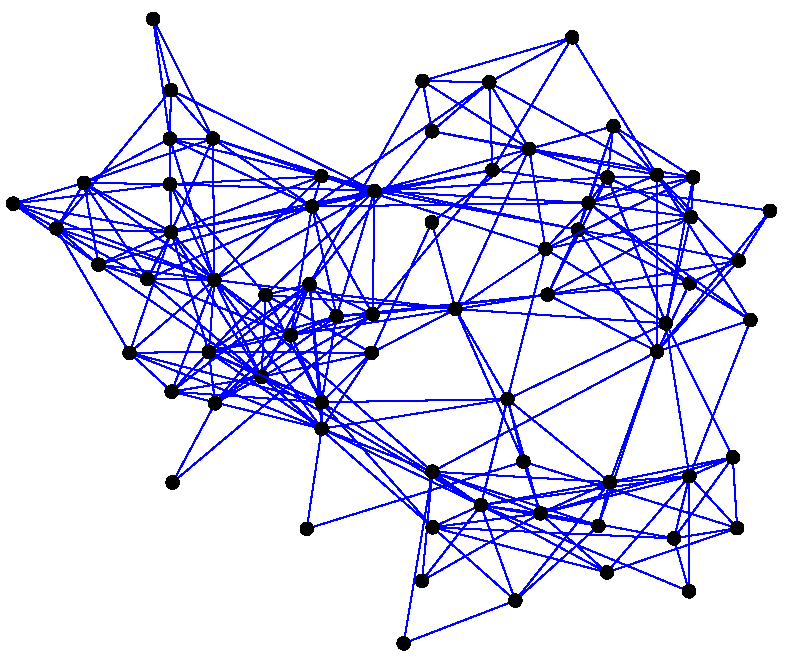
\includegraphics[width=\wPlot]{plot/layout.a.moreno_highschool}
  \caption{
    \label{fig:fruchterman-reingold}
    The layout of the highschool social network given by \cite{konect:coleman}
    (\href{http://konect.uni-koblenz.de/networks/moreno_highschool}{\textsf{MH}}),
    generated using the algorithm of \cite{b870}.  This network has 70 vertices,
    and for such small networks, drawing a graph leads to sensible
    plot.  For large graphs, graph drawing usually lead to
    ``hairball''-like plots and are thus less useful.
  }
\end{figure}

\subsection{Temporal Distribution}
The temporal distributions shows the distribution of edge creation
times.  It is only defined for networks with known edge creation times.
The X axis is the time, and the Y axis is the number of edges added
during each time interval.

\begin{figure}
  \centering 
  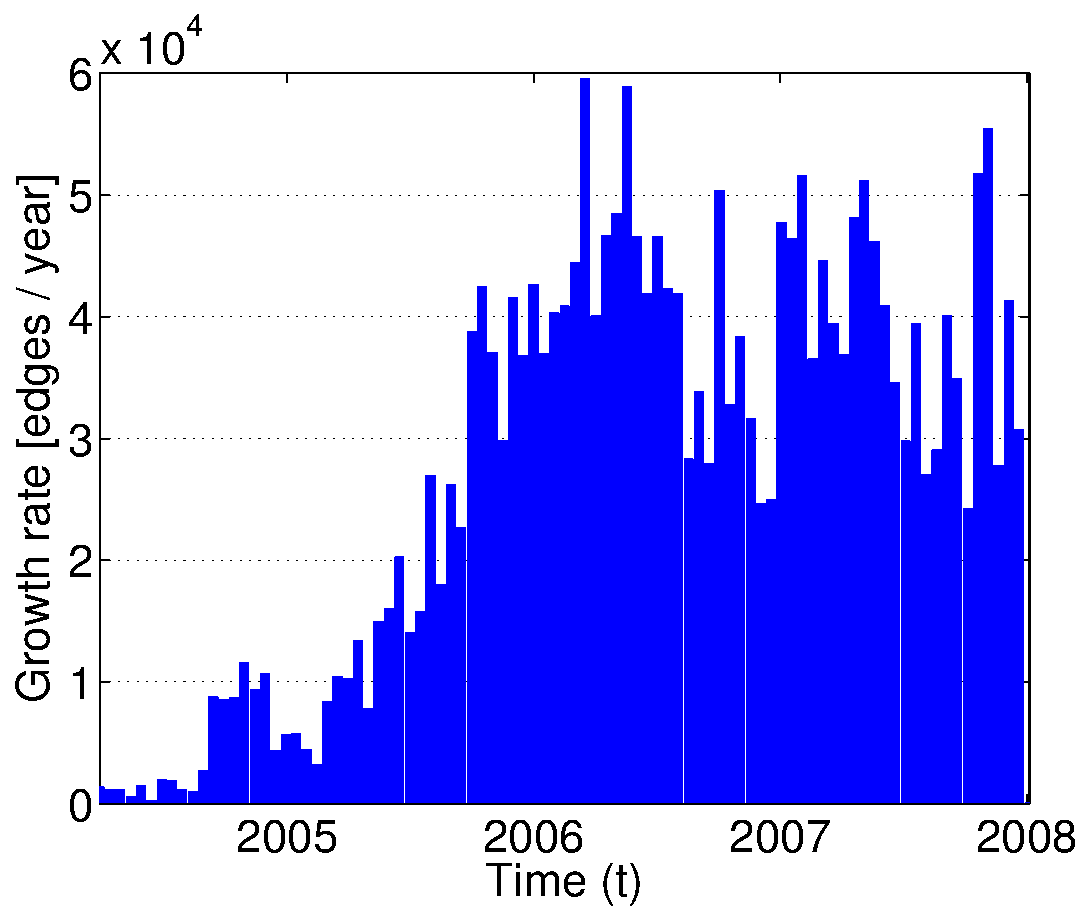
\includegraphics[width=\wPlot]{plot/time_histogram.elec}
  \caption{ 
    The temporal distribution of edges for the Wikipedia
    elections network.  
  }
\end{figure}

\subsection{Edge Weight and Multiplicity Distribution}
The edge weight and multiplicity distribution plots show the
distribution of edge weights and of edge multiplicities, respectively.
They are not generated for unweighted networks.  The X axis shows values
of the edge weights or multiplicities, and the Y axis shows frequencies.
Edge multiplicity distributions are plotted on doubly logarithmic
scales.

\begin{figure}
  \centering 
  \subfigure[Edge weight distribution]{
    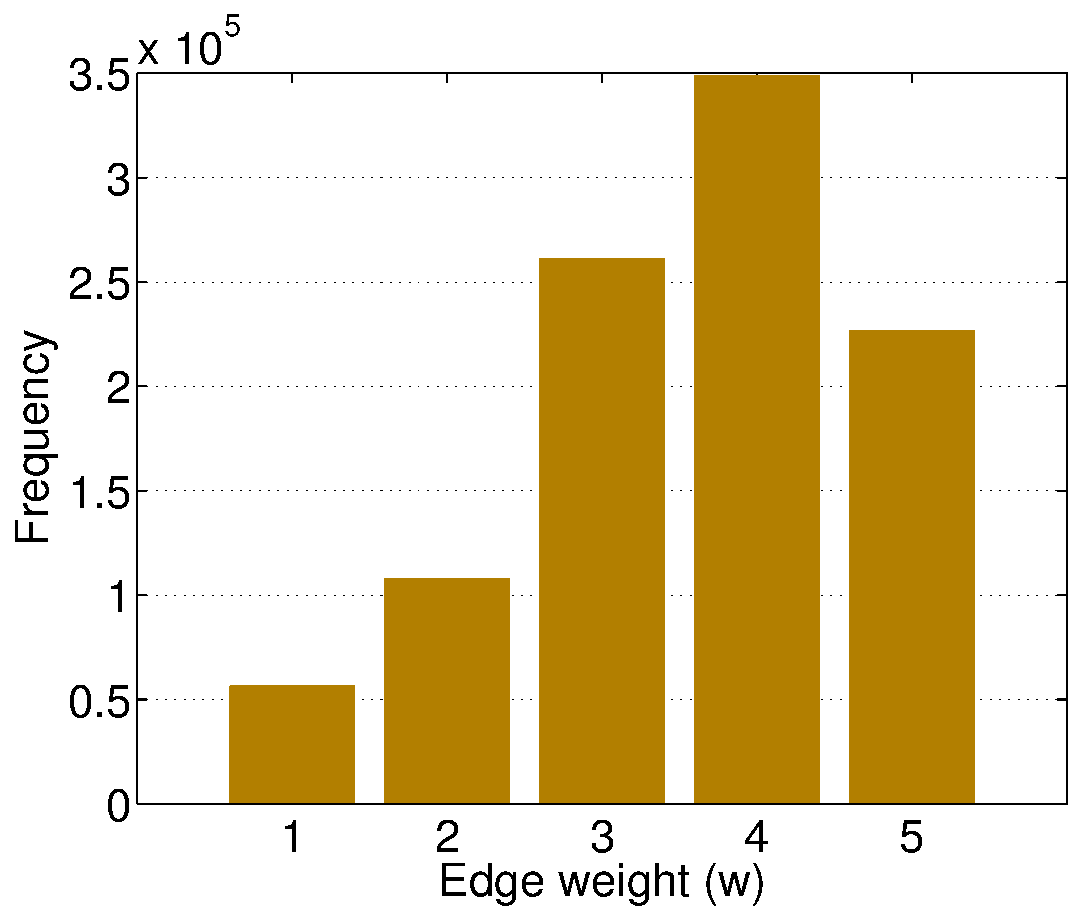
\includegraphics[width=\wPlot]{plot/weights.b.movielens-1m}}
  \subfigure[Edge multiplicity distribution]{
    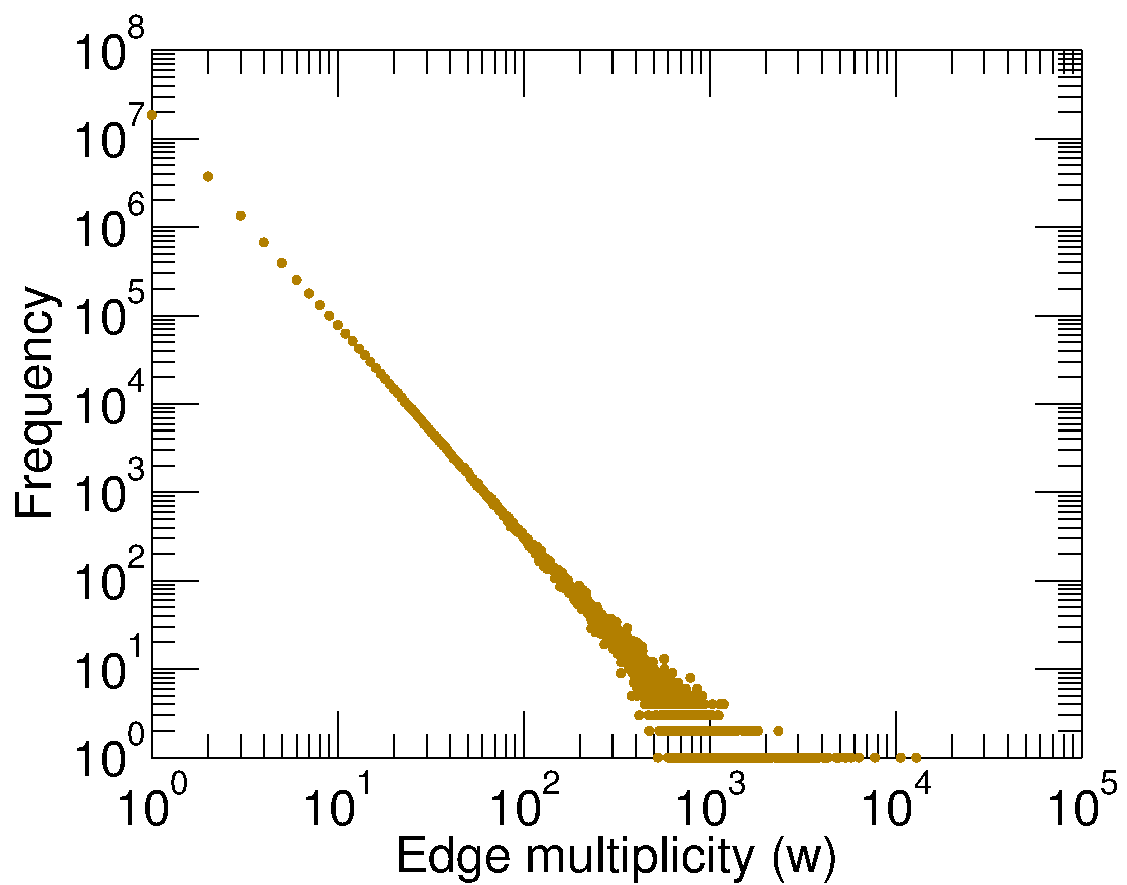
\includegraphics[width=\wPlot]{plot/weights.c.edit-dewiki}}
  \caption{ 
    \label{fig:weight}
    The distribution of (a)~edge weights for the MovieLens
    rating network
    (\href{http://konect.uni-koblenz.de/networks/movielens-1m}{\textsf{M2}})
    and (b)~edge multiplicities for the German Wikipedia edit network
    (\href{http://konect.uni-koblenz.de/networks/edit-dewiki}{\textsf{de}}).
  }
\end{figure}

\subsection{Degree Distribution} 
\label{sec:plot:degree}
The distribution of degree values $d(u)$ over all vertices $u$
characterizes the network as a whole, and is often used to visualize a
network. In particular, a power law is often assumed, stating that the
number of nodes with $n$ neighbors is proportional to $n^{-\gamma}$, for
a constant $\gamma$ \citep{b439}. This assumption can be inspected
visually by plotting the degree distribution on a doubly logarithmic
scale, on which a power law renders as a straight line.  KONECT supports
two different plots: The degree distribution, and the cumulative degree
distribution. The degree distribution shows the number of nodes with
degree $n$, in function of $n$.  The cumulative degree distribution
shows the probability that the degree of a node picked at random is
larger than $n$, in function of $n$. Both plots use a doubly logarithmic
scale.

Another visualization of the degree distribution supported by KONECT is
in the form of the Lorenz curve, a type of plot to measure inequality
originally used in economics (not shown).

\begin{figure}
  \centering 
  \subfigure[Degree distribution]{
    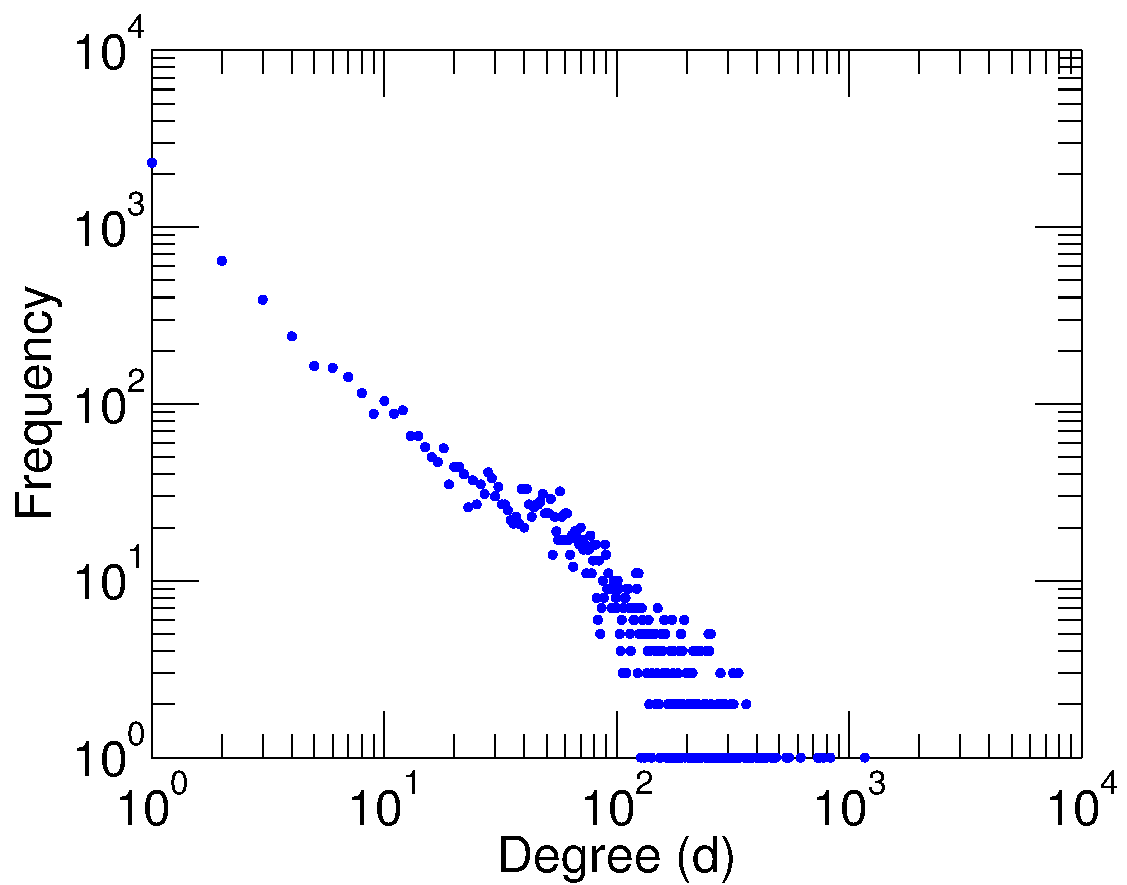
\includegraphics[width=\wPlot]{plot/degree.a.elec}}
  \subfigure[Cumulative degree distribution]{
    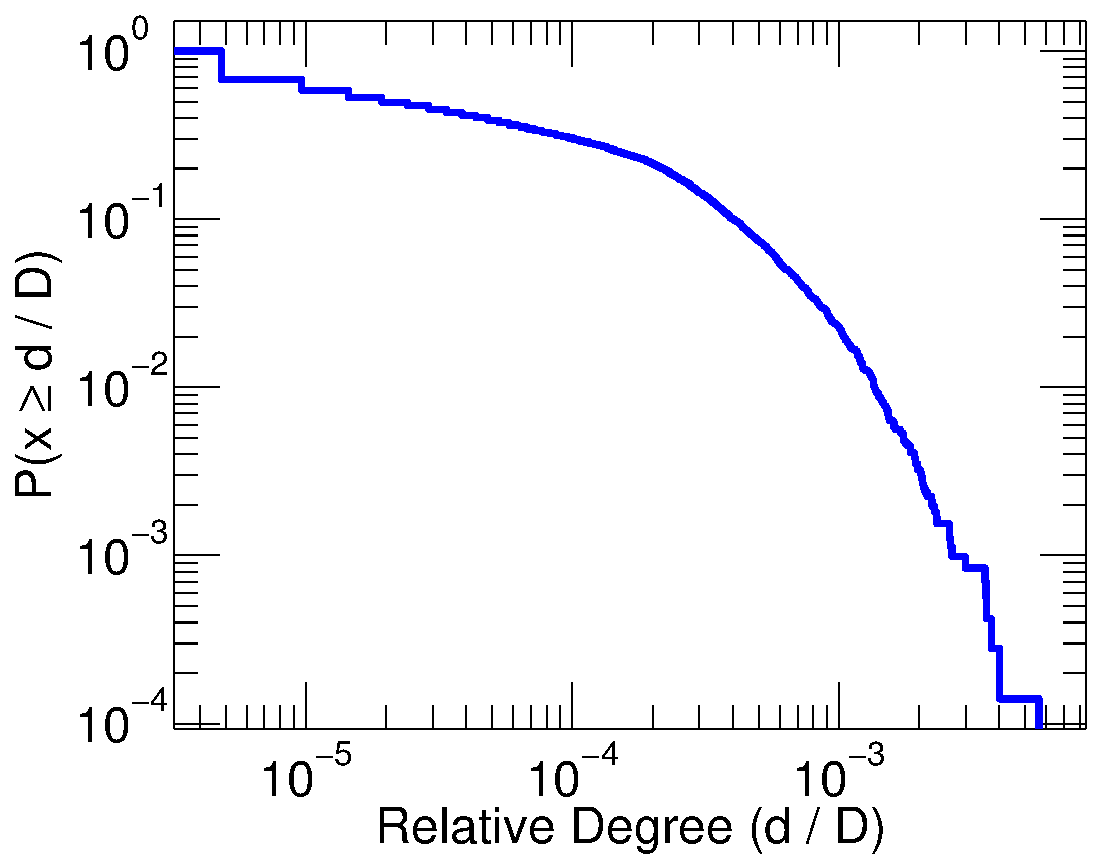
\includegraphics[width=\wPlot]{plot/bidd.a.elec}}
  \caption{ 
    \label{fig:degree}
    The degree distribution and cumulative degree distribution
    for the Wikipedia election network
    (\href{http://konect.uni-koblenz.de/networks/elec}{\textsf{EL}}).
  }
\end{figure}

The Lorenz curve is a tool originally from economics that visualizes
statements of the form ``X\% of nodes with smallest degree account for
Y\% of edges''.  The set of values $(X,Y)$ thus defined is the Lorenz
curve. In a network the Lorenz curve is a straight diagonal line when
all nodes have the same degree, and curved
otherwise \citep{kunegis:power-law}.  The area between the Lorenz curve
and the diagonal is half the Gini coefficient (see above).

\begin{figure}
  \centering 
  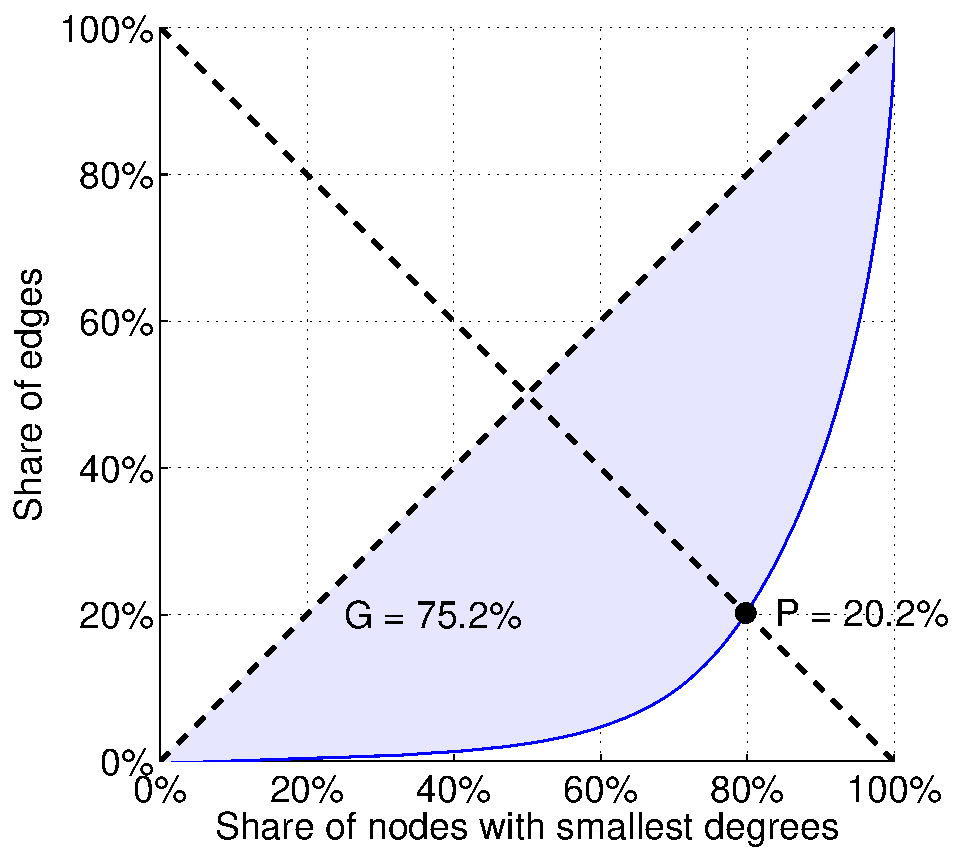
\includegraphics[width=\wPlot]{plot/lorenz.a.elec}
  \caption{ 
    The Lorenz curve for the Wikipedia election network
    (\href{http://konect.uni-koblenz.de/networks/elec}{\textsf{EL}}).
    \label{fig:lorenz}
  }
\end{figure}

\subsection{Out/indegree Comparison}
The out/indegree comparison plots show the joint distribution of
outdegrees and indegrees of all nodes of directed graphs.  The plot
shows, for one directed network, each node as a point, which the
outdegree on the X axis and the indegree on the Y axis.  

An example is shown in Figure~\ref{fig:outin} for the Wikipedia
elections network. 

\begin{figure}
  \centering
  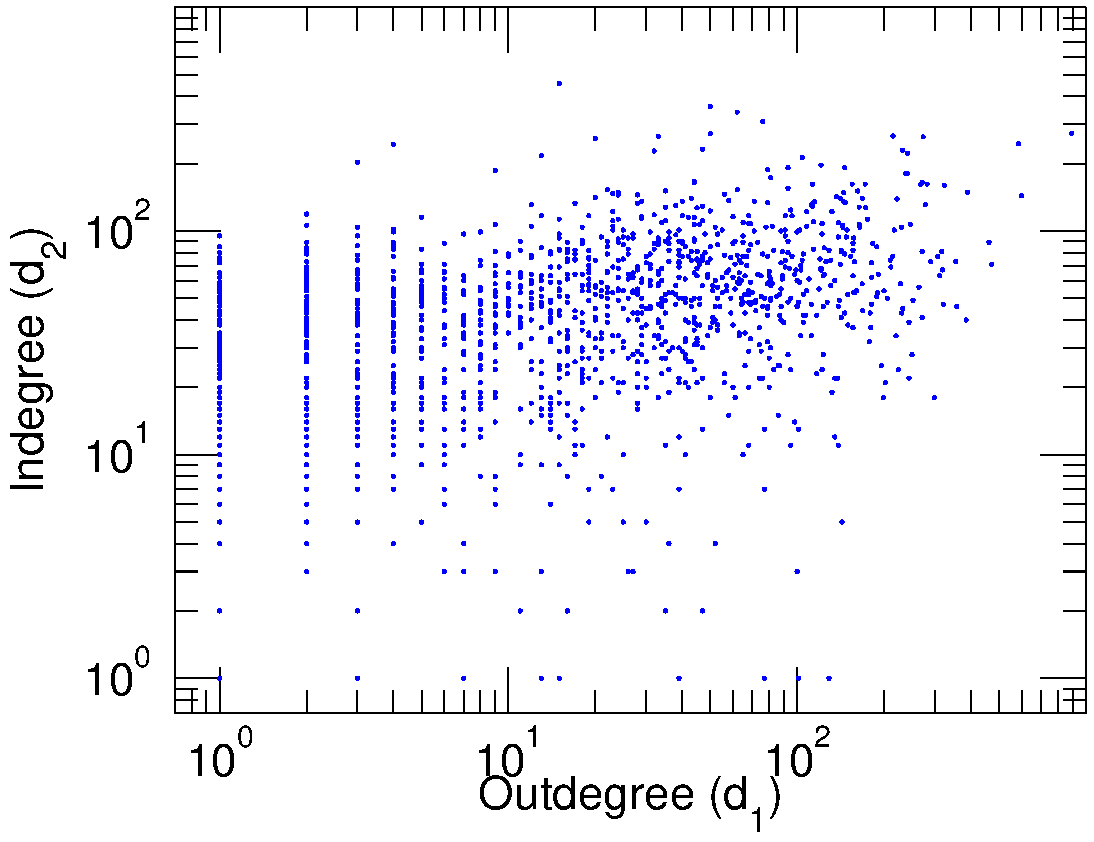
\includegraphics[width=\wPlot]{plot/outin.b.elec}
  \caption{
    \label{fig:outin}
    The out/indegree comparison plot of the Wikipedia election network 
    (\href{http://konect.uni-koblenz.de/networks/elec}{\textsf{EL}}).
  }
\end{figure}

\subsection{Assortativity Plot}
In some networks, nodes with high degree are more often connected with
other nodes of high degree, while nodes of low degree are more often
connected with other nodes of low degree.  This property is called
assortativity, i.e., such networks are said to be assortativity.  On the
other hand, some networks, are dissortative, i.e., in them nodes of high
degree are more often connected to nodes of low degree and vice versa.
In addition to the assortativity $\rho$ defined as the Pearson
correlation coefficient between the degrees of connected nodes, the
assortativity or dissortativity of networks may be analyse by plotting
all nodes of a network by their degree and the average degree of their
neighbors.  Thus, the assortativity plot of a network shows all nodes of
a network with the degree on the X axis, and the average degree of their
neighbors on the Y axis. 

An example of the assortativity plot is shown for the Wikipedia
elections network in Figure~\ref{fig:assortativity}. 

\begin{figure}
  \centering
  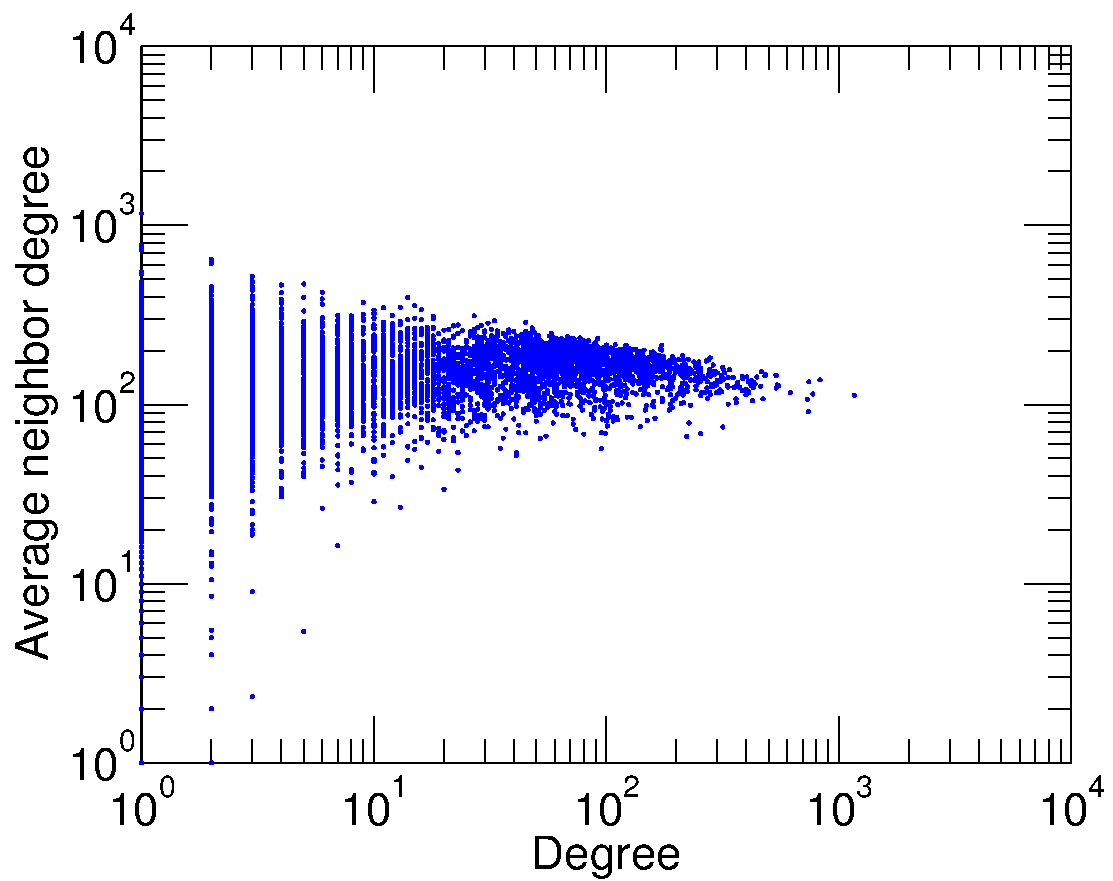
\includegraphics[width=\wPlot]{plot/assortativity.a.elec}
  \caption{
    The assortativity plot of the Wikipedia election network 
    (\href{http://konect.uni-koblenz.de/networks/elec}{\textsf{EL}}).
    \label{fig:assortativity}
  }
\end{figure}

\subsection{Clustering Coefficient Distribution}
In Section~\ref{sec:statistic:clustering}, we defined the clustering
coefficient of a node in a graph as the propotion of that node's
neighbors that are connected, and proceeded to define the clustering
coefficient as the corresponding measure applied to the whole network.
In some case however, we may be interested in the distribution of the
clustering coefficient over the nodes in the network.  For instance, a
network could have some very clustered parts, and some less clustered
parts, while another network could have many nodes with a similar,
average clustering coefficient.  Thus, we may want to consider the
distribution of clustering coefficient.  This distribution can be
plotted as a cumulated plot.

\begin{figure}
  \centering
  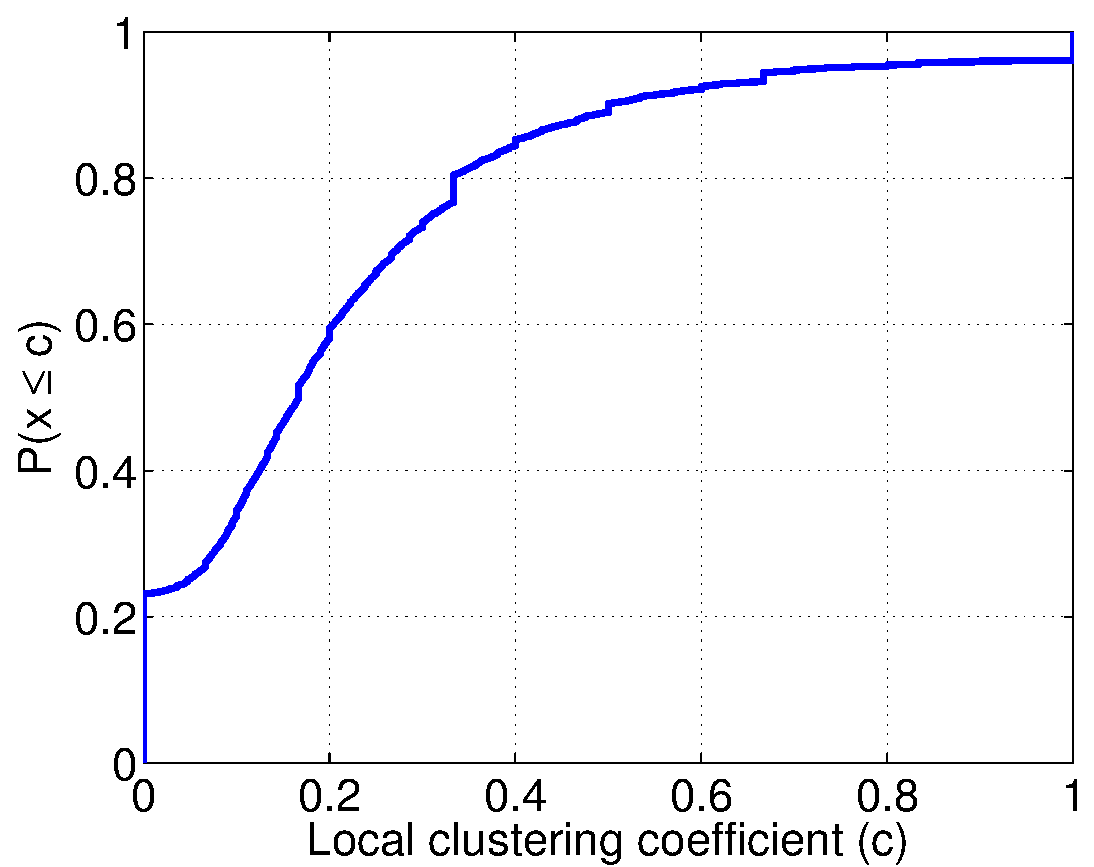
\includegraphics[width=\wPlot]{plot/cluscod.a.facebook-wosn-links}
  \caption{ The clustering coefficient distribution for Facebook link
    network~(\href{http://konect.uni-koblenz.de/networks/facebook-wosn-links}{\textsf{Ol}}).
  }
\end{figure}

\subsection{Spectral Plot}
The eigenvalues of a network's characteristic matrices $\mathbf A$,
$\mathbf N$ and $\mathbf L$ are often used to characterize the network
as a whole.  KONECT supports computing and visualizing the spectrum
(i.e., the set of eigenvalues) of a network in multiple ways.  Two types
of plots are supported: Those showing the top-$k$ eigenvalues computed
exactly, and those showing the overall distribution of eigenvalues,
computed approximately. The eigenvalues of $\mathbf A$ are positive and
negative reals, the eigenvalues of $\mathbf N$ are in the range
$[-1,+1]$, and the eigenvalues of $\mathbf L$ are all nonnegative.  For
$\mathbf A$ and $\mathbf N$, the largest absolute eigenvalues are used,
while for $\mathbf L$ the smallest eigenvalues are used.  The number of
eigenvalue shown $k$ depends on the network, and is chosen by KONECT
such as to result in reasonable runtimes for the decomposition
algorithms.

\begin{figure}
  \centering \subfigure[Top-$k$ eigenvalues of $\mathbf A$]{
    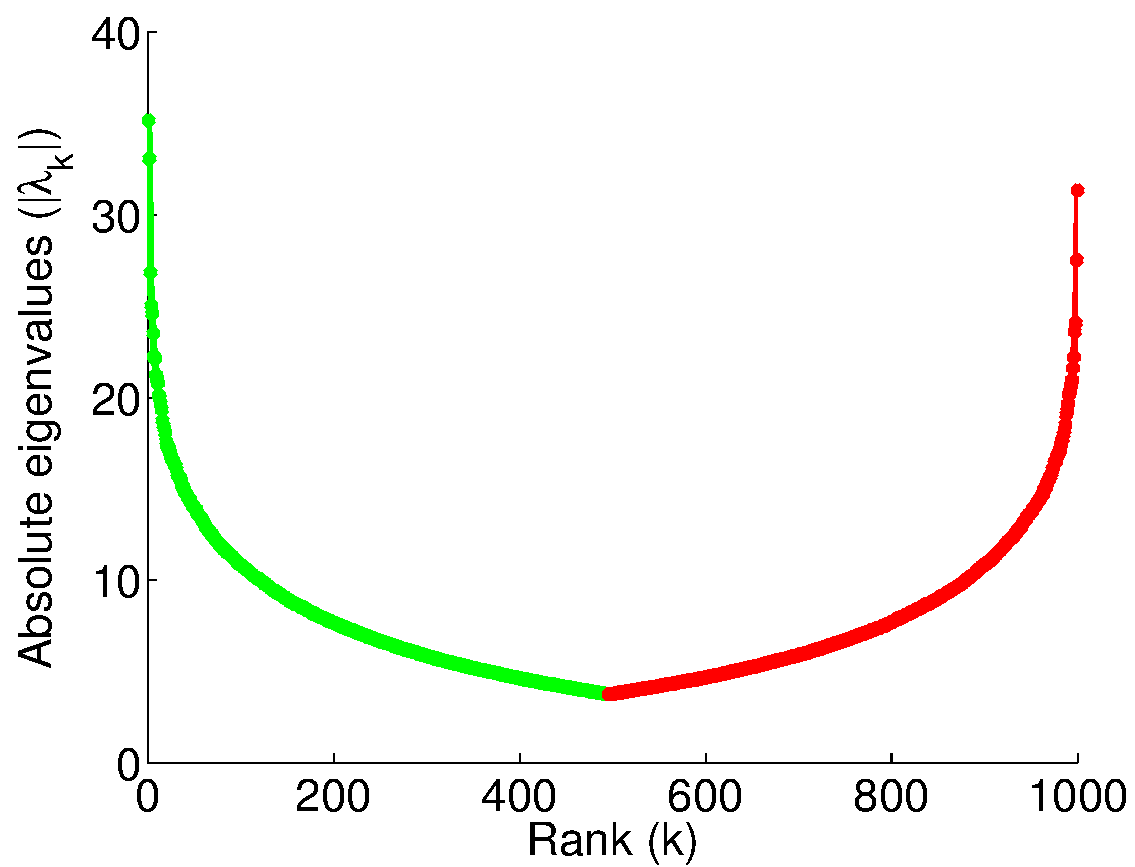
\includegraphics[width=\wPlot]{plot/decomposition.b.sym.elec}}
  \subfigure[Cumulative eigenvalue distribution of $\mathbf N$]{
    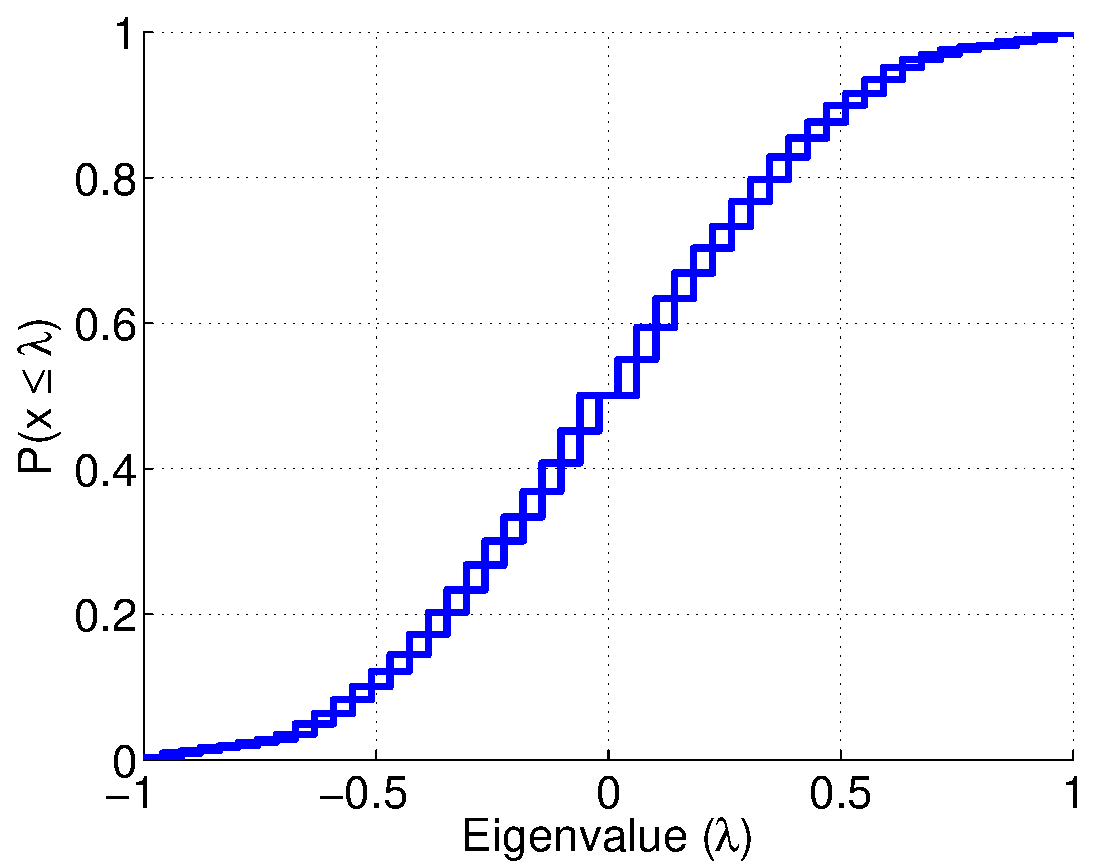
\includegraphics[width=\wPlot]{plot/distr.f.sym-n.elec}}
  \caption{ The top-$k$ eigenvalues of $\mathbf A$ and the cumulative
    spectral distribution of $\mathbf N$ for the Wikipedia election
    network
    (\href{http://konect.uni-koblenz.de/networks/elec}{\textsf{EL}}).
    In the first plot~(a), positive eigenvalues are shown in green and
    negative ones in red.
    \label{fig:spectrum}
  }
\end{figure}

Two plots are generated: the non-cumulative eigenvalue distribution, and
the cumulative eigenvalue distribution.  For the non-cumulative
distribution, the absolute $\lambda_i$ are shown in function of $i$ for
$1 \leq i \leq k$.  The sign of eigenvalues (positive and negative) is
shown by the color of the points (green and red).  For the cumulated
eigenvalue plots, the range of all eigenvalues is computed, divided into
49 bins (an odd number to avoid a bin limit at zero for the matrix
$\mathbf N$), and then the number of eigenvalues in each bin is
computed.  The result is plotted as a cumulated distribution plot, with
boxes indicating the uncertainty of the computation, due to the fact
that eigenvalues are not computed exactly, but only in bins.

\subsection{Complex Eigenvalues Plot}
The adjacency matrix of an undirected graph is symmetric and therefore
its eigenvalues are real.  For directed graphs however, the adjacency
matrix $\mathbf A$ is asymmetric, and in the general case its
eigenvalues are complex.  We thus plot, for directed graphs, the top-$k$
complex eigenvalues by absolute value of the adjacency matrix $\mathbf
A$.

Three properties can be read off the complex eigenvalues: whether a graph
is nearly acyclic, whether a graph is nearly symmetric, and whether a
graph is nearly bipartite.  If a  
directed graph is acyclic, its adjacency matrix is nilpotent and
therefore all its eigenvalues are zero. The complex eigenvalue plot can
therefore serve as a test for networks that are nearly acyclic: the
smaller the absolute value of the complex eigenvalues of a directed
graph, the nearer it is to being acyclic.  When a directed network is
symmetric, i.e., all directed edges come in pairs connecting two nodes
in opposite direction, then the adjacency matrix $\mathbf A$ is
symmetric and therefore all its eigenvalues are complex. Thus, a nearly
symmetric directed network has complex eigenvalues that are near the
real line.  
Finally, the eigenvalues of a bipartite graph are symmetric around the
imaginary axis.  In other words, if $a+bi$ is an eigenvalue, then so
is $-a+bi$ when the graph is bipartite.  Thus, the amount of symmetric
along the imaginary axis is an indicator for bipartivity. Note that
bipartivity here takes into account edge directions:  There must be two
groups such that all (or most) directed edges go from the first group to
second. 
Figure~\ref{fig:complex} shows two examples of such plots.

\begin{figure}
  \centering \subfigure[Wikipedia elections]{
    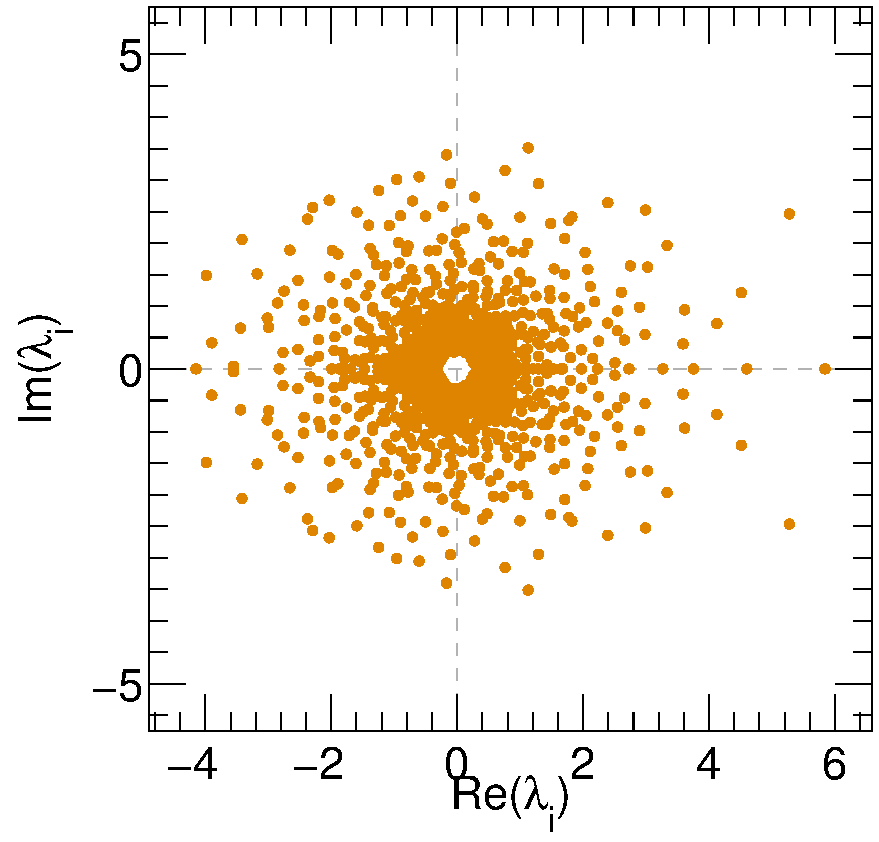
\includegraphics[width=\wTwo]{plot/decomposition.complex.diag.elec}}
  \subfigure[UC Irvine messages]{
    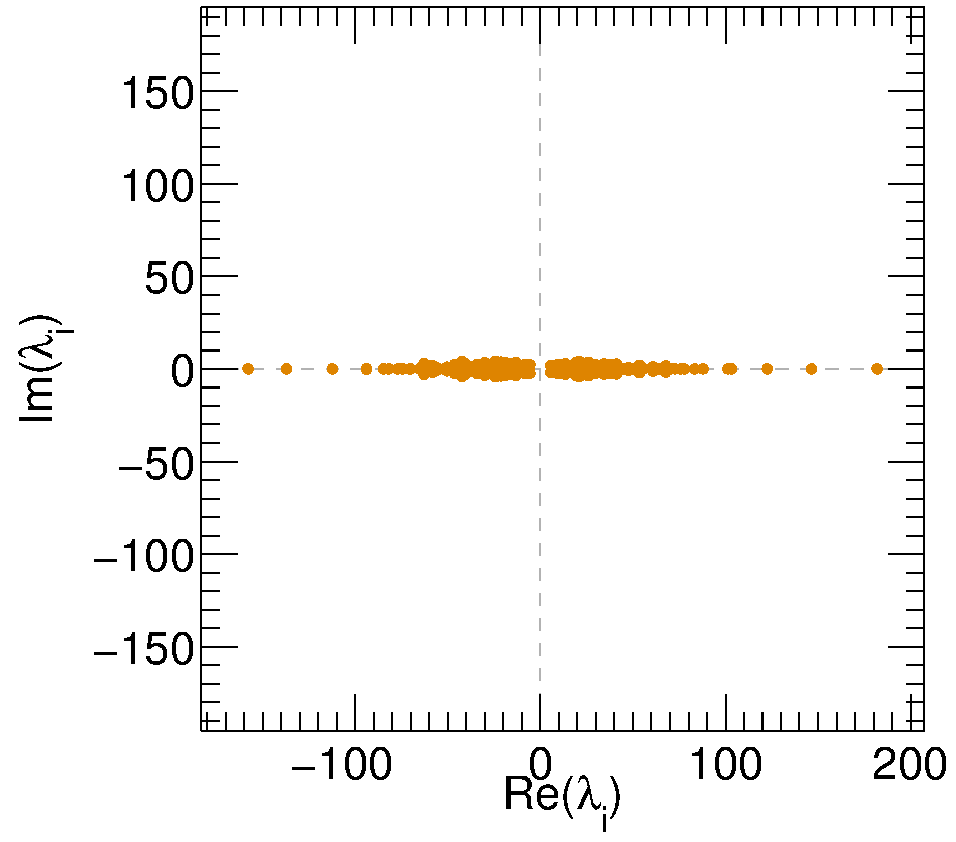
\includegraphics[width=\wTwo]{plot/decomposition.complex.diag.opsahl-ucsocial}}
  \caption{ The top-$k$ complex eigenvalues $\lambda_i$ of the
    asymmetric adjacency matrix $\mathbf A$ of the directed Wikipedia
    election~(\href{http://konect.uni-koblenz.de/networks/elec}{EL}) and
    UC Irvine
    messages~(\href{http://konect.uni-koblenz.de/networks/opsahl-ucsocial}{UC})
    networks.
    \label{fig:complex}
  }
\end{figure}

\subsection{Distance Distribution Plot}
Distance statistics can be visualized in the distance distribution plot.
The distance distribution plot shows, for each integer $k$, the number
of node pairs at distance $k$ from each other, divided by the total
number of node pairs.  The distance distribution plot is also called the
\emph{hop plot}.  
The distance distribution plot can be used to
read off the diameter, the median path length, and the 90-percentile
effective diameter (see Section~\ref{sec:distance-statistics}).  For
temporal networks, the distance distribution plot can be shown over
time.

The non-temporal distance distribution plot shows the cumulated distance
distribution function between all node pairs $(u,v)$ in the network,
including pairs of the form $(u,u)$, whose distance is zero.

The temporal distance distribution plot shows the same data in function
of time, with time on the X axis, and each colored curve representing
one distance value.

\begin{figure}
  \centering \subfigure[Distance distribution plot]{
    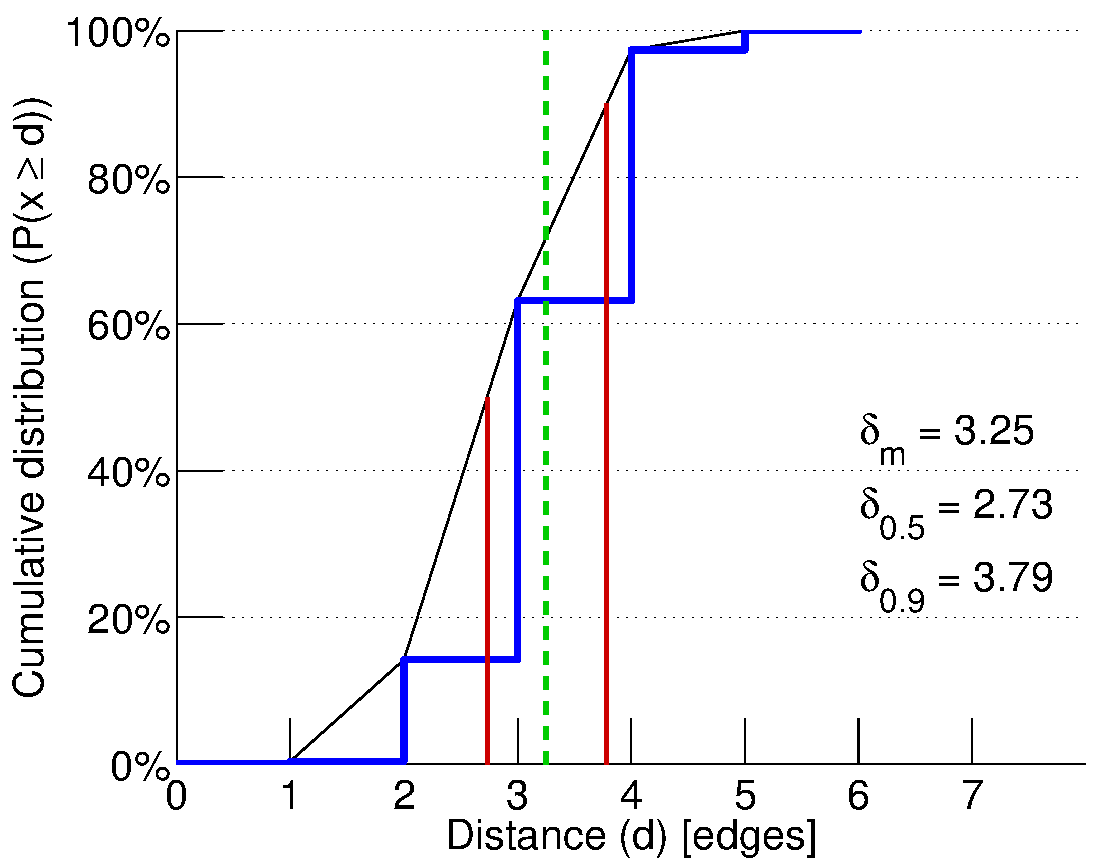
\includegraphics[width=\wPlot]{plot/hopdistr.a.elec}}
  \subfigure[Temporal distance distribution plot]{
    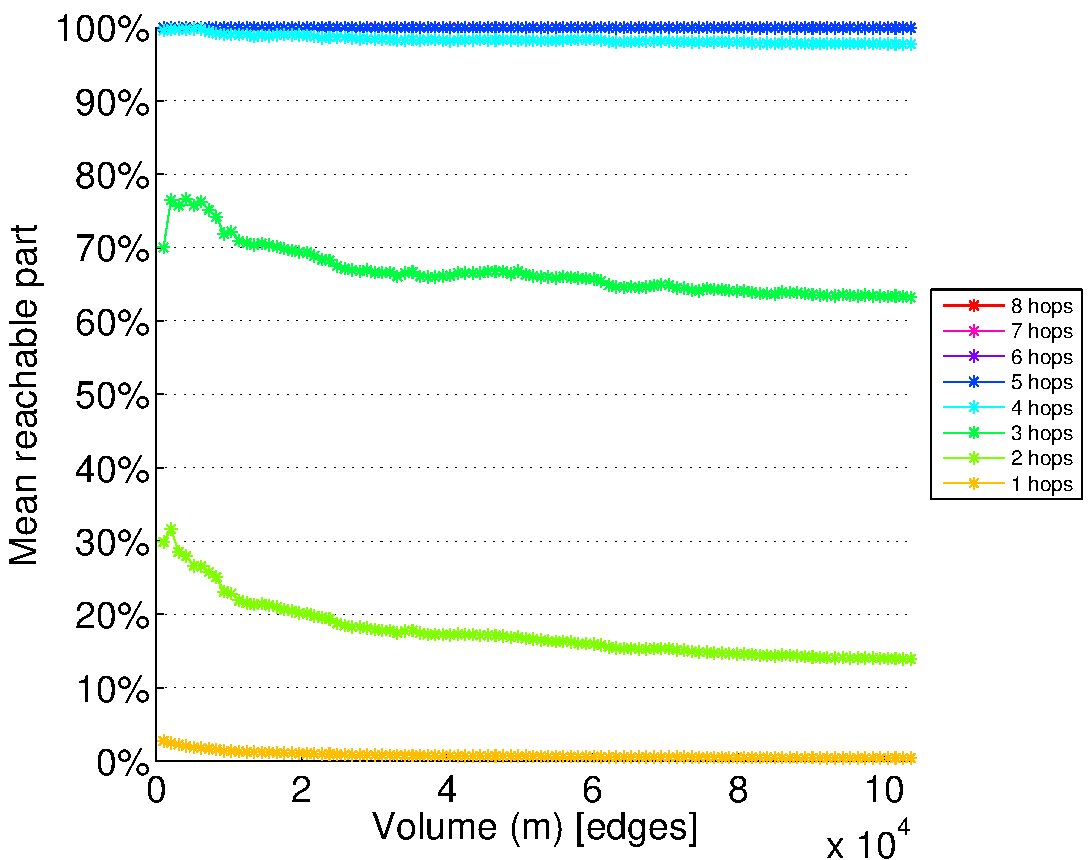
\includegraphics[width=\wPlot]{plot/hopdistr_time.full.c.elec}}
  \caption{ The distance distribution plot and temporal distance
    distribution plot of the Wikipedia election network
    (\href{http://konect.uni-koblenz.de/networks/elec}{\textsf{EL}}).
    \label{fig:hopdistr}
  }
\end{figure}

\subsection{Graph Drawings}
A graph drawing is a representation of a graph, showing its vertices and
egdes laid out in two (or three) dimensions in order for the graph
structure to become visible.  Graph drawings are easy to produce when a
graph is small, and become harder to generate and less useful when a
graph is larger.

Given a graph, a graph drawing can be specified by the placement of its
vertices in the plane.  To determine such a placement is a non-trivial
problem, for which many algortihms exist, depending on the required
properties of the drawing. For instance, each vertex should be placed
near to its neighbors, vertices should not be drawn to near to each
other, and edges should, if possible, not cross each other.  It is clear
that it is impossible to fulfill all these requirements at once, and
thus no best graph drawing exists.

In KONECT, we show drawings of small graphs only, such that vertices and
edges remain visible. The graph drawings in KONECT are spectral graph
drawings, i.e., they are based on the eigenvectors of characteric graph
matrices.  In particular, KONECT included graph drawings based on the
adjacency matrix $\mathbf A$, the normalized adjacency matrix $\mathbf
N$ and the Laplacian matrix $\mathbf L$ \citep{b405}. Let $\mathbf x$ and $\mathbf y$
be the two chosen eigenvector of each matrix, then the coordinate of the
node $u\in V$ is given by $\mathbf x_u$ and $\mathbf y_u$.

For the adjacency matrix $\mathbf A$ and the normalized adjacency matrix
$\mathbf N$, we use the two eigenvector with largest absolute eigevalue.
For the Laplacian matrix $\mathbf L$, we use the two eigenvectors with
smallest nonzero eigenvalue.  Examples for the Zachary karate club
social network
(\href{http://konect.uni-koblenz.de/networks/ucidata-zachary}{\textsf{ZA}})
are shown in Figure~\ref{fig:map.ax}.

\begin{figure}
  \centering \subfigure[Adjacency matrix~$\mathbf A$]{
    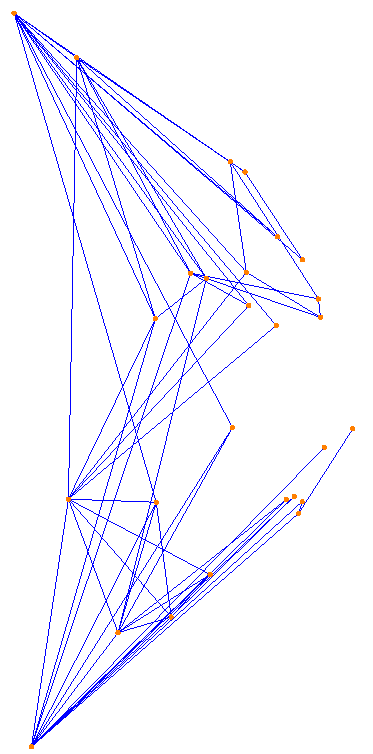
\includegraphics[width=\wFour]{plot/map.ax.sym.ucidata-zachary}}
  \subfigure[Normalized adjacency matrix~$\mathbf N$]{
    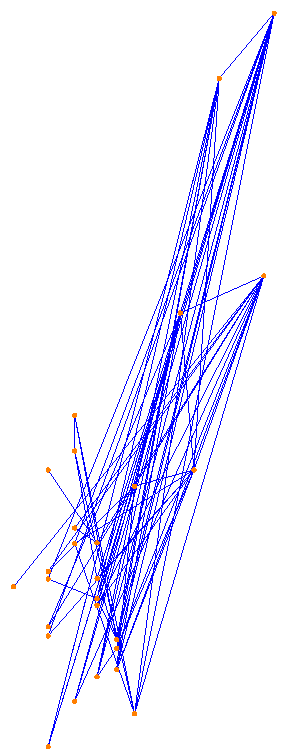
\includegraphics[width=\wFour]{plot/map.ax.sym-n.ucidata-zachary}}
  \subfigure[Laplacian $\mathbf L$]{
    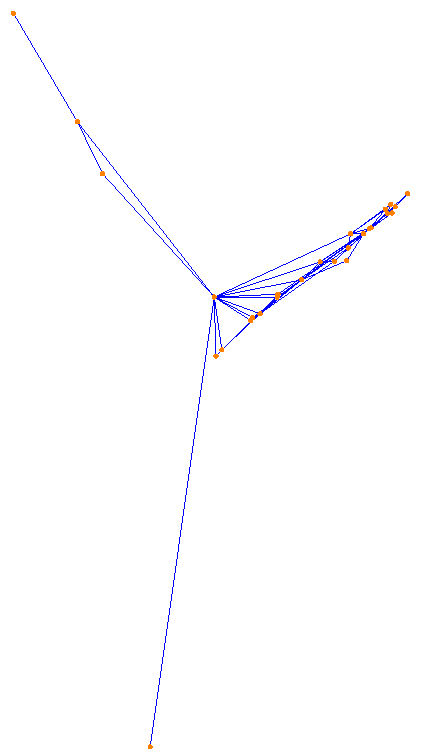
\includegraphics[width=\wFour]{plot/map.ax.lap.ucidata-zachary}}
  \caption{ Drawings of the Zachary karate club social network
    (\href{http://konect.uni-koblenz.de/networks/ucidata-zachary}{\textsf{ZA}})
    using (a)~the adjacency matrix~$\mathbf A$, (b)~the normalized
    adjacency matrix~$\mathbf N$, (c)~the Laplacian matrix~$\mathbf L$.
    \label{fig:map.ax}
  }
\end{figure}

\section{The KONECT Toolbox}
\label{sec:toolbox}
The KONECT
Toolbox\footnote{\href{https://github.com/kunegis/konect-toolbox}{https://github.com/kunegis/konect-toolbox}}
for Matlab is a set of functions for the Matlab programming
language\footnote{\href{http://www.mathworks.com/products/matlab/}{www.mathworks.com/products/matlab}}
containing implementations of statistics, plots and other network
analysis methods.  The KONECT Toolbox is used to generate the numerical
statistics and plots in this handbook as well as on the KONECT website.

\paragraph{Installation}
The KONECT Toolbox is provided as a directory containing *.m files.  The
directory can be added to the Matlab path using addpath() to be used.

\paragraph{Usage}
All functions have names beginning with \texttt{konect\_}.

\subsection{Examples}
This section gives short example for using the toolbox.  The examples
can be executed in Matlab. 

\paragraph{Load a unipartite dataset}
This example loads the Slashdot signed social network. 

\begin{verbatim}
T = load('out.slashdot-zoo');
n = max(max(T(:,1:2)));
A = sparse(T(:,1), T(:,2), T(:,3), n, n); 
\end{verbatim}

This loads the weighted adjacency matrix of the Slashdot Zoo into the
matrix \texttt{A}. 

\subsection{Variables}
Naming variables can be quite complicated and hard to read in
Matlab. Therefore KONECT code follows these rules.

Long variable names (containing full words) are in all-lowercase. Words
are separated by underscore.  When refering to a variable in comments,
the variable is written in all-uppercase.  Short variable names
(letters) are lowercase for numbers and vectors, and uppercase for
matrices.

\subsubsection{Strings}
Table~\ref{tab:string-variables} shows common variable names used for
string variables.

\begin{table}
  \caption{ 
    Long variable names of string type used in KONECT.
    \label{tab:string-variables}
  } 
  \centering
  \begin{tabular}{>{\ttfamily}lp{0.7\textwidth}}
    \toprule 
    network & The internal network name, e.g., ``advogato''.
    The internal network name is used in the names of files related to
    the network. \\ 

    class &
    The internal name for a set of networks, e.g., ``test'', ``1'',
    ``2'', ``3''. The class ``N'' includes the $10\times N$ smallest
    networks. \\ 
    code & The 1/2/3-character code for a network, e.g.,
    ``EN'' for Enron.  \\ 
    curve & The internal name of a curve fitting method. \\ 
    decomposition & The internal of a matrix decomposition, as passed to the function
    \texttt{konect\_decomposition()}, e.g., ``sym'', ``asym'' and ``lap''. \\ 
    feature & The internal name of a
    feature, e.g., ``degree'' and ``decomp.sym''.  \\ 
    filename & A filename. \\ 
    format & The network format in lower case as defined in
    the function \texttt{konect\_consts()}, e.g., ``sym'' and ``bip''. \\ 
    label &
    The readable name of things used in plots, tables, etc.  \\ 
    measure & The internal name of a measure
    of link prediction accuracy, e.g., ``map'' and ``auc''. \\ 
    method & The internal name of a
    link prediction method.  \\ 
    statistic & The internal name of a network
    statistic, e.g., ``power'' and ``alcon''.  \\ 
    transform & The name of a transform, e.g. ``simple'' and ``lcc''. \\
    type & The internal name of
    the computation type. This can be ``split'' or ``full''. This
    decides which version of a network gets used, in particular for
    time-dependent analyses.  \\ 
    weights & The edge weight type as defined in the function
    \texttt{konect\_consts()}, e.g., ``unweighted'' and
    ``signed''. \\ 

    \bottomrule
\end{tabular}
\end{table}

\subsubsection{Scalars}
Table~\ref{tab:scalar-variables} shows variable names used for scalar
values.

\begin{table}
  \caption{ Variable names used for scalars in KONECT.
    \label{tab:scalar-variables}
  } \centering
  \begin{tabular}{>{\ttfamily}lp{0.7\textwidth}}
    \toprule n, n1, n2 & Row/column count in matrices, left/right vertex
    count \\ r & Rank of a decomposition \\ m & Edge count \\ i, j &
    Vertices as integer, i.e., indexes in rows and
    columns. \\ prediction & A link prediction score, i.e., a value
    returned by a link prediction algorithm for a given node
    pair. \\ precision & The prediction accuracy value, typically
    between 0 and 1.  \\ means & Values used for additive
    (de)normalization, as a structure. \\ \bottomrule
  \end{tabular}
\end{table}

\subsubsection{Matrices}
Table~\ref{tab:matrix-variables} shows variable names used for
matrix-valued variables.

Note that when the adjacency matrix of an undirected graph is stored in
a variable, each edge is usually stored just once, instead of twice. In
other words, the variable \texttt{A} for undirected networks does not
equal the matrix $\mathbf A$, instead the expression \texttt{A + A'}
does.

\begin{table}[h]
  \caption{ 
    Variable names used for matrices and vectors in KONECT.
    As a general rule, matrices have upper-case names and vectors have
    lower-case names. 
    \label{tab:matrix-variables}
  } 
  \centering
  \begin{tabular}{>{\ttfamily}lp{0.7\textwidth}}
    \toprule 
    A & ($n \times n$) Adjacency matrix (in code where the
    adjacency and biadjacency matrix are distinguished) \\ 
    A & ($n \times n$ or $n_1 \times n_2$) Adjacency or biadjacency matrix (in
    code where the two are not distinguished) \\ 
    B & ($n_1 \times n_2$) Biadjacency matrix
    (in code where the adjacency and biadjacency matrix are
    distinguished) \\ 
    D & ($r \times r$) Central matrix; e.g.,
    eigenvalues; as matrix \\ 
    dd & ($r \times 1$) Diagonal of the
    central matrix \\ 
    E & ($e \times 2$) Test set for link prediction, stored in the same
    way as \texttt{T} \\
    L & ($n \times n$) Laplacian matrix \\ 
    M, N &
    Normalized (bi)adjacency matrix \\ 
    T & ($m \times 2$ or
    $m \times 3$ or $m \times 4$) Compact adjacency matrix, as stored in
    \texttt{out.*} files, and such that it can be converted to a sparse
    matrix using \texttt{konect\_spconvert()}. \\ 
    & First column: row
    IDs \\ 
    & Second column: column IDs \\ 
    & Third column (optional):
    edge weights (1 if not present) \\ 
    & Fourth column (optional):
    timestamps in Unix time \\ 
    U & ($n \times r$ or $n_1 \times
    r$) Left part of decomposition; e.g., left eigenvectors \\ 
    V & ($n
    \times r$ or $n_2 \times r$) Right part of decomposition; e.g.,
    right eigenvectors \\ 
    X & ($r \times r$) Central matrix, when
    explicitly nondiagonal \\ 
    Z & ($n \times n$) Normalized Laplacian
    matrix \\ 
    \bottomrule
\end{tabular}
\end{table}

\subsubsection{Compound Types}

A struct containing elements whose names are of a specific type are
named \texttt{[VALUETYPE]s\_[KEYTYPE]}.  For instance, a struct with
labels used for methods is named as follows:

\begin{verbatim}
labels_method.('auc') = 'Area under the curve';
\end{verbatim}

Note:
\begin{itemize}
\item The first element is the name of the content type.
\item The plural is used only for the content type.
\end{itemize}

\subsubsection{IDs}

Variables named \texttt{method}, \texttt{decomposition}, etc.\ are
always strings.  If a method, decomposition or any other type is
represented as an integer (e.g., as an index into an array), then
\texttt{\_id} is appended to the variable name. For instance:

\begin{verbatim}
decomposition = 'sym'; decomposition_id = 2;
\end{verbatim}

This means that an array of values by ID of keys is called for instance:

\begin{verbatim}
labels_decomposition_id{1} = 'Eigenvalue decomposition';
labels_decomposition_id{2} = 'Singular value decomposition';
\end{verbatim}

\section{File Formats}
\label{sec:format}
Due to the ubiquity of networks in many areas, there are a large number
of file formats for storing graphs and graph-like structures.  Some of
these are well-suited for accessibility from many different programming
languages (mostly line-oriented text formats), some are well-suited for
integration with other formats (semantic formats such as RDF and
XML-based ones), while other formats are optimized for efficient access
(binary formats).  In KONECT, we thus use three file formats covering
the three cases:
\begin{itemize}
\item TSV format: This format is text-based and uses tab- or space-separated 
  values.  This is the main KONECT data format from which the two others
  are derived.  The format has the advantage that it can be read easily
  from many different programming languages and environments.
\item RDF format: Datasets are also available as RDF.  This is intended
  for easy integration with other datasets.  This format is deprecated
  as it did not have any users. 
\item Matlab format: To compute statistics and plots and perform
  experiments, we use Matlab's own binary format (version 7.3), which can be accessed
  efficiently from within Matlab.
\end{itemize}

\subsection{TSV Format}
In the following, we describe KONECT's TSV format.  Each network
\texttt{\$NETWORK} is represented by the file \texttt{out.\$NETWORK}. 

The edges stored as tab separated values (TSV).  The file is a text
file, and each line contains information about one edge.  Each line
contains two, three or four numbers represented textually, and separated
by any sequence of whitespace.  The preferred separator is a single tab.
The first two columns are mandatory and contain the source and
destination node ID of the edge.  The third column is optional and
contains the edge weight.  When the network is dynamic, the third column
contains $+1$ for added edges and $-1$ for removed edges.  For
unweighted, non-temporal networks, multiple edges may be aggregated into
a single line containing, in the third column, the number of aggregated
edges.  The fourth column is optional and contains the edge creation
time, and is stored as UNIX time, i.e., the number of seconds since 1
January 1970.  The fourth column is usually an integer, but may contain
floating point numbers.  If the fourth column is present, the third
column must also be given.  The beginning of the file contains
additional comment lines with the following information:
\begin{verbatim}
   % FORMAT WEIGHTS 
   % RELATIONSHIP-COUNT SUBJECT-COUNT OBJECT-COUNT
\end{verbatim}
where \texttt{FORMAT} is the internal name for the format as given
in Table~\ref{tab:format}, \texttt{WEIGHTS} is the internal name for
the weight types as given in Table~\ref{tab:weights},
\texttt{RELATIONSHIP-COUNT} is the number of data lines in the file,
and \texttt{SUBJECT-COUNT} and \texttt{OBJECT-COUNT} both equal the
number of nodes $n$ in unipartite networks, and the number of left
and right nodes $n_1$ and $n_2$ in bipartite networks.  The first
line is mandatory; the second line is optional.

\subsection{Meta File}
In addition to the data files (TSV, etc.), each network in KONECT has a
file \texttt{meta.\$NETWORK} associated with it.  This is a short text
file that contains all information about the dataset that are not
structural.  In other words, all structural information is stored in the
TSV and other data formats, while meta information is stored in this
file. 
The file contains metadata about the
network that is independent of the mathematical structure of the
network.  
The file is a text file coded in UTF-8.  Each line
contains one key/value pair, written as the key, a colon and the
value.  The following metadata are used:
\begin{itemize}
\item \texttt{name}: The name of the dataset.  This contains only the
  name of the source, without description the type or category,
  e.g., ``YouTube'', ``Wikipedia elections'').  The name uses
  sentence case.  For networks with the same name the source (e.g.,
  the conference) is added in parentheses.  Within each category,
  all names must be distinct, but multiple networks can have the same
  \texttt{name} if they have different categories. 
\item \texttt{code}: The short code used in plots and narrow
  tables.  The code consists of two or three alphanumeric characters.  The first
  two characters are usually uppercase letters and denote the data
  source.  The last character, if present, usually distinguishes
  the different networks from one source.  The code is unique across all
  of KONECT, although it is not an error if they are not:  It will only
  lead to certain plots be confusing. 
\item \texttt{url}: (optional) The URL(s) of the data sources, as a comma
  separated list.  Most datasets have a single URL.
\item \texttt{category}: The name of the category, as given in the
  column ``Category'' in Table~\ref{tab:categories}.
\item \texttt{description}: (deprecated) A short description of the form
  ``User–movie ratings''.  Note that the file should contain an
  actual en dash, coded in UTF-8.
\item \texttt{cite}: (optional) The bibtex key of the citation(s) for this dataset, as a
  comma separated list. Most dataset have a single bibtex entry.  This
  is usually the actual paper about the dataset.  Many researchers have
  a preference about which of their papers should be cited for a dataset
  they have released, and we follow these. 
\item \texttt{fullname}: (optional) A longer name to disambiguate
  different datasets from the same source, e.g., ``Youtube
  ratings'' and ``Youtube friendships''.  Uses sentence case.  These
  names are unique across KONECT, falling back to the \texttt{name} when
  the fullname is not given. 
\item \texttt{long-description}: (optional, recommended) A long descriptive
  text consisting of full sentences, and describing the dataset in
  a verbose way.  HTML markup may be used sparingly (tags: I,
  etc.), usually only for absolutely necessary typography, such as
  setting species names in italics.  Hyperlinks are not used. 
\item \texttt{entity-names}: A comma-seperated list of
  entity names (e.g., ``user, movie'').  Unipartite networks give
  a single name; bipartite networks give two.
\item \texttt{relationship-names}: The name of the
  relationship represented by edges, as a substantive (e.g.,
  ``friendship'').
\item \texttt{extr}: (optional, recommended) The name of the
  subdirectory of \texttt{konect-extr/extr/} that
  contains the extraction code for this dataset.
\item \texttt{timeiso}: (optional) A single ISO timestamp denoting
  the date of the dataset or two timestamps separated by a
  slash(/) for a time range. The format is:
  YYYY[-MM[-DD]][/YYYY[-MM[-DD]]], e.g., ``2005-10-08/2006-11-03''
  or ``2007''.
\item \texttt{tags}: (optional) A space-separated list of hashtags
  describing the network.  The list of tags is given in
  Section~\ref{sec:tags}.  
\item \texttt{n3-*}: (optional, deprecated) Metadata which is used for the
  generation of RDF files. The symbol \texttt{\{n\}} in the name
  of the meta key represents an order by unique, sequential
  numbers starting at 1.
  \begin{itemize}
  \item \texttt{n3-add-prefix\{n\}} (optional):
    Used to define additional N3 prefixes. The
    default prefixes are specified in this way.
  \item \texttt{n3-comment-\{n\}} (optional): Add
    commentary lines which are placed at the
    beginning of the N3 file.
  \item \texttt{n3-edgedata-\{n\}} (optional):
    Additional N3-data, to be displayed with each
    edge.
  \item \texttt{n3-nodedata-m-\{n\}} (optional):
    Additional N3-data, to be displayed with the
    first occurence of the source ID.
  \item \texttt{n3-nodedata-n-\{n\}} (optional):
    Additional N3-data, to be displayed with the
    first occurence of the target ID.
  \item \texttt{n3-prefix-m}: N3-prefix for the
    source IDs.
  \item \texttt{n3-prefix-n} (optional): N3-prefix
    for the target IDs. If this field is left out,
    the value of \{n3-prefix-m\} is used.
  \item \texttt{n3-prefix-j} (optional):
    Additional prefix which can be used with the
    source id, if there is an entity to be
    represented with the same id.
  \item \texttt{n3-prefix-k} (optional):
    Additional prefix which can be used with the
    target id, if there is an entity to be
    represented with the same id. This is used for
    example in meta.facebook-wosn-wall for the
    representation of users walls.
  \item \texttt{n3-prefix-l} (optional): N3-prefix
    for the edges, if they are to be represented
    by some N3-entity.
  \item \texttt{n3-type-l} (optional): RDF-type
    for the edges.
  \item \texttt{n3-type-m}: RDF-type for source
    IDs.
  \item \texttt{n3-type-n} (optional): RDF-type
    for target IDs.
  \end{itemize}
  The following symbols are used in the n3-expressions for
  edgedata and nodedata:
  \begin{itemize}
  \item[\texttt{\$m}]: n3-prefix-m + source ID
  \item[\texttt{\$n}]: n3-prefix-n (or n3-prefix-m
    if the other is undefined) + target ID
  \item[\texttt{\$j}]: source ID
  \item[\texttt{\$k}]: target ID
  \item[\texttt{\$l}]: edge ID
  \item[\texttt{\$timestamp}]: edge timestamp
  \end{itemize}
\end{itemize}

\section*{Acknowledgments}
The KONECT project would not have been possible without the
effort of many people who have made datasets available and also helped
the project in other ways.   
KONECT is maintained by Jérôme Kunegis (University of Namur). 
In the past, KONECT was also maintained by Daniel Dünker, Holger Heinz,
and Martina Sekulla (University of Koblenz--Landau). 

We owe much of the datasets in KONECT to researchers of many different
fields of science from all around the world who contributed datasets to
the public, and to KONECT in particular.  The list of contributors would
be too long to list, so instead we refer to the online list of datasets
for links to dataset sources and citations relevant to each
network.\footnote{\url{http://konect.uni-koblenz.de/networks/}}

KONECT was also supported by funding from multiple research projects. 
The research leading to
these results has received funding from the European Community's Seventh
Frame Programme under grant agreements n\textsuperscript{o}~257859,
\href{http://robust-project.eu/}{ROBUST}, 287975,
\href{http://www.socialsensor.eu/}{SocialSensor}, and 610928,
\href{http://revealproject.eu/}{REVEAL}, as well as the project
\href{http://nouvelles.unamur.be/upnews.2015-10-01.8995593781}{IDEES --
  L'Internet de Demain pour développer les Entreprises, l'Économie et la
  Société} (ERDF/FEDER -- Wallonia/Wallonie). 

The picture of a pair of cherries in Figure~\ref{fig:cherries} was
created by the authors of Wikimedia Commons and is released under the
Creative Commons CC-SA~3.0 license.\footnote{\url{https://commons.wikimedia.org/wiki/File:Cherry_Stella444.jpg}}

\let\oldbibliography\thebibliography
\renewcommand{\thebibliography}[1]{%
  \oldbibliography{#1}%
  \setlength{\itemsep}{0pt}%
}
\bibliographystyle{agsm}
\bibliography{kunegis,ref,konect}

\appendix

\section{Glossary of Terms}

Some terms related to graph theory are well established in mathematics,
network theory and computer science, while other terms do not have a
widely-used definition.  
The choices made in this work are those of the authors, and were chosen
to reflect best practices and to avoid confusion.

\begin{description}
  \item[Adjacency matrix]
    The matrix describing a network, usually denoted $\mathbf A$.  To be
    contrasted with the 
    half-adjacency matrix (for undirected unipartite networks, also
    denoted $\mathbf A$) and the
    biadjacency matrix (for bipartite networks, denoted $\mathbf B$). 
    The adjacency matrix is always square, and for undirected networks
    it is symmetric. 
  \item[Arc] A directed edge.  In general, we consider arcs to be a
    special cases of edges, and thus we rarely use the term \emph{arc}
    in favor of \emph{directed edge}.  (In other texts, an edge is taken
    to be undirected by definition, and the term \emph{directed edge} is
    then a contradiction.)
  \item[Biadjacency matrix]
    The characteristic matrix of a bipartite network, usually denoted
    $\mathbf B$.  The corresponding adjacency matrix is then $[\mathbf
      0, \mathbf B; \mathbf B^{\mathrm T}, \mathbf 0]$. 
  \item[Category] Networks have a category, which describes the domain
    they apply to:  social networks, transport networks, citation
    networks, etc. 
  \item[Central matrix] The matrix $\mathbf X$ in any decomposition
    of the form $\mathbf U \mathbf X \mathbf V^{\mathrm T}$, not necessarily
    diagonal or symmetric; a generalization of the diagonal eigenvalue
    matrix.
  \item[Class]
    The networks of KONECT are divided into classes by their volume:
    Class~1 contains the ten smallest networks, Class~2 contains the
    next ten smallest networks, etc.  
  \item[Claw]
    Three edges sharing a single vertex.  A claw can be understood as a 3-star. 
  \item[Code]
    The two- or three-character code representation of a network.  These
    are used in scatter plots that show many networks.  
  \item[Cross]
    A pattern of four edges sharing a single endpoint.  Also called a
    4-star.  
  \item[Curve]
    A curve fitting method used for link prediction, when using the link
    prediction method described
    in \citep{kunegis:spectral-transformation}.
  \item[Cycle] 
    A cyclic sequence of connected edges, not containing any edge twice.
    A cycle contrasts with a tour, in which a single vertex can appear
    multiple times.  
  \item[Decomposition] In KONECT the word \emph{decomposition} is used
    to denote the combination of a characteristic graph matrix (e.g. the
    adjacency matrix or Laplacian) with a matrix decomposition.  As an
    extension, some other constructions are also called
    \emph{decomposition}, such as LDA.
  \item[Density] This word is avoided in KONECT.  In the literature, it
    may refer to either the fill (probability that an edge exists), or to
    the average degree.  The former definition is typically used in mathematical
    contexts, while the latter is used in computer science contexts.
  \item[Edge] A connection between two nodes.  In mathematics, an edge
    is undirected and constrasts with an arc which is directed.  In the
    context of KONECT, all types of connections between nodes are called
    \emph{edges} and an arc is a special case of an edge. 
  \item[Feature] A node feature. I.e., a number assigned to each node.
    Examples are the degree, PageRank and the eccentricity. 
    Equivalently, a node vector.
  \item[Fill] The probability that two randomly chosen nodes are
    connected.  Also called the \emph{density}, in particular in a
    mathematical context.  The fill is the sole parameter of the
    Erdős--Rényi random graph model.  The word \emph{fill} is specific
    to KONECT. 
  \item[Format] 
    The format of a network determines its general structure, and
    whether edges are directed.  There are three possible formats:
    unipartite and undirected; unipartite and directed; and bipartite.
    Directed bipartite networks are not possible in KONECT.  Possible future
    extensions would include hypergraphs (e.g., tripartite networks).  
  \item[Half-adjacency matrix]
    The adjacency matrix $\mathbf A$ of an undirected graph contains two
    nonzero entries for each edge $\{i,j\}$:  $\mathbf A_{ij}$ and
    $\mathbf A_{ji}$.  To avoid this, KONECT code uses the
    half-adjacency matrix, which contains only one of the two nonzero
    entries.  The half-adjacency matrix is therefore not unique, i.e.,
    it is unspecified whether $\mathbf A_{ij}$ or $\mathbf A_{ji}$ is nonzero.  In
    code, the half-adjacency matrix is denoted \texttt{A}.  The term
    \emph{half-adjacency matrix} is specific to KONECT, but the use of
    such a representation is widespread. 
  \item[Measure]
    A measure of the accuracy of link prediction methods, for instance
    the area under the curve or the mean average precision.  
  \item[Method]
    A link prediction method. 
  \item[PageRank] 
    A node-based feature of a directed network, defined as the dominant
    eigenvector of the matrix $\mathbf G = (1-\alpha) \mathbf P +
    \alpha\mathbf J$, with eigenvalue one. 
  \item[Path]
    A sequence of connected nodes, in which each node can appear only
    once.  The extension that allows multiple nodes is called a walk.  A
    path with identical start and end nodes is called a \emph{cycle}. 
  \item[Score]
    A numerical value given to a node pair.  Usually used for link
    prediction, but can also measure distance or similary between
    nodes. 
  \item[Size]
    The number of nodes in a network.  
  \item[Statistic]
    A statistic is a numerical measure of a network, i.e., a number that
    describes a network, such as the clustering coefficient, the
    diameter or the algebraic connectivity.  All statistics are real
    numbers.   
  \item[Tour]
    A cyclic sequence of connected nodes which may contain a single
    vertex multiple times.  It can be considered a walk that returns to
    it starting point, or a generalization of a cycle that allows to
    visit nodes multiple times.  
  \item[Transform] 
    A transform is an operation that applies to a graph and that gives
    another graph.  Examples are taking the largest connected component,
    removing multiple edges, and making a bipartite graph unipartite.
    Certain graph properties can be expressed as other graph properties
    applied to graph transforms.  For instance, the size of the largest
    connected component is the size of the transform which keeps only
    the largest connected component. 
  \item[Triangle]
    Three nodes all connected with each other.  The number of triangles
    in a network is a commonly used statistic, used for instance as
    the basis to compute the clustering coefficient.  Counting the
    triangles in a network is a very common computational problem.  
  \item[Volume]
    The number of edges in a network.  
  \item[Walk]
    A sequence of connected nodes, which may contain a single node
    multiple times.  The restriction to include a single node only once
    is called a path.  If the endpoints of a walk are identical, then
    the walk is also a tour.  
  \item[Wedge] 
    Two edges sharing a common node, i.e., two incident edges.  The
    number of wedges in a network is an important network statistic,
    which characterizes that skewness of the degree distribution, and
    which can be easily calculated.  A wedge can be seen as a 2-star or
    a 2-path.  
  \item[Weights] (always in the plural)
    The weights of a network describe the range of edge weights it
    allows.  The list of possible edge weights is given in
    Table~\ref{tab:weights}.  
\end{description}

\section{Glossary of Mathematical Symbols}

The following symbols are used in mathematical expessions throughout
KONECT.  Due to the large number of different measures used in graph
theory and network analysis, many common symbols for measures overlap.
For many measures, there is more than one commonly-used notation; the
notation chosen in KONECT represents a reasonable balance between using established
notation when it exists, and having distinct symbols for different
measures. \\

\begin{longtable}{ll}
  \toprule
  \textbf{Symbol} & \textbf{Meaning} \\
  \midrule
  \endfirsthead
  \toprule
  \textbf{Symbol} & \textbf{Meaning} \\
  \midrule
  \endhead
  \bottomrule
  \endfoot
  \bottomrule
  \endlastfoot
  $a$ & algebraic connectivity \\
  $b$ & non-bipartivity \\
  $c$ & global clustering coefficient \\
  $c(u)$ & local clustering coefficient \\
  $d$ & average degree \\
  $d(u)$ & degree of a vertex \\
  $d(u,v)$ & shortest-path distance \\
  $e$ & edge \\
  $g$ & line count, data volume \\
  $l$ & loop count \\
  $m$ & volume, edge count \\
  $n$ & size, node count \\
  $p$ & fill \\
  $q$ & square count \\
  $r$ & rank of a decomposition \\
  $r$ & rating value \\
  $r$ & radius of a graph \\
  $s$ & wedge count \\
  $t$ & triangle count \\
  $u, v, w$ & vertices \\
  $w$ & edge weight \\ 
  $w$ & network weight \\
  $w(\ldots)$ & weight function \\
  $x$ & cross count \\
  $y$ & reciprocity \\
  $z$ & claw count \\
\midrule
  $\beta$  & preferential attachment exponent \\
  $\gamma$ & power law exponent \\
  $\delta$ & diameter \\
  $\epsilon$ & eccentricity \\
  $\zeta$ & negativity \\
  $\eta$ & dyadic conflict \\
  $\lambda$ & eigenvalue \\
  $\mu$ & average edge weight \\
  $\rho$ & assortativity \\
  $\rho$ & spectral radius \\
  $\xi$ & algebraic conflict \\
  $\sigma$ & singular value \\
\midrule
  $C_k$ & $k$-cycle count \\
  $E$ & edge set \\
  $F$ & frustration \\
  $G$ & graph \\
  $G$ & Gini coefficient \\
  $H$ & entropy \\
  $K_k$ & $k$-clique count \\
  $N$   & size of largest connected component\\
  $P_k$ & $k$-path count \\
  $S_k$ & $k$-star count \\
  $T$   & triadic conflict \\
  $T_k$ & $k$-tour count \\
  $V$   & vertex set \\
  $W_k$ & $k$-walk count \\
\midrule
  $\mathbf 0$ & zeroes matrix \\
  $\mathbf A$ & adjacency matrix \\
  $\mathbf B$ & biadjacency matrix \\
  $\mathbf D$ & degree matrix \\
  $\mathbf G$ & PageRank matrix (``Google matrix'') \\
  $\mathbf H$ & Hermitian adjacency matrix \\
  $\mathbf I$ & identity matrix \\
  $\mathbf J$ & ones matrix \\
  $\mathbf K$ & signless Laplacian matrix \\
  $\mathbf L$ & Laplacian matrix \\
  $\mathbf M$ & normalized biadjacency matrix \\
  $\mathbf N$ & normalized adjacency matrix \\
  $\mathbf P$ & stochastic adjacency matrix \\
  $\mathbf S$ & stochastic Laplacian matrix \\
  $\mathbf U, \mathbf V$ & eigenvector matrices \\
  $\mathbf Y$ & skew-symmetric adjacency matrix \\
  $\mathbf Z$ & normalized Laplacian matrix \\
\midrule
  $\mathbf \Lambda$ & eigenvalue matrix \\
  $\mathbf \Sigma$ & singular value matrix \\
\midrule
  $\bar G$ & unweighted graph \\
  $\bar{\bar G}$ & graph with unique edges \\
  $|G|$ & unsigned graph 
\end{longtable}

\end{document}
